\documentclass[a4paper,11pt]{article}

\usepackage[a4paper,margin=1.6cm]{geometry}
\usepackage[utf8]{inputenc}
\usepackage[T1]{fontenc}
\usepackage[english]{babel}
\usepackage{amsmath, amssymb, amsthm}
\usepackage[hidelinks]{hyperref}
\usepackage{fancyhdr}
\usepackage{tocloft}
\cftsetindents{section}{0em}{3em}
\cftsetindents{subsection}{3em}{4em}
\cftsetindents{subsubsection}{7em}{5em}
\usepackage{enumitem}
\usepackage[breakable, most]{tcolorbox}
\usepackage{wrapfig}
\usepackage{tabto}
\usepackage{xcolor}
\usepackage[normalem]{ulem}
\usepackage{latexsym}
\usepackage{caption}
\usepackage{multicol}
\usepackage{minted}
\usepackage{xparse}
\usepackage{cancel}
\usepackage{placeins}
\usepackage{booktabs}
\usepackage[fixed]{fontawesome5}
\usepackage{float}
\usepackage{setspace}
\usepackage{tabularx}
\usepackage{parskip}
\usepackage{titling}
\usepackage{titlesec}
\usepackage{verbatim}
\usepackage{tikz}
\usepackage{circuitikz}
\usetikzlibrary{automata, positioning, circuits.logic.US}

\usepackage{etoolbox}

\NewDocumentCommand{\mysidefigure}{m m O{0.65}}{%
  % #1 = Contenuto del BOX 1 (Immagine / \myimage / \includegraphics)
  % #2 = Contenuto del BOX 2 (Testo / box descrittivo)
  % #3 = Larghezza del BOX 1 (Default: 0.65)
  \par\noindent\hfill
  \begin{minipage}[c]{#3\textwidth}
    \centering
    #1
  \end{minipage}%
  \hfill
  \begin{minipage}[c]{\dimexpr 0.99\textwidth - #3\textwidth\relax}
    \centering
    #2
  \end{minipage}%
  \hfill\par
}

\newcommand{\xor}{\oplus}

\linespread{1.1}

% Blue definition box
\tcbset{
  mytheorembox/.style={
    colframe=blue!80!black,
    colback=blue!5,
    coltitle=black,
    left=5pt,
    right=5pt, top=5pt, bottom=5pt,
    boxrule=2pt,
    leftrule=2pt,
    rightrule=0pt,
    toprule=0pt,
    bottomrule=0pt,
    sharp corners,
    breakable,
  }
}

\newtcolorbox{important}[1][]{
  mytheorembox,
  #1
}

\graphicspath{{imgs/}}

\ctikzset{
    logic ports=american,
    logic ports/scale=1.2,
}

\titleformat{\section}[block]
  {\Large\bfseries}
  {}
  {0pt}{}
  [\vspace{0.01em}\titlerule]

\newcommand{\sta}{ $\blacktriangleright$   }
\newcommand{\compl}[1]{#1'}
\newcommand{\compll}[1]{\overline{#1}}

% Custom image command: \myimage{path}{caption}{options}
\NewDocumentCommand{\myimage}{m m O{width=0.8\textwidth}}{
  \begin{figure}[H]
    \vspace{-0.5em}
    \centering
    \includegraphics[height=0.4\textheight, keepaspectratio, #3]{#1}
    \ifstrempty{#2}{}{\caption*{#2}}
    \vspace{-1em}
  \end{figure}
}

\title{Bioinformatics Algorithms - Lecture Notes}
\author{Fulvio Marelli}
\date{\today}

\newcounter{docnum}
\setcounter{docnum}{0}
\renewcommand{\thesection}{\arabic{docnum}.\arabic{section}}
\renewcommand{\theHsection}{\arabic{docnum}.\arabic{section}}
\renewcommand{\theHsubsection}{\arabic{docnum}.\arabic{section}.\arabic{subsection}}
\renewcommand{\theHsubsubsection}{\arabic{docnum}.\arabic{section}.\arabic{subsection}.\arabic{subsubsection}}

\setlength{\headheight}{14pt}
\pagestyle{fancy}
\fancyhf{}
\fancyhead[L]{\ifnum\value{section}>0\leftmark\fi}
\fancyfoot[C]{\thepage}
\renewcommand{\headrulewidth}{0.4pt}
\emergencystretch=3em

\begin{document}

\begin{titlepage}
    \centering
    \vspace*{\fill}
    \doublespacing
    {\Huge \textbf{Bioinformatics Algorithms}}\\[0.5cm]
    {\Large \textbf{Fulvio Marelli}}\\
    \vspace*{2cm}

    {\large Politecnico di Milano \\ A.A. 2025/2026} \\
    \vspace*{\fill}
\end{titlepage}

\newpage
\tableofcontents
\newpage

\stepcounter{docnum}
\setcounter{section}{0}
\begin{center}\Huge\textbf{Foundations of Bioinformatics, Molecular Biology, and Sequencing}\\[0.2cm]\Large Document 1.1\end{center}\vspace{2cm}


% Lecture Notes: Introduction to Molecular Biology and DNA Sequencing

\section{Introduction to Bioinformatics}

Bioinformatics is an interdisciplinary field that relies on biological data and seeks to understand it through computational means. It is critical to note that while it uses computer science heavily, information science is not strictly synonymous with computer science. Rather, bioinformatics operates at the intersection of biology, informatics, chemistry, physics, mathematics, and statistics.

\begin{important}
  \textbf{Bioinformatics}: The science of information and information flow in biological systems, specifically utilizing mathematical, statistical, and computing methods to analyze biological data (like DNA and amino acid sequences).
\end{important}

Bioinformatics focuses primarily on analyzing, classifying, storing, and retrieving biological information that living cells intrinsically encode and decode.
\sta It is distinctly \textit{not} just biologically-inspired computation (such as genetic algorithms or artificial neural networks), though such computational methods can certainly be applied to solve bioinformatics problems. Most work is performed \textit{in silico} (computational simulations and analyses), using data derived from \textit{in vivo} (living organisms) or \textit{in vitro} (lab environments) sources.

\section{Cellular and Molecular Basics}

To meaningfully process biological sequences, a bioinformatician must understand the biological context from which the data originates.

\subsection{Cell Types}
Cells are the fundamental units of life, and the location of genetic material within them differs depending on the organism's complexity:
\begin{itemize}
    \item \textbf{Prokaryotes} (e.g., bacteria): The DNA is free-floating in the cytoplasm, usually as a single circular genome.
    \item \textbf{Eukaryotes} (e.g., animals, plants): The DNA is packed into chromosomes and separated from the rest of the cell within a distinct organelle called the nucleus.
\end{itemize}
\myimage{1_1/1.jpg}{Prokaryotic vs Eukaryotic cell structures.}

\subsection{Biological Macromolecules}
Cells are constructed from and regulated by various molecules, ranging from small molecules (like water and simple sugars) to large macromolecules. The most relevant macromolecules for genomic data are:
\begin{itemize}
    \item \textbf{Proteins}: The primary building blocks and functional machines of the cell. They can serve structural roles, act as receptors on cell membranes, or function as transcription factors to regulate gene expression.
    \item \textbf{Nucleic Acids (DNA and RNA)}: Responsible for the storage, transmission, and expression of genetic information.
\end{itemize}

\section{The Chemical Structure of DNA and RNA}

Biological sequences are ultimately chemical polymers. Both DNA (deoxyribonucleic acid) and RNA (ribonucleic acid) are made of monomer building blocks called nucleotides.

\begin{important}
  \textbf{Nucleotide}: The fundamental monomer of nucleic acids, consisting of three parts: a pentose (5-carbon) sugar, one or more phosphate groups, and a nitrogen-containing base.
\end{important}

\myimage{1_1/2.jpg}{Chemical structure of a nucleotide.}[width=0.6\textwidth]

The primary difference between DNA and RNA lies in the pentose sugar: RNA utilizes ribose, while DNA utilizes deoxyribose (which lacks one oxygen atom). Furthermore, they use a slightly different set of nitrogenous bases:
\begin{itemize}
    \item \textbf{DNA bases}: Adenine (A), Cytosine (C), Guanine (G), Thymine (T).
    \item \textbf{RNA bases}: Adenine (A), Cytosine (C), Guanine (G), Uracil (U).
\end{itemize}

\subsection{The Sugar-Phosphate Backbone and Directionality}
When a cell synthesizes a DNA polymer, the phosphate group attached to the \(5'\) (five-prime) carbon of one nucleotide forms a covalent bond with the \(3'\) (three-prime) carbon of the preceding nucleotide. This alternating chain of sugar and phosphate molecules creates a robust "backbone".

Because of this asymmetrical chemical bonding, a single DNA strand has a clear orientation. One end has an unattached \(5'\) phosphate group, and the other has an unattached \(3'\) hydroxyl group.
\sta By strict biological convention, DNA sequences are always read and written in the \(5' \rightarrow 3'\) direction, because this is the direction in which cellular enzymes (like DNA polymerase) synthesize them.

\subsection{The Double Helix and Base Pairing}
DNA in living cells rarely exists as a single strand; it forms a double-stranded helix. The two strands are held together by hydrogen bonds between opposing nitrogenous bases.

Due to their chemical shapes, these bases pair in a strictly deterministic manner:
\begin{itemize}
    \item \textbf{Adenine (A)} always pairs with \textbf{Thymine (T)}.
    \item \textbf{Cytosine (C)} always pairs with \textbf{Guanine (G)}.
\end{itemize}
\myimage{1_1/3.jpg}{The DNA double helix and base pairing.}[width=0.5\textwidth]

Crucially, the two strands of the double helix have an \textbf{anti-parallel orientation}. If one strand runs \(5' \rightarrow 3'\), the complementary strand runs \(3' \rightarrow 5'\) relative to it.

\subsection{The Reverse Complement}
\sta Because of base-pairing rules and the anti-parallel nature of DNA, understanding the \textbf{reverse complement} is a foundational skill for bioinformaticians. It ensures algorithms correctly search for patterns across the entire genome.

\begin{important}
  \textbf{Reverse Complement}: The sequence of the opposing DNA strand, derived by replacing every base with its complement (A $\leftrightarrow$ T, C $\leftrightarrow$ G) and reversing the reading order to maintain the standard \(5' \rightarrow 3'\) representation.
\end{important}

If we record a sequence from a reference genome (often designated the "positive strand"), we do not need to store the opposing "negative strand" because it can be computationally derived.

\textbf{Example:} Generating a Reverse Complement
Suppose the positive strand is: \(5' \text{-AGTCAG-} 3'\).
To find the sequence of the opposite strand (read \(5' \rightarrow 3'\)):
\begin{enumerate}
    \item Find the complement: \(3' \text{-TCAGTC-} 5'\).
    \item Reverse the order to write it \(5' \rightarrow 3'\): \textbf{\(5' \text{-CTGACT-} 3'\)}.
\end{enumerate}
This property is not just computationally useful; it is the physical mechanism allowing DNA replication during cell division. The cell separates the strands and uses each as a template to synthesize the other.

\section{The Central Dogma of Molecular Biology}

The Central Dogma outlines how genetic information stored in DNA is transformed into functional physical traits.

\begin{important}
  \textbf{The Central Dogma}: Information flows from DNA $\rightarrow$ RNA $\rightarrow$ Protein. DNA is \textit{transcribed} into RNA, and RNA is \textit{translated} into proteins.
\end{important}

This is a simplified model. We now know it applies mostly to protein-coding genes, while many regions of the genome produce non-coding RNAs that have their own direct biological functions without ever becoming proteins.

\subsection{Transcription}
Transcription is the process of copying a specific gene from the DNA into an RNA molecule. A protein complex called RNA polymerase opens the DNA double helix and synthesizes a single-stranded RNA copy by matching complementary bases (using Uracil instead of Thymine).
This process is heavily regulated by \textbf{transcription factors}: proteins that bind to specific DNA motifs (like promoters or enhancers) to turn a gene "on" or "off" depending on the cell's current needs.

\subsection{RNA Splicing (Eukaryotes Only)}
In eukaryotes, transcription occurs inside the nucleus, producing a precursor messenger RNA (pre-mRNA). Before leaving the nucleus, this pre-mRNA is highly edited via \textbf{splicing}.

\begin{itemize}
    \item \textbf{Introns}: Intervening sequences that are enzymatically cut out (spliced out) and discarded.
    \item \textbf{Exons}: The remaining sequences that are joined together to form the mature mRNA.
\end{itemize}
% [IMAGE: Visualization of pre-mRNA splicing, where grey intron loops are removed, leaving green and red exons connected together.]

\sta \textbf{Alternative Splicing}: The cell can choose to skip certain exons or retain certain introns depending on biological conditions. This creates an enormous evolutionary advantage. A single gene sequence can therefore be spliced in different combinations to produce multiple, functionally distinct proteins. This explains why organisms like humans can be highly complex without necessarily having vastly more genes than simpler organisms (like rice).

\subsection{Translation}
Translation is the process where mature mRNA is decoded by a ribosome to build a specific protein (polypeptide chain). Because DNA and RNA use an alphabet of only 4 letters, and proteins are constructed from an alphabet of 20 distinct amino acids, the information is read in groups of three.

\begin{important}
  \textbf{Codon}: A triplet sequence of three consecutive nucleotides in mRNA that specifies a single amino acid to be added to the growing protein chain.
\end{important}

The genetic code translates these 64 possible codons (\(4^3\)) into 20 amino acids. There is built-in redundancy (multiple codons can specify the same amino acid). Translation always begins at a specific \textbf{start codon} (usually AUG) and terminates at one of three \textbf{stop codons}. Small RNA molecules called transfer RNAs (tRNAs) read the codons via base-pairing and physically deliver the correct amino acid to the ribosome.

% [IMAGE: The standard genetic code table mapping mRNA codons (first, second, and third letters) to their respective amino acids.]

\section{DNA Sequencing Technologies}

To analyze biological systems, bioinformaticians rely on sequencing data. Understanding how sequencing machines read DNA provides vital insight into the types of errors and biases present in the resulting datasets.

\subsection{Sanger Sequencing}
Developed by Fred Sanger (who won a Nobel Prize for it), this was the primary sequencing method for decades and was used to map the first human genome.

\begin{important}
  \textbf{Sequencing by Synthesis}: The core paradigm of Sanger sequencing. The unknown single-stranded DNA is used as a template. As enzymes build the complementary strand, the technology identifies which bases are being inserted, effectively reading the sequence.
\end{important}

\textbf{How it works:}
\begin{enumerate}
    \item The DNA is replicated in a solution containing normal nucleotides and specialized chain-terminating dideoxynucleotides (ddNTPs).
    \item These ddNTPs are chemically modified (missing a $3'$ oxygen) so that once incorporated, no further bases can be added to the chain.
    \item Originally, the reaction was split into four distinct lanes (one for A, C, G, T), and radioactive markers were used. The fragments were separated by length using gel electrophoresis (shorter fragments move faster through the gel).
    \item Modern Sanger sequencing uses fluorescent dyes (e.g., A is green, T is red), allowing all four terminators to run in a single reaction. A laser reads the colors as fragments pass by, producing a sequence chromatogram.
\end{enumerate}
While highly accurate, Sanger sequencing is drastically limited in throughput (only ~400 kilobases per day per machine) and expensive for entire genomes.

\subsection{Next-Generation Sequencing (Illumina)}
To sequence genomes cheaply and rapidly, Next-Generation Sequencing (NGS) shifted to a massively parallel approach. Illumina emerged as the dominant technology.

\sta NGS provides enormous throughput but relies on extremely \textbf{short reads} (e.g., 100--500 base pairs). This necessitates powerful bioinformatic algorithms to assemble these tiny fragments back into a full reference genome or to map them onto an existing reference.

\textbf{The Illumina Protocol:}
\begin{enumerate}
    \item \textbf{Library Preparation (Fragmentation)}: The organism's genomic DNA is fractured (e.g., via sonication) into short, random fragments. Overhangs are repaired to form blunt ends.
    \item \textbf{Adapter Ligation}: Known synthetic sequences, called adapters, are glued to the \(5'\) and \(3'\) ends of every random DNA fragment. Because the adapters are a known sequence, we can build tools to manipulate the unknown fragments.
    \item \textbf{Flow Cell Deposition and Bridge Amplification}: The adapter-ligated fragments are washed over a glass slide (flow cell) coated with complementary oligonucleotides. The fragments hybridize (bind) to the slide. To amplify the signal, the sequences bend over to form a "bridge," and the cell copies them. This repeats until each original fragment becomes a dense cluster of thousands of identical clones.
    \item \textbf{Sequencing by Synthesis}: In parallel across millions of clusters, fluorescently labeled, \textit{reversibly terminating} nucleotides are washed over the slide.
    \item \textbf{Cycles}: In cycle one, a single base is added to every cluster. A laser excites the slide, taking a high-resolution photograph to record the color emitted by each cluster. The chemical terminator block is removed, the dye is washed away, and the next cycle begins.
\end{enumerate}
% [IMAGE: Visual grid showing clusters on an Illumina flow cell lighting up with different colors across sequential cycles to build a sequence string.]

Because the efficiency of nucleotide incorporation degrades slightly over consecutive cycles (e.g., some strands in a cluster fail to incorporate a base, resulting in "mixed signals"), the reliability drops sharply after a few hundred cycles, limiting read length.

\subsection{Third-Generation Sequencing (Nanopore)}
To circumvent the short-read problem, long-read technologies were developed.
\begin{itemize}
    \item \textbf{Mechanism}: An artificial membrane contains tiny pores. A single DNA molecule is pulled through the pore by an electrical voltage.
    \item \textbf{Detection}: As specific bases block the pore, they disrupt the electrical current in characteristic ways. Measuring this current change over time yields the sequence.
\end{itemize}
Nanopore sequencing offers extraordinarily long reads (e.g., >10,000 to >100,000 bases), which is computationally invaluable for spanning highly repetitive regions of the genome that confuse short-read mapping. Its historic disadvantage has been a higher baseline error rate.

\section{Conclusion: From Data to Algorithms}
Modern biological research has generated petabytes of DNA, RNA, and protein sequence data. The computational challenge stems not only from the volume of data but from its fragmented and noisy nature. Because sequencing machines output millions of short, disconnected, slightly error-prone text strings (reads), advanced algorithmic techniques—such as read mapping, genome assembly, and sequence alignment—are required to reconstruct the meaningful biological reality.



\section{Beyond Genomic DNA: The "-omes" and Advanced Sequencing Applications}

While sequencing the genome provides the foundational blueprint of an organism, a living cell is dynamic. To fully understand biological systems, bioinformaticians must analyze data across multiple layers of cellular activity.

\subsection{The Omics Hierarchy}
The Central Dogma (DNA $\rightarrow$ RNA $\rightarrow$ Protein) naturally defines distinct levels of biological information. By appending the suffix \textit{-ome} (meaning "the complete set of") and \textit{-omics} (the study thereof), we define massive, high-throughput subfields of bioinformatics.

\begin{important}
  \textbf{Omics}: The comprehensive study of complete sets of biological molecules within a biological system, typically utilizing high-throughput sequencing and computational methods.
\end{important}

\begin{itemize}
    \item \textbf{Genome / Genomics}: The complete set of genes and genetic material. It represents the static blueprint of the organism.
    \item \textbf{Transcriptome / Transcriptomics}: The complete set of RNA transcripts (mostly mRNA) produced by the genome at a specific moment. \sta Unlike the genome, the transcriptome is highly dynamic and changes based on environmental conditions, disease states, or cell types.
    \item \textbf{Proteome / Proteomics}: The complete set of proteins expressed and physically present within a cell.
    \item \textbf{Interactome}: The complete set of molecular interactions (e.g., protein-protein interaction networks) that map how molecules physically collaborate to exert functions.
    \item \textbf{Metabolome}: The complete set of small-molecule chemicals involved in metabolic reactions.
\end{itemize}

\subsection{Alternative Sequencing Applications}
The technologies developed for DNA sequencing (like Illumina short-read sequencing) are highly versatile and can be repurposed to study other "omes".

\sta \textbf{RNA-Sequencing (RNA-Seq)}: Sequencing machines can only read DNA, not RNA. To measure the transcriptome (gene expression levels), RNA must first be isolated from the cell and converted into \textbf{complementary DNA (cDNA)} using a viral enzyme called reverse transcriptase. Because cDNA can base-pair and form a double helix, it can be processed by standard DNA sequencing pipelines.

\textbf{Example:} ChIP-Seq (Chromatin Immunoprecipitation Sequencing)
This illustrates how DNA sequencing technology is creatively repurposed to map the exact locations where specific proteins (like transcription factors) bind to the genome.
\begin{enumerate}
    \item \textbf{Cross-linking}: Proteins are chemically frozen (cross-linked) to the DNA in the living cell so they do not detach.
    \item \textbf{Fragmentation}: The entire DNA polymer is shattered into millions of short fragments.
    \item \textbf{Immunoprecipitation}: An antibody specific to the protein of interest is used to capture only that protein, pulling down the attached DNA fragment along with it.
    \item \textbf{Purification}: All other unbound DNA fragments and proteins are washed away.
    \item \textbf{Sequencing}: The target protein is detached, and the remaining short DNA fragments are sequenced.
    \item \textbf{Mapping}: Bioinformatic algorithms map these sequence reads back to the reference genome to identify the specific loci where the protein was bound.
\end{enumerate}

\section{Viruses and Cellular Complexity}

\subsection{Viruses}
Viruses occupy a biological gray area and are highly relevant to bioinformatics, particularly in evolutionary studies and epidemiology.

\begin{important}
  \textbf{Virus}: An infectious agent often considered an "organism at the edge of life." Viruses lack the internal machinery to replicate themselves or synthesize proteins; instead, they hijack the cellular machinery of a host.
\end{important}

Viral genomes are incredibly diverse:
\begin{itemize}
    \item Their genetic material can be \textbf{DNA or RNA}.
    \item They can be \textbf{single-stranded or double-stranded}.
    \item The physical structure of the genome can be \textbf{linear or circular}.
    \item Some viruses (like retroviruses) actively integrate their genetic material into the host's genome using specialized proteins like integrase.
\end{itemize}

% [IMAGE: The infection cycle of a bacteriophage lambda virus: 1. Attachment to the host cell surface. 2. Entry of viral DNA. 3. Replication of phage DNA using host machinery. 4. Assembly of new viral particles. 5. Release via host cell lysis.]

\subsection{Cellular Signaling and Metabolism}
A cell is not just a bag of DNA and proteins; it is an immensely complex system of interlocking chemical reactions and signaling cascades. Bioinformaticians often model these systems mathematically as graphs or networks.

\begin{itemize}
    \item \textbf{Cellular Signaling}: Pathways that relay information. For example, a signaling molecule attaches to a transmembrane receptor, altering its 3D shape. This structural change passes the signal inside the cell, triggering a cascade of protein interactions that eventually activates a transcription factor, turning a specific gene "on."
    \item \textbf{Metabolic Processes}: The chemical reactions that process molecules for energy and building materials.
    \begin{itemize}
        \item \textbf{Catabolic processes}: Break down larger components (e.g., glucose to pyruvate) to release stored energy.
        \item \textbf{Anabolic processes}: Synthesize new, complex cellular components (e.g., carbohydrates, nucleic acids) by consuming energy.
    \end{itemize}
\end{itemize}

% [IMAGE: Simplified diagram of the Tricarboxylic Acid (TCA) / Citric Acid cycle, demonstrating a highly complex metabolic pathway involving multiple intermediate molecular states and enzymatic reactions.]

Because of the sheer complexity of these intertwining pathways—where a single knockdown mutation can cascade through the entire metabolic network—computational analysis is the only feasible way to model whole-cell behavior.

\section{Looking Ahead: Algorithmic Challenges in Bioinformatics}

The biological reality discussed above perfectly frames the computational problems that define the core of bioinformatics algorithms. The sequencing data we generate is massively parallel, highly fragmented, and prone to technical errors.

Throughout the remainder of this course, we will focus on solving the mathematical and algorithmic puzzles created by this biological data:

\begin{enumerate}
    \item \textbf{Sequence Alignment}: Comparing two or more sequences to find regions of similarity. Biologically, this helps identify conserved evolutionary traits or functional domains within proteins and DNA.
    \item \textbf{Genome Assembly}: If we sequence a completely novel organism without a reference, we generate millions of short reads. How do we puzzle them together into a complete genome? This is mathematically modeled using structures like \textit{De Bruijn graphs}.
    \item \textbf{Read Mapping (Alignment to a Reference)}: If we sequence a human patient's genome, we do not need to assemble it from scratch. We map their millions of short sequence reads against the known human reference genome. Because the data volume is massive, standard sequence alignment algorithms are too slow, necessitating highly optimized data structures.
    \item \textbf{Variant Calling}: Once reads are mapped to a reference genome, we computationally identify loci where the patient's sequence differs from the reference (mutations/variants), which has direct clinical applications in fields like precision oncology.
    \item \textbf{Multiple Sequence Alignment}: Aligning many sequences simultaneously across different species to reconstruct phylogenetic trees and study molecular evolution.
\end{enumerate}

\newpage
\stepcounter{docnum}
\setcounter{section}{0}
\begin{center}\Huge\textbf{Biological Sequences, String Matching, and Sequence Alignment}\\[0.2cm]\Large Document 2.1\end{center}\vspace{2cm}

% Lecture Notes: Sequence Alignment and String Computations in Bioinformatics

\section{Biological Sequences and Background}

Information science is highly successful when applied to molecular biology because biological information in living cells is primarily encoded in the form of sequences. While the biological function of large molecules (like proteins and RNA) largely depends on their complex three-dimensional structures, the 1D structure (the sequence) directly dictates this geometry. Thus, we can infer many structural and functional characteristics directly from a 1D sequence without needing to physically observe the 3D shape. Analyzing these sequences allows researchers to measure gene expression, identify alternative splicing, predict molecular structure, and discover new genes across different species.

\begin{important}
    \textbf{Biological Sequences}: One-dimensional strings of molecules that encode genetic and functional information. The three primary types are:
    \begin{itemize}
        \item \textbf{DNA (Deoxyribonucleic Acid)}: Double-stranded nucleotide sequences utilizing the alphabet \{A, C, G, T\}.
        \item \textbf{RNA (Ribonucleic Acid)}: Single-stranded nucleotide sequences utilizing the alphabet \{A, C, G, U\}.
        \item \textbf{Proteins (Polypeptides)}: Amino acid sequences utilizing an alphabet of 20 letters.
    \end{itemize}
\end{important}

\sta By convention, DNA and RNA sequences are always read and reported in the $5' \rightarrow 3'$ orientation, which matches the physical direction in which cellular machinery builds new DNA strands. Protein sequences are read from the N-terminus to the C-terminus.

Because DNA is double-stranded, storing both strands computationally is redundant. The second strand is simply the reverse complement of the first. Therefore, databases typically store only a single DNA strand. However, when searching for biological patterns (like a gene), algorithms must search both the primary sequence and its computationally derived reverse complement.

\section{Alphabets and Strings}

To mathematically and algorithmically manipulate biological sequences, we abstract them into formal strings built from defined alphabets. 

\begin{important}
    \textbf{Alphabet (\(\Sigma\))}: A finite set of symbols (or characters).
    For example, standard DNA uses \(\Sigma = \{\text{A, C, G, T}\}\), while proteins use a 20-letter alphabet \(\Sigma = \{\text{A, C, D, E, F, G, H, I, K, L, M, N, P, Q, R, S, T, V, W, Y}\}\). 
\end{important}

Occasionally, alphabets are expanded to denote uncertainty. For instance, the symbol ``N'' is used in DNA sequences when a nucleotide is present but the sequencing machine could not confidently identify it. In proteins, ``X'' denotes an unknown amino acid. Furthermore, protein sequences always begin with Methionine (``M''), encoded by the start codon ``AUG''. Stop codons terminate the sequence but do not encode an amino acid and are thus excluded from the formal alphabet (though sometimes informally represented by an asterisk).

\begin{important}
    \textbf{String}: A finite sequence of symbols drawn from an alphabet \(\Sigma\). 
    \begin{itemize}
        \item \textbf{Length (\(|S|\))}: The number of symbols in string \(S\).
        \item \textbf{Empty String (\(\varepsilon\))}: The unique string of length 0.
        \item \textbf{Kleene Closure (\(\Sigma^*\))}: The infinite set of all possible strings of any length (including \(\varepsilon\)) that can be formed from \(\Sigma\).
        \item \textbf{Non-empty Strings (\(\Sigma^+\))}: The set of all possible strings excluding \(\varepsilon\).
    \end{itemize}
\end{important}

\subsection{Concatenations and Substrings}

Operations on strings form the foundation of sequence analysis algorithms. 

\begin{important}
    \textbf{Concatenation}: For any two strings \(s\) and \(t\) in \(\Sigma^*\), their concatenation \(st\) is the sequence of symbols in \(s\) followed immediately by the sequence of symbols in \(t\). For any string \(s\), \(s\varepsilon = \varepsilon s = s\).
\end{important}

\begin{important}
    \textbf{Substring}: A string \(s\) is a substring of \(t\) if there exist (possibly empty) strings \(u\) and \(v\) such that \(t = usv\).
    \begin{itemize}
        \item \textbf{Prefix}: Occurs when \(u = \varepsilon\), meaning \(t = sv\).
        \item \textbf{Suffix}: Occurs when \(v = \varepsilon\), meaning \(t = us\).
        \item \textbf{Proper Prefix/Suffix}: A prefix or suffix that is strictly shorter than the original string \(t\) (e.g., for a proper prefix, \(v \neq \varepsilon\)).
    \end{itemize}
\end{important}

The total number of substrings for a string of length \(n\) includes the string itself, substrings of incrementally shorter lengths, and the empty string. The mathematical formula for the number of substrings is:
\begin{equation}
    1 + \sum_{i=1}^{n} i = 1 + \frac{n(n+1)}{2}
\end{equation}

\subsection{Reverse Strings, Palindromes, and Rotations}

The \textbf{reverse} of a string contains the exact same symbols but read in the opposite order. A string that equals its own reverse is a \textbf{palindrome} (e.g., ``racecar'').

\textbf{Example:}
English versus DNA Palindromes
\begin{enumerate}
    \item English palindrome: ``stressed desserts'' (spaces matter and must be identically reversed).
    \item DNA palindrome: The sequence ``GATC'' is a palindrome, whereas ``CAAC'' is not.
\end{enumerate}
This illustrates that in biology, a palindromic sequence must be identical to its \textit{reverse complement}, not just its reverse. Reading ``GATC'' on the opposite strand (complementing to CTAG, then reading $5' \rightarrow 3'$) yields ``GATC''. 

\begin{important}
    \textbf{Rotation}: A string \(s = uv\) is a rotation of \(t = vu\), where \(u\) and \(v\) are strings in \(\Sigma^*\).
\end{important}

For example, the string ``abc'' has three rotations: ``abc'' (where \(u=\text{abc}, v=\varepsilon\)), ``bca'' (\(u=\text{bc}, v=\text{a}\)), and ``cab'' (\(u=\text{c}, v=\text{ab}\)). Consequently, the number of possible rotations of a string is always exactly equal to its length \(n\).

\section{Comparing Biological Sequences}

Comparing sequences allows us to quantify evolutionary similarity, locate where short Next-Generation Sequencing (NGS) reads map to a reference genome, and identify genetic mutations. However, when we observe differences between two sequences, we must distinguish between technical errors and biological variations.

\subsection{Sources of Sequence Variation}

\begin{itemize}
    \item \textbf{Technical Sequencing Errors}: The sequencing hardware may misread a nucleotide (e.g., reading a ``G'' instead of a ``T''). For modern Illumina sequencers, this error rate is highly constrained (\(<0.1\%\)), but given that genomic sequencing involves hundreds of millions of reads, these technical errors accumulate into millions of raw data errors that algorithms must tolerate.
    \item \textbf{Biological Replication Errors (Mutations)}: Despite the cell's robust proofreading mechanisms, DNA replication can introduce permanent inherited changes.
    \begin{itemize}
        \item \textbf{Base Substitutions (SNPs/SNVs)}: A single nucleotide is replaced by another. If seen across many reads mapping to the same location, it is a biological mutation, unlike a sequencing error which generally appears on a single read.
        \item \textbf{Indels}: Insertions or deletions of small DNA fragments (even a single base pair), shifting the surrounding sequence.
    \end{itemize}
\end{itemize}

\sta Large structural variants (insertions $>1\text{kb}$, inter/intra-chromosomal translocations, inversions, and massive duplications) also exist but are generally beyond the scope of standard sequence alignment algorithms discussed here.

\subsection{Distance Measures: Hamming vs. Edit Distance}

To algorithmically compare sequences, we need a mathematical measure of difference. 

\begin{important}
    \textbf{Hamming Distance}: The number of positions at which corresponding symbols are different between two strings of \textit{equal} length.
\end{important}

\textbf{Example:}
Comparing ACGTACGT and CGTACGTA
\begin{enumerate}
    \item The two sequences share an identical overlapping block (CGTACGT), shifted by one position.
    \item The Hamming distance between them is 8 (every strict vertical position differs).
\end{enumerate}
This illustrates that the Hamming distance is inappropriate for sequences affected by indels. It harshly penalizes simple insertions or deletions because they shift the entire reading frame, causing a cascade of mismatches.

Instead, bioinformatics relies heavily on the \textbf{Edit Distance}.

\begin{important}
    \textbf{Edit Distance (Levenshtein Distance)}: Quantifies how dissimilar two strings (of equal or unequal length) are by counting the minimum number of operations required to transform one string into the other. The allowed operations are:
    \begin{itemize}
        \item Insertion of a character
        \item Deletion of a character
        \item Substitution of a character
    \end{itemize}
\end{important}

This metric beautifully maps to biology because insertions, deletions, and substitutions directly mirror the biological mutations (indels and SNPs) that occur during evolution. Because the operations are symmetric, transforming sequence \(A\) to \(B\) requires the exact same number of operations as transforming \(B\) to \(A\).

\section{Alignment for Minimum Edit Distance}

To find the edit distance, we must solve a minimization problem: out of an infinite number of possible operation sequences, which one requires the absolute minimum number of steps?

We represent these operations compactly via a \textbf{sequence alignment}, where matching characters are stacked vertically, and missing characters (insertions or deletions) are padded with ``gaps'' (represented by hyphens ``-'').

\begin{minted}{text}
INTEN-TION
-EXECUTION
\end{minted}

This alignment code block visually encodes five distinct edit operations needed to transform "INTENTION" into "EXECUTION". The gaps represent indels: a gap in the top string indicates an insertion was required to match the bottom string, while a gap in the bottom string represents a deletion from the top string. The mismatched characters (N over E, T over X, N over C) represent substitutions.

\subsection{Dynamic Programming Approach}

We calculate the minimum edit distance \(E(a, b)\) between string \(a\) (length \(n\)) and string \(b\) (length \(m\)) using \textbf{dynamic programming}, breaking the complex global alignment into simpler prefix alignments.

Let \(a(i)\) be the prefix of length \(i\) of string \(a\), and \(b(j)\) be the prefix of length \(j\) of string \(b\). 
The base cases (comparing a string to the empty string \(\varepsilon\)) are easily defined:
\begin{align}
    E(a(i), \varepsilon) &= i \\
    E(\varepsilon, b(j)) &= j \\
    E(\varepsilon, \varepsilon) &= 0
\end{align}

We calculate the edit distance recursively using the following minimization formula:
\begin{equation} \label{eq:edit_dist}
E(a(i), b(j)) = \min 
\begin{cases} 
1 + E(a(i-1), b(j)) & \text{(Deletion from } a \text{ / Gap in } b) \\
1 + E(a(i), b(j-1)) & \text{(Insertion into } a \text{ / Gap in } a) \\
c + E(a(i-1), b(j-1)) & \text{(Substitution or Match)}
\end{cases}
\end{equation}
where \(c = 0\) if \(a_i = b_j\) (the characters match), and \(c = 1\) if \(a_i \neq b_j\) (a substitution is required).

\subsection{Matrix Construction and Backtracking}

To compute this efficiently, we construct a matrix of size \((n+1) \times (m+1)\). The rows represent the characters of string \(a\) (starting with a gap row for \(\varepsilon\)), and the columns represent string \(b\) (starting with a gap column for \(\varepsilon\)).

% [IMAGE: A dynamic programming matrix showing the step-by-step mathematical population of edit distance values for aligning "SATURDAY" against "SUNDAY", highlighting the initialization of the first row and column with incrementally increasing gap penalties.]

We fill the matrix iteratively (row by row or column by column). For any cell \((i, j)\), we look at three neighboring cells (left, top, top-left diagonal) and apply Equation \eqref{eq:edit_dist}. The value in the bottom-right cell \((n, m)\) provides the final edit distance.

To reconstruct the actual alignment, we perform \textbf{backtracking} from cell \((n, m)\) back to \((0,0)\), following the pointers to the cells that provided the minimum values:
\begin{itemize}
    \item \textbf{Diagonal move}: Align \(a_i\) with \(b_j\) (a match if cost increased by 0, a substitution if cost increased by 1).
    \item \textbf{Vertical move}: Align \(a_i\) with a gap ``-'' (deletion).
    \item \textbf{Horizontal move}: Align a gap ``-'' with \(b_j\) (insertion).
\end{itemize}

Because we only trace a continuous path back to the origin, the time complexity of the backtracking step alone is \(\mathcal{O}(n+m)\). The overall time complexity of the algorithm is dominated by filling the \(n \times m\) matrix, which takes \(\mathcal{O}(nm)\) time.

\textbf{Example:}
Multiple Optimal Alignments
\begin{enumerate}
    \item Aligning ``SUGAR'' and ``SUCRE'' yields an edit distance of 3.
    \item However, backtracking reveals three different valid paths through the matrix, producing:
        \begin{itemize}
            \item \texttt{SUGAR / SUCRE} (substitution path)
            \item \texttt{SUGAR- / SUC-RE} (gap path)
            \item \texttt{SUGAR- / SU-CRE} (alternative gap path)
        \end{itemize}
\end{enumerate}
This illustrates that while the minimum edit distance is mathematically absolute, the resulting structural alignments can vary. The algorithm natively considers these equivalent, so biologists must apply domain knowledge to select the alignment that makes the most evolutionary sense.

\section{Weighted Edit Distance and Sequence Similarity}

Standard Levenshtein distance treats all operations (insertions, deletions, substitutions) as equally penalizing (cost = 1). In biological reality, some mutations are far more likely than others. 

\begin{important}
    \textbf{Weighted Edit Distance}: An extension of the standard edit distance where operations are assigned varying costs based on empirical probabilities. 
\end{important}

Instead of adding 1, we use a weight matrix: \(w_d\) for insertions/deletions, and \(w_{s}(a_i, b_j)\) for a substitution. For example, transitioning between chemically similar amino acids should incur a lower penalty than substituting drastically different ones.

\subsection{Longest Common Subsequence (LCS)}

Instead of measuring distance (penalizing differences), we can measure \textbf{similarity} by rewarding conserved elements. 

\begin{important}
    \textbf{Subsequence}: A sequence derived by deleting some, all, or no characters from a parent string without changing the order of the remaining elements. (e.g., "SUDAY" is a subsequence of "SATURDAY"). 
\end{important}

Unlike substrings, subsequence characters do not need to be physically consecutive. The number of possible subsequences of a string of length \(n\) is \(2^n\).

The \textbf{Longest Common Subsequence (LCS)} finds the maximum number of matching symbols between two strings without changing their order. The DP recurrence is heavily related to the edit distance, but instead searches for a maximum:
\begin{equation}
LCS(a(i), b(j)) = \max 
\begin{cases} 
LCS(a(i-1), b(j)) \\
LCS(a(i), b(j-1)) \\
LCS(a(i-1), b(j-1)) + \begin{cases} 1 & \text{if } a_i = b_j \\ 0 & \text{if } a_i \neq b_j \end{cases}
\end{cases}
\end{equation}

When filling the LCS matrix, the score only increases upon a diagonal move where \(a_i = b_j\). Backtracking through cells that successfully incremented the score yields the specific characters that form the LCS.

\section{Global Sequence Alignment (Needleman-Wunsch)}

To generate the most biologically accurate alignments, modern algorithms combine the concepts of distance (penalizing mutations) and similarity (rewarding conservation) into a single overarching scoring system. 

\begin{important}
    \textbf{Needleman-Wunsch Algorithm (1970)}: A dynamic programming algorithm for Global Sequence Alignment. It finds the alignment that maximizes a total score by balancing positive match rewards against negative gap and mismatch penalties.
\end{important}

We define specific scores:
\begin{itemize}
    \item \(w_m > 0\): Positive reward for a match.
    \item \(w_s < 0\): Negative penalty for a mismatch/substitution.
    \item \(w_d < 0\): Negative penalty for a gap (insertion or deletion).
\end{itemize}

The recurrence relation to find the maximum alignment score \(E\) becomes:
\begin{equation}
E(a(i), b(j)) = \max 
\begin{cases} 
w_d + E(a(i-1), b(j)) \\
w_d + E(a(i), b(j-1)) \\
E(a(i-1), b(j-1)) + \begin{cases} w_m & \text{if } a_i = b_j \\ w_s & \text{if } a_i \neq b_j \end{cases}
\end{cases}
\end{equation}

\subsection{Gap Penalty Models}

When assigning the gap weight \(w_d\), biological algorithms frequently utilize different penalty models depending on the anticipated evolutionary behavior:

\begin{table}[h]
    \centering
    \caption{Common Gap Penalty Models}
    \begin{tabularx}{\textwidth}{l X}
        \toprule
        \textbf{Model Type} & \textbf{Description} \\
        \midrule
        \textbf{Linear Gap Penalty} & The penalty is multiplied purely by the length of the gap. Three consecutive gaps incur a penalty of \(3 \times w_d\). (Used in our basic derivations). \\
        \textbf{Constant Gap Penalty} & A single fixed penalty is applied for an entire contiguous gap block, regardless of whether it is 1 base or 100 bases long. Used when fewer, larger block deletions are biologically preferred over many scattered small indels. \\
        \textbf{Affine Gap Penalty} & The most widely used system. It separates the cost into a \textit{Gap Opening Penalty} (heavy penalty for starting the first '-') and a \textit{Gap Extension Penalty} (lighter penalty for adding subsequent '-' characters). This models the biological reality that a single mutational event often deletes a multi-base block at once. \\
        \bottomrule
    \end{tabularx}
\end{table}

Once the Needleman-Wunsch matrix is fully computed, the alignment score is derived from the cell \((n, m)\), and the final sequence alignment string is extracted via optimal traceback, exactly as demonstrated with basic Edit Distance. The physical matrix is then discarded, keeping only the textual alignment and final integer score as the result. 

\newpage
\stepcounter{docnum}
\setcounter{section}{0}
\begin{center}\Huge\textbf{Global and Local Sequence Alignment: Needleman-Wunsch and Smith-Waterman}\\[0.2cm]\Large Document 2.2\end{center}\vspace{2cm}

% Lecture Notes: Sequence Alignment and Comparing Biological Sequences

\section{Evolutionary Context of Sequence Alignment}
Sequence alignment is a foundational concept in bioinformatics used to discover similarities between biological sequences. Much like comparing words in different human languages (e.g., the English word "SUGAR" and the French word "SUCRE") allows linguists to infer a shared historical origin, comparing biological sequences allows biologists to infer shared evolutionary history and biological function. 

% [IMAGE: Diagram showing the evolution of the word "sugar" from Arabic "sukkar" branching into modern European languages like French "sucre" and English "sugar" to illustrate divergent evolution from a common ancestor.]

If two sequences are highly similar, it is highly probable that they share a common evolutionary history and sit close to one another in the evolutionary tree. The core hypothesis underlying this approach is that all species have a common origin. During evolution, new species derive from existing ones via speciation, leaving traces of this divergence within their DNA. Consequently, the more recent the evolutionary divergence between two species, the more similar their DNA, genes, and encoded proteins will be. This evolutionary conservation explains why humans share essential genes and proteins even with distant organisms like bacteria or yeast.

\begin{important}
  \textbf{Homologous Sequences}: Sequences that share a common evolutionary ancestry. Homology can arise in two primary ways:
  \begin{itemize}
      \item \textbf{Orthologous Genes}: The "same" gene found in different species, inherited from a common ancestor via a speciation event (e.g., the \textit{SHH} gene in humans and mice).
      \item \textbf{Paralogous Genes}: Genes derived by a duplication event of a single ancestral gene within the same genome (e.g., $\alpha$-haemoglobin and $\beta$-haemoglobin in humans).
  \end{itemize}
\end{important}

% [IMAGE: Phylogenetic "Tree of Life" diagram showing major living branches and common evolutionary ancestors, illustrating the hypothesis of common origin.]

\section{Global Sequence Alignment and Traceback}
Global sequence alignment aims to align two sequences entirely from end to end. While an alignment matrix can compute the minimum edit distance (or maximum alignment score) between two sequences, the optimal score alone does not reveal \textit{where} the specific matches, mismatches, or gaps occur. To reconstruct the optimal alignment, we must trace our steps backward through the dynamic programming matrix.

\subsection{Alignment Terminology}
When discussing sequence comparisons, precise terminology is necessary to describe how individual characters relate to one another in the alignment.

\begin{important}
  \textbf{Alignment Operations}:
  \begin{itemize}
      \item \textbf{Gap}: The insertion of a space (often denoted by a hyphen \texttt{-} or underscore \texttt{\_}) in sequence A or B. This means a letter from one sequence is aligned with nothing in the other.
      \item \textbf{Sequence Match}: A letter from sequence A is aligned with the exact same letter from sequence B.
      \item \textbf{Sequence Mismatch}: A letter from sequence A is aligned with a letter from sequence B, but the letters are different (a substitution).
  \end{itemize}
  \sta Note: In some literature or bioinformatics tool outputs (like CIGAR strings), the term \textbf{Alignment Match} indicates that two letters are aligned, regardless of whether they are identical (a sequence match) or different (a sequence mismatch).
\end{important}

\subsection{The Traceback Algorithm}
To find the actual alignment, we start from the final cell of the matrix, which holds the optimal overall score, and work backwards to the first cell $(0,0)$. The direction of the reverse steps dictates the operations:
\begin{enumerate}
    \item \textbf{Diagonal move}: Aligns a character from sequence A with a character from sequence B (can be a match or mismatch).
    \item \textbf{Vertical move}: Advances the index in the sequence on the rows while leaving the column sequence index unchanged, effectively aligning a character from the row sequence with a gap in the column sequence.
    \item \textbf{Horizontal move}: Advances the column sequence index while inserting a gap in the row sequence.
\end{enumerate}

Recomputing the values during traceback would be inefficient, doubling the computational work. Instead, an optimal implementation keeps track of pointers (or arrows) during the forward pass of the matrix computation. For every cell, the algorithm stores which preceding cell(s) provided the optimal value. 

\sta It is crucial to store \textit{all} optimal pointers for a given cell. Often, multiple different paths yield the exact same optimal alignment score mathematically. Keeping all pointers allows the algorithm to output all mathematically equivalent optimal alignments, leaving it to the biologist to determine which is most biologically plausible.

\textbf{Example:} Multiple Equivalent Alignments
Consider aligning the English word "sugar" and the French word "sucre" using standard edit distance. The optimal edit distance is 3. However, this distance can be achieved in multiple ways.
\begin{itemize}
    \item \textbf{Alignment 1} (Direct substitution): \texttt{sugar} aligned with \texttt{sucre} yields three mismatches.
    \item \textbf{Alignment 2} (Gaps introduced): Matching the 'r' and 'c' across sequences by introducing gaps also yields an edit distance of 3 (one mismatch, two gaps).
\end{itemize}
Mathematically, these paths are equivalent under uniform penalty models. However, from the perspective of historical language development, one path may be significantly more realistic. 

\subsection{Complexity}
\begin{important}
  \textbf{Computational Complexity}: 
  The dominant factor in global sequence alignment is the iterative computation of the matrix, taking $O(n \times m)$ time and space, where $n$ and $m$ are the lengths of the two sequences. The traceback step is highly efficient; in the worst-case scenario (where the sequences have zero overlap and are aligned purely with gaps), the traceback takes $O(n + m)$ steps.
\end{important}

\section{Substitution Matrices and Similarity Scoring}
Simple edit distance measures \textit{dissimilarity} and penalizes all changes equally. However, in biological systems, not all changes are equally probable or detrimental. For instance, substituting a single base might be a frequent and structurally harmless event, whereas deleting a base (a gap) fundamentally alters the reading frame of DNA and is heavily selected against by evolution.

To account for this, we pivot from minimizing dissimilarity (edit distance) to maximizing \textit{similarity} using a scoring system.

\subsection{Scoring Weights}
We apply specific weights to different operations:
\begin{itemize}
    \item \textbf{Match Score ($w_m > 0$)}: A positive reward for identical letters.
    \item \textbf{Mismatch Penalty ($w_s < 0$)}: A negative penalty for aligning different letters.
    \item \textbf{Gap Penalty ($w_d < 0$)}: A negative penalty for inserting a gap.
\end{itemize}
Biologically, gap penalties are typically set worse (more negative) than mismatch penalties, as insertions and deletions are structurally tougher for the cell to tolerate than point mutations.

\begin{table}[ht]
\centering
\caption{Example of observed letter substitution frequencies in English text, used to derive mismatch weights. Frequent errors (like E to A) receive smaller penalties, while rare errors (Y to M) receive higher penalties.}
\begin{tabularx}{\textwidth}{lXXX}
\toprule
\textbf{Original/Typed} & \textbf{E} & \textbf{A} & \textbf{...} \\
\midrule
\textbf{A} & - & 342 & ... \\
\textbf{M} & ... & ... & 3 (for Y to M) \\
\bottomrule
\end{tabularx}
\end{table}

For protein sequences, the situation is even more complex. Not all mismatches are equally penalized. A substitution between two amino acids with similar chemical properties (e.g., two hydrophilic amino acids that both naturally reside on the outside of a protein structure) is considered a "conservative" or "quasi-match" substitution and is penalized very little, or even given a positive weight. Substituting a hydrophilic amino acid for a hydrophobic one (which prefers the protein's interior) severely disrupts protein folding and is heavily penalized.

\subsection{Needleman-Wunsch Algorithm}
These weighted models are formally encapsulated in a Substitution Matrix $\sigma$, where $\sigma(s_i, s_j)$ gives the specific score of substituting character $s_i$ for $s_j$. The matrix is symmetrical. 

The integration of the substitution matrix and gap penalties to find the optimal global alignment is known as the \textbf{Needleman-Wunsch algorithm} (introduced in 1970).

% [OCR ERROR: original text in slide 11 was "$A \left(a (i), b (j)\right) = \max \left\{ \begin{array}{l} \left\{ \begin{array}{l} w _ {\mathrm {d} + A \left(a (i), b (j)\right) ...$"]
\begin{important}
  \textbf{Needleman-Wunsch Algorithm (Global Alignment)}:
  Given sequences $a = a_1a_2\dots a_n$ and $b = b_1b_2\dots b_m$, the algorithm computes the maximum alignment score recursively:
  
  \textbf{Initialization:}
  $A(0, j) = j \times w_d$ (for the first row) \\
  $A(i, 0) = i \times w_d$ (for the first column)
  
  \textbf{Recursion:}
  \[
  A(i, j) = \max \begin{cases} 
  A(i-1, j) + w_d & \text{(Gap in sequence } b \text{)} \\
  A(i, j-1) + w_d & \text{(Gap in sequence } a \text{)} \\
  A(i-1, j-1) + \sigma(a_i, b_j) & \text{(Match/Mismatch)}
  \end{cases}
  \]
  where $w_d < 0$ is the gap penalty and $\sigma(a_i, b_j)$ is the substitution score.
\end{important}

\textbf{Example:} Simple Alignment Scoring
Let the sequences be "CAAGAC" and "GAC". 
Settings: Match = +1, Mismatch = -1, Gap = -2.
\begin{minted}{text}
C A A G A C
- - - G A C
\end{minted}
1. The alignment shows 3 consecutive gaps mapping to "CAA". Total gap penalty = $3 \times (-2) = -6$.
2. The remaining "GAC" aligns perfectly. Total match score = $3 \times (+1) = +3$.
3. Overall score = $-6 + 3 = -3$.

\subsection{Gap Penalty Models}
We described a \textit{linear gap penalty}, where a gap of length $k$ is penalized as $k \times w_d$. However, biological systems often treat the initiation of a gap differently than its extension.
\begin{itemize}
    \item \textbf{Constant Gap Penalty}: All gaps, regardless of length, receive a single flat penalty.
    \item \textbf{Linear Gap Penalty}: The penalty grows strictly linearly with every skipped character.
    \item \textbf{Affine Gap Penalty}: The most common model in advanced tools. It heavily penalizes opening a new gap (\textit{gap open penalty}), but applies a much smaller penalty for extending an existing gap (\textit{gap extension penalty}) because biologically, once an indel event has begun, extending it is less detrimental.
\end{itemize}

\section{Local Sequence Alignment (Smith-Waterman Algorithm)}
\subsection{Shortcomings of Global Alignment}
Global alignment forces the entirety of both sequences to align. However, different types of macromolecules, and different regions within a single gene, evolve at drastically different speeds. For instance:
\begin{itemize}
    \item Coding regions (exons) are heavily conserved, while non-coding regions (introns) mutate freely and rapidly.
    \item Structurally essential domains of a protein are highly conserved due to negative selective pressure, while other regions are not.
\end{itemize}
Consequently, aligning two long sequences globally might drown out a highly conserved, functionally critical subdomain in a sea of negative scores from unconserved flanking regions. We need a method to identify highly similar subsequences without forcing the rest of the string to align.

\subsection{The Smith-Waterman Formulation}
To solve this, Smith and Waterman (1981) introduced a dynamic programming approach specifically designed to find the best local alignment. Naively comparing all possible substrings of string $a$ ($O(n^2)$ substrings) and string $b$ ($O(m^2)$ substrings) would require $O(n^2 m^2)$ complexity. Smith-Waterman maintains $O(nm)$ complexity by subtly altering the Needleman-Wunsch algorithm.

% [OCR ERROR: original text in slide 21 was "$M (i, j) = \max \left\{ \begin{array}{l} 0 \\ w _ {d} + M (i, j - 1) ...$"]
\begin{important}
  \textbf{Smith-Waterman Algorithm (Local Alignment)}:
  Instead of tracking the global score from the beginning, cell $(i,j)$ tracks the maximum alignment score of all substring pairs \textit{ending} at $i$ and $j$. 
  
  The formula introduces a critical fourth choice—zero:
  \[
  M(i, j) = \max \begin{cases} 
  0 \\
  M(i-1, j) + w_d \\
  M(i, j-1) + w_d \\
  M(i-1, j-1) + \sigma(a_i, b_j)
  \end{cases}
  \]
\end{important}

\sta \textbf{Why add 0?}\\
If extending a local alignment yields a negative cumulative score, it is mathematically (and biologically) better to abandon that alignment entirely and start a fresh alignment from 0. Two empty strings always have a score of 0, so any reported local alignment must have a positive score. When the choice evaluates to 0, no traceback pointer is recorded, effectively severing it from previous alignments.

\subsection{Traceback for Local Alignment}
Unlike global alignment where traceback strictly begins at the bottom-right cell $(n,m)$, in local alignment:
\begin{enumerate}
    \item \textbf{Start}: The optimal score is the highest positive integer found \textit{anywhere} in the entire matrix. This is where the best local alignment ends.
    \item \textbf{Path}: Traceback proceeds following the pointers backward.
    \item \textbf{Stop}: The traceback terminates as soon as it reaches a cell with a value of 0 (which has no pointers). The characters at the 0 cell are not included in the alignment.
\end{enumerate}

To find the second-best local alignment, one simply finds the highest matrix score that was not traversed during the primary traceback, and traces back from there. Biologically, finding multiple local alignments between two sequences is extremely common and highly informative.

\section{Longest Common Subsequence (LCS)}
An alternative to standard edit distance is measuring the length of identical elements preserved between two sequences.

\begin{important}
  \textbf{Subsequence vs. Substring}: 
  A \textbf{substring} is a sequence of \textit{consecutive} characters taken from the original string. 
  A \textbf{subsequence} is a set of characters taken from the original string in their original order, but not necessarily consecutive (characters in between can be omitted).
\end{important}

Because elements in a subsequence do not need to be contiguous, a string of length \( n \) has \( 2^n \) possible subsequences (we either include or exclude each letter, representable as a binary string), compared to far fewer substrings.

\textbf{Example:} "sue day" as a subsequence
"sue day" is a valid subsequence of "Saturday". It illustrates that characters can be dropped from the middle of the original word while preserving the order of the remaining letters.

To find the Longest Common Subsequence between two strings using dynamic programming, we adapt our scoring model:
\begin{itemize}
  \item Matches (diagonal moves with identical characters) increase the score by 1.
  \item Mismatches and gaps contribute 0. We do not penalize them, but they do not increase the sequence length.
  \item We maximize the score to find the longest subsequence.
\end{itemize}

\subsection{Secondary Local Alignments}
Biological sequences often contain multiple disjoint conserved regions (e.g., multiple domains in a single protein). Once the primary (best) optimal local alignment is found, we can iteratively locate the second-best, third-best, etc. We do this by finding the next highest score in the matrix that does not reside in cells already consumed by the primary local alignment, and initiating a new traceback from that peak.

\newpage
\stepcounter{docnum}
\setcounter{section}{0}
\begin{center}\Huge\textbf{Genome Assembly: Overlap-Layout-Consensus and De Bruijn Graphs}\\[0.2cm]\Large Document 3.1\end{center}\vspace{2cm}

\newcommand{\sta}{\textbf{[*] }} % Define \sta command to prevent compilation errors
% Lecture Notes: Foundations of DNA Sequencing Technology and Genome Assembly

\section{Introduction to Genome Assembly}

Before delving into the algorithms that assemble genomes, it is crucial to understand the context of the sequencing data we receive and how it differs from other standard bioinformatics tasks. Genomic data typically arrives as millions of short fragments, or ``reads,'' which must be computationally processed to extract biological meaning.

\begin{important}
    \textbf{Genome Assembly}: The computational process of reconstructing a complete genome sequence from numerous short sequencing reads, often referred to as ``shotgun sequencing.'' This is a \textit{de novo} process, meaning it is performed without a prior reference genome.
\end{important}

\begin{important}
    \textbf{Read Mapping}: The process of aligning newly sequenced reads to an already known reference genome to identify the origin of each read.
\end{important}

\subsection{Single-end vs. Paired-end Sequencing}
When preparing DNA for Next-Generation Sequencing (NGS), fragments of DNA are inserted between adapters. These fragments are often longer than the maximum sequence read length the machine can handle.

\begin{itemize}
    \item \textbf{Single-end sequencing}: The sequencing machine reads only one end of the DNA fragment for a specified number of bases (e.g., 100-250 bases). While simpler, it provides limited spatial context. It is often sufficient for applications like ChIP-seq, where we simply want to identify binding sites.
    \item \textbf{Paired-end sequencing}: Both ends of the DNA fragment are sequenced (one from the forward strand, one from the reverse strand), producing a ``read pair.''
\end{itemize}

\sta Paired-end sequencing is highly advantageous because it provides the approximate distance between the two reads (inferred from the size selection of the fragments during library preparation). If two reads map to a reference genome much further apart than their expected fragment length, it strongly implies a structural variant, such as a deletion, in the sequenced individual.

% [IMAGE: Diagram showing two paired-end reads mapping to different chromosomes, indicating a potential translocation, and another pair mapping far apart on the same chromosome, indicating a deletion.]

\subsection{Major Classes of Assembly Algorithms}
Historically, assembling sequences has been tackled in two primary ways depending on the underlying sequencing technology:
\begin{enumerate}
    \item \textbf{Overlap-Layout-Consensus (OLC)}: Widely used for low-throughput, longer-read data (e.g., Sanger sequencing). It directly searches for overlaps between reads to stitch them together.
    \item \textbf{De Bruijn Graphs (DBG)}: The dominant method since the advent of short-read NGS. It breaks reads into smaller, overlapping subsequences (k-mers) to build a mathematical graph, resolving the assembly by navigating this graph.
\end{enumerate}


\section{Sequencing Data: Models and Intuition}

To build an intuition for genome assembly, we must understand the statistical nature of shotgun sequencing. We can model an idealized whole-genome sequencing (WGS) experiment by assuming single-end reads of equal length $L$ sampled randomly across an error-free genome of size $G$ with no repeats. 

Since starting points are distributed randomly, sampling bases across the genome behaves as a random process. Because we perform this process millions of times, we can accurately model the probability of covering any specific genomic position.

\subsection{Modeling Base Coverage with the Poisson Distribution}
The number of times a specific nucleotide in the genome is covered by a read (the ``coverage'') can be modeled using a Poisson distribution. The Poisson distribution expresses the probability of a given number of independent events occurring in a fixed interval of space.

\begin{important}
    \textbf{Average Coverage ($\lambda$)}: The mean sequencing depth, representing the average number of reads covering each base in the genome. It is calculated as the total number of sequenced bases divided by the genome size.
\end{important}

Let $G$ be the genome size, $L$ be the read length, and $N$ be the total number of reads. The total number of sequenced bases is $n_b = N \times L$. The average coverage per base is then:
\[
\lambda = \frac{n_b}{G} = \frac{N \times L}{G}
\]

The probability that exactly $k$ reads overlap a specific genomic position is given by:
\begin{equation} \label{eq:poisson}
P(X = k) = \frac{e^{-\lambda} \lambda^k}{k!}
\end{equation}

\textbf{Example:} How many reads do we need to cover the human genome at $10\times$ average coverage using 200 bp reads?
\begin{itemize}
    \item We know $G = 3 \times 10^9$ nucleotides.
    \item We want $\lambda = 10$.
    \item With $L = 200$, we solve for $N$:
\end{itemize}
\[
N = \frac{\lambda G}{L} = \frac{10 \times 3 \times 10^9}{200} = 150,000,000 \text{ reads}
\]
This illustrates the computational scale of modern genomics; achieving the standard $30\times$ depth requires nearly half a billion reads.

\subsection{Modeling k-mer Coverage}
Instead of just looking at single bases, assembly algorithms analyze reads by breaking them into smaller sequences of length $k$, called \textbf{k-mers}.

\begin{important}
    \textbf{k-mer}: A contiguous subsequence of $k$ nucleotides extracted from a longer sequence.
\end{important}

For a read of length $L$, the number of possible k-mers is:
\[
L - k + 1
\]
Therefore, the total number of k-mers across all $N$ WGS reads is $n_k = N \times (L - k + 1)$. We can define the average coverage depth in terms of k-mers ($d_k$) as the total number of k-mers generated divided by the genome size:
\[
d_k = \frac{n_k}{G}
\]

The relationship between base coverage ($\lambda$) and k-mer coverage ($d_k$) is strictly linear:
\[
\frac{\lambda}{d_k} = \frac{n_b / G}{n_k / G} = \frac{N \cdot L}{N \cdot (L - k + 1)} = \frac{L}{L - k + 1}
\]

\sta \textbf{Practical Application (Genome Size Estimation)}: If we sequence a novel organism, we do not initially know $G$. By counting the frequencies of all k-mers in our sequencing data, we can plot an empirical distribution curve. Assuming $k$ is large enough that most k-mers are unique in the genome, the peak of this distribution represents $d_k$. We can then estimate the genome size without an assembly:
\[
G \approx \frac{n_k}{d_k} \quad \text{and} \quad \lambda \approx \frac{L}{L - k + 1} \times d_k
\]

% [IMAGE: A line graph showing an empirical k-mer coverage depth distribution. The x-axis represents the depth (count of a specific k-mer) and the y-axis represents the frequency of k-mers with that depth. The curve starts high near zero due to sequencing errors, drops, and then forms a bell-like peak centered around a depth of 30.4, which represents the true mean k-mer coverage.]

\subsection{The Limits of Coverage}
Using our Poisson model, we can calculate the probability that a specific base is \textit{not} covered by any read ($k=0$):
\[
P(X = 0) = \frac{e^{-\lambda} \lambda^0}{0!} = e^{-\lambda}
\]
Conversely, the probability of seeing at least one read covering a position is:
\[
P(X > 0) = 1 - P(X = 0) = 1 - e^{-\lambda}
\]

\textbf{Example:} Required depth for $99\%$ genome coverage.
If we want $99\%$ of the genome covered at least once, we set $P(X > 0) = 0.99$:
\begin{align*}
1 - e^{-\lambda} &= 0.99 \\
e^{-\lambda} &= 0.01 \\
-\lambda &= \ln(0.01) \approx -4.605 \\
\lambda &\approx 4.6
\end{align*}
This statistical truth explains why the initial Human Genome Project aimed for a minimum of $6\times$ coverage with Sanger sequencing. However, note that driving $P(X=0)$ to absolute zero would theoretically require infinite coverage. Hence, gaps in genome assemblies are a statistical inevitability.

\subsection{Overlaps and the N50 Metric}

In reality, we cannot assume reads belong together just because their ends touch. We require a minimum physical overlap to be confident they are contiguous.
Let $\theta$ be the minimum fraction of read length $L$ required to declare a valid overlap (e.g., $\theta = 0.1$ means 10\% of the read must overlap).

To be the rightmost read of a contig now, a read simply needs no other read to start within its first $(1 - \theta)L$ bases. The expected number of contigs increases because we are enforcing a stricter overlap requirement:
\[ \mathbb{E}[\# \text{contigs}] = N e^{-(1 - \theta)L \cdot \frac{N}{G}} = N e^{-(1 - \theta)\lambda} \]

Because assemblies output thousands of contigs of varying sizes, we need a metric to evaluate assembly quality.
\begin{important}
\textbf{N50}: A metric of genome assembly quality. If all contigs are sorted from largest to smallest, the N50 is the length of the specific contig at which the cumulative length covers exactly 50\% of the total genome size.
\end{important}
\sta The longer the N50, the better the assembly, as it means fewer and larger contigs are covering the bulk of the genome.


\section{Genome Assembly and Contigs}

Because infinite coverage is impossible, any real genome assembly effort will not yield a single unbroken sequence. Instead, it yields fragmented contiguous sequences separated by gaps.

\begin{important}
    \textbf{Contig}: A contiguous, gap-free DNA sequence formed by combining overlapping sequencing reads. Contigs are the best possible representation of the original genome given the data.
\end{important}

% [IMAGE: A diagram showing multiple short reads piling up to form a longer consensus sequence (contig). Six distinct contigs are formed, separated by small gaps where no reads overlap.]

If we cannot sequence the gaps, we cannot definitively know the order, distance, or orientation of the contigs relative to one another (unless we use paired-end scaffolds, which we will ignore for the mathematical model). 

\subsection{Calculating Expected Gaps and Contigs}
We can use the Poisson distribution to estimate assembly fragmentation. Let us consider the start positions of reads. The expected number of reads starting at any specific genomic position is $N/G$. 

If we examine an interval of length $L$ (one full read length), the expected number of reads starting in this interval is:
\[
L \times \frac{N}{G} = \lambda
\]
Thus, the probability that \textit{no} read starts in an interval of length $L$ is $e^{-\lambda}$. 

A nucleotide at position $i$ falls into a gap between contigs if absolutely no read starts in the preceding interval of length $L$, i.e., the interval $[i-L+1, i]$. By linearity of expectation, the expected total number of nucleotides residing in gaps across the genome is:
\[
G \cdot e^{-\lambda}
\]
Consequently, the number of nucleotides successfully included in contigs is $G \cdot (1 - e^{-\lambda})$.

\subsection{Expected Number and Size of Contigs}
How many separate contigs will we produce? Every contig has exactly one ``rightmost'' read. A read is the rightmost read of a contig if and only if no other read starts within its interval $[i, i+L-1]$. 

The probability of this happening for any given read is $e^{-\lambda}$. Since there are $N$ total reads, the expected number of rightmost reads—and thus the expected number of contigs—is:
\[
\mathbb{E}[\#\text{contigs}] = N e^{-\lambda}
\]

To find the average size of a contig, we divide the total length of covered sequence by the number of contigs:
\[
\text{Expected Contig Size} = \frac{G \cdot (1 - e^{-\lambda})}{N e^{-\lambda}}
\]

\textbf{Example:} Assembling the human genome ($G = 3 \times 10^9$) at $6\times$ coverage ($\lambda = 6$) using 500 bp reads ($L=500$).
\begin{enumerate}
    \item Total reads $N = \lambda G / L = 36 \times 10^6$ reads.
    \item Percentage of genome covered: $1 - e^{-6} \approx 99.8\%$.
    \item Expected number of contigs: $36 \times 10^6 \cdot e^{-6} \approx 89,235$ contigs.
    \item Average contig size: $(0.998 \cdot 3 \times 10^9) / 89,235 \approx 33,536$ nucleotides.
\end{enumerate}
This demonstrates that even with good coverage, a genome shatters into nearly 90,000 distinct pieces.

\subsection{Accounting for Required Overlaps}
The mathematical model above assumes an overlap of just 1 nucleotide is sufficient to join two reads. In reality, random reads have a $25\%$ chance of matching one base by pure chance. We must require a minimum overlap to confidently join reads.

Let $\theta$ represent the minimum fraction of read length $L$ required to detect a valid overlap (e.g., $\theta = 0.1$ means $10\%$ of the read must overlap). Two reads are only joined if their overlap is $\ge \theta L$.

This changes our rightmost read calculation. A read is now the rightmost read if no subsequent read starts within the \textit{leftmost} $(1-\theta)$ portion of its length. Thus, the expected number of contigs increases to:
\[
\mathbb{E}[\#\text{contigs}] = N e^{-(1-\theta) L / G}
\]
\sta Requiring larger overlaps drastically increases the number of resulting contigs because the ``acceptable'' window for an overlapping read to start is much smaller.

\begin{important}
    \textbf{N50 Score}: A standard metric for assessing the quality of a genome assembly. If you sort all assembled contigs from largest to smallest, the N50 is the length of the specific contig at which the cumulative length of all contigs up to that point equals $50\%$ of the total genome size. A larger N50 indicates a less fragmented assembly.
\end{important}


\section{Graph Theory in Genome Assembly}

Given the sheer volume of reads (often $>150$ million), the classical Overlap-Layout-Consensus (OLC) approach of comparing every read against every other read computationally explodes. Instead, modern assemblers utilize graph theory, specifically deriving from Leonhard Euler's 1736 analysis of the Seven Bridges of Königsberg.

\subsection{The Naive Approach: Hamiltonian Paths}
Imagine an idealized sequence: \texttt{TCATTCTTCAGGTCAAA}. If we extract all 3-mers, we get a jumbled collection of short strings. The naive way to assemble them is to treat each 3-mer as a \textbf{node} in a graph. We draw a directed edge between two nodes if the 2-base suffix of the first matches the 2-base prefix of the second (e.g., an edge from \texttt{TCA} to \texttt{CAT}).

To reconstruct the genome, we must find a path that visits \textit{every single node} (every k-mer) exactly once, because every k-mer we extracted came from the sequence.

\begin{important}
    \textbf{Hamiltonian Path}: A path in a directed or undirected graph that visits every vertex (node) exactly once.
\end{important}

\sta The critical flaw in this approach is that the Hamiltonian path problem is NP-complete. As the number of k-mers scales into the billions, finding the path becomes computationally impossible. 

\subsection{The Modern Approach: De Bruijn Graphs (DBG)}
Instead of placing the k-mers on the nodes, the \textbf{De Bruijn graph} approach places the k-mers on the \textbf{edges}. 

\begin{important}
    \textbf{De Bruijn Graph}: A directed graph where each edge represents a k-mer from the sequencing data. The nodes representing the start and end of this edge are the $(k-1)$-mer prefix and suffix of that k-mer, respectively. Identical nodes are merged globally.
\end{important}

If the k-mers are edges, our goal shifts: we must now find a path that visits \textit{every edge} exactly once. Nodes can be visited multiple times (which is biologically accurate, as identical $(k-1)$-mers will exist in different parts of a genome).

\begin{important}
    \textbf{Eulerian Path}: A trail in a finite graph that visits every edge exactly once. An \textbf{Eulerian Cycle} is an Eulerian path that starts and ends on the same vertex.
\end{important}

Unlike the Hamiltonian path, finding an Eulerian path is highly efficient and can be solved in linear time, $O(E)$, making it feasible for massive NGS datasets.

\subsection{Constructing and Compressing a De Bruijn Graph}
\textbf{Example:} Let us trace the construction using a text-based ``genome'' from Dr. Seuss: \textit{``The more that you read, the more things you will know. The more that you learn, the more places you'll go.''}

1. \textbf{Extract k-mers}: Assume words are nucleotides and $k=3$ (3-word phrases). Example k-mers: \textit{The more that}, \textit{more that you}, \textit{that you read}, etc.
2. \textbf{Create Edges and Nodes}: The k-mer \textit{The more that} becomes an edge connecting the $(k-1)$-mer node \textit{The more} to the $(k-1)$-mer node \textit{more that}.
3. \textbf{Merge Identical Nodes}: The sequence contains \textit{The more} multiple times. All occurrences are merged into a single graph node labeled \textit{The more}. Edges diverging from this node represent the various paths the genome takes after this phrase (e.g., an edge to \textit{more that}, \textit{more things}, \textit{more places}).
4. \textbf{Compress Unambiguous Paths}: After the initial graph is built, many sections will form linear chains with no branching (in-degree = out-degree = 1). These represent sequences where we have absolute certainty of the order. To save memory, we can merge these sequential nodes into a single, longer contiguous node.

% [IMAGE: A sequence of directed nodes showing "The more" branching into "more things", "more places", and "more that". The path for "more things you will know" is compressed from multiple 2-word nodes into a single long node because it has no diverging branches.]


\section{Finding the Eulerian Path}

To assemble the genome from a De Bruijn Graph, we must find an Eulerian path. We do this purely by analyzing the degrees (number of incoming/outgoing edges) of the vertices.

\subsection{Conditions for Traversability}
In a connected \textit{directed} graph, we can determine the existence of a path instantly by analyzing the in-degrees and out-degrees of all nodes:
\begin{itemize}
    \item \textbf{Eulerian Cycle}: Exists if and only if \textit{every} vertex has an identical in-degree and out-degree ($\text{in} = \text{out}$).
    \item \textbf{Eulerian Path}: Exists if and only if exactly one vertex has $\text{out} - \text{in} = 1$ (the starting node), exactly one vertex has $\text{in} - \text{out} = 1$ (the ending node), and all other vertices have $\text{in} = \text{out}$.
\end{itemize}

\subsection{Hierholzer's Algorithm}
Hierholzer's algorithm finds an Eulerian path (or cycle) in linear time $O(E)$. It utilizes a backtracking approach via Stack data structures (Last-In-First-Out).

\begin{minted}{python}
# [pseudocode] Hierholzer's Algorithm
def hierholzer(graph):
    # 1. Check degree requirements for Eulerian path
    # 2. Find start_vertex (out - in == 1)
    
    tpath = Stack() # Temporary path stack
    epath = Stack() # Final Eulerian path stack
    
    tpath.push(start_vertex)
    
    while not tpath.is_empty():
        u = tpath.top()
        
        if u.has_unvisited_outgoing_edges():
            # Randomly select an unvisited edge (u, x)
            x = graph.get_random_unvisited_edge(u)
            tpath.push(x)
            graph.mark_edge_visited(u, x)
        else:
            # Backtrack if dead end
            epath.push(tpath.pop())
            
    return epath # Output stack represents the path from top to bottom
\end{minted}

\textbf{Code Explanation:} The algorithm maintains two stacks. It aggressively explores the graph by walking forward along unvisited edges, pushing each visited node to the temporary stack `tpath`. When it reaches a node with no available outgoing edges (a dead end), it pops that node off `tpath` and pushes it to `epath`. It then looks at the new top of `tpath` and tries to branch out again. This brilliant mechanism naturally unwinds complex branching structures. Because the true ``end'' of the graph is the only node where you get permanently stuck first, it ends up at the bottom of the `epath` stack. 

\textbf{Step-by-step Walkthrough:}
\begin{enumerate}
    \item \textbf{Initialize}: Confirm the graph is traversable. Identify the start node (one extra outgoing edge) and end node (one extra incoming edge).
    \item \textbf{Setup Stacks}: Create empty stacks \texttt{tpath} and \texttt{epath}. Push the start node onto \texttt{tpath}.
    \item \textbf{Explore}: Look at the top node $u$ of \texttt{tpath}. If $u$ has unvisited outgoing edges, pick one randomly that leads to node $x$. Push $x$ onto \texttt{tpath} and delete/mark the edge.
    \item \textbf{Backtrack}: If $u$ has \textit{no} unvisited outgoing edges, pop $u$ from \texttt{tpath} and push it onto \texttt{epath}.
    \item \textbf{Repeat}: Loop steps 3 and 4 until \texttt{tpath} is completely empty.
    \item \textbf{Result}: Pop elements one by one from \texttt{epath} to reveal the final Eulerian path in the correct order.
\end{enumerate}


\section{Practical Challenges in Genome Assembly}

The mathematical models we have explored assume an idealized scenario: identical read lengths, uniform coverage, and error-free DNA. Real-world bioinformatics must handle significant biological and technical noise.

\subsection{Choosing the k-mer Size}
The parameter $k$ dictates the entire structure of the De Bruijn Graph and requires a delicate balance:
\begin{itemize}
    \item \textbf{If $k$ is too small}: The k-mers will not be unique in the genome. The graph will become massively tangled with false branch points, merging nodes that actually belong to entirely different chromosomes.
    \item \textbf{If $k$ is too large}: We require reads to overlap by almost their entire length to share a k-mer. Since reads start at random positions, the coverage required to find such massive overlaps becomes impossibly high. Furthermore, the memory usage explodes. Storing billion-node graphs requires extensive RAM, scaling as $\mathcal{O}(n \cdot k)$. 
\end{itemize}
\sta \textbf{Memory optimization}: Bioinformatics tools often store sequences using a ``two-bit'' notation (A=00, C=01, G=10, T=11) to compress storage, fitting 4 nucleotides into a single byte.

\subsection{Sequencing Errors}
Sequencing platforms occasionally misread a base. 
\textbf{Example:} Consider a 5-mer analysis. A single base error in a sequence will contaminate exactly five different 5-mers. 

Because errors are rare random events affecting a single read, these erroneous k-mers will appear in the dataset with very low frequencies (often a count of 1). By plotting the k-mer frequency distribution, algorithms can identify these low-count ``error'' k-mers (the noise peak on the far left of the distribution plot) and heuristically delete them before constructing the graph.

\subsection{Repetitive Regions}
The human genome is littered with tandem repeats (e.g., \texttt{CATCATCAT...}). If a repetitive region is longer than the k-mer size, the De Bruijn graph collapses all copies of the repeat into a single strongly connected cycle. The algorithm loses the context of how many times the sequence repeats, causing structural ambiguity.

\subsection{Diploidy and Strand Ambiguity}
Standard sequencing libraries are not strand-specific. A read might be sampled from the forward strand or the reverse strand. Assemblers must therefore treat every k-mer and its \textbf{reverse complement} as identical entities when building the graph to ensure both strands merge into a unified assembly path. Furthermore, most genomes are diploid. If an individual is heterozygous at a specific location (e.g., one chromosome has an `A', the other a `G'), the graph will explicitly branch at this point, requiring specialized tools (variant callers) to resolve the bubbles into separate haploid sequences.

\newpage
\stepcounter{docnum}
\setcounter{section}{0}
\begin{center}\Huge\textbf{Read Mapping and Pattern Matching: Tries, Suffix Trees, and Suffix Arrays}\\[0.2cm]\Large Document 4.1\end{center}\vspace{2cm}

\newcommand{\sta}{\textbf{[\(\star\)] }}

% Lecture Notes: Foundations of DNA Sequencing Technology and Genome Assembly — Read Mapping (Part 1)

\section{Introduction to Read Mapping}

Read mapping, also known as reference-based assembly or read alignment, is a fundamental bioinformatics procedure used to reconstruct the genome of an individual organism when a reference genome for that species already exists. Unlike \textit{de novo} assembly, which constructs a genome from scratch using overlapping reads (e.g., via de Bruijn graphs), read mapping takes newly sequenced fragments (reads) and aligns them to the known reference genome to determine their original genomic position.

\begin{important}
    \textbf{Read Mapping (Reference-Based Assembly)}: The computational process of aligning short sequence reads to a known reference genome to identify the origin of each read. Its primary goal is typically to find genetic differences (variants) between the sequenced individual and the reference genome.
\end{important}

While \textit{de novo} assembly is extremely computationally demanding and often error-prone (resulting in gaps and fragmented sequences), reference-based assembly leverages existing genomic knowledge to guide the alignment. This approach is not only computationally simpler but also directly highlights deviations from the reference, which are often the biological features of interest.

\subsection{Applications of Read Mapping}

Read mapping is the foundational step for numerous downstream bioinformatics and clinical applications:

\begin{itemize}
    \item \textbf{Variant Calling}: The computational identification of high-quality mutations from sequencing data. We map reads to see where they differ from the reference.
    \item \textbf{Medical Diagnostics}: Used extensively to identify mutations responsible for disease.
    \begin{itemize}
        \item \textbf{Germline mutations}: Mutations inherited and present in all cells of the body (e.g., hereditary disorders). By mapping an affected patient's genome against the reference and comparing it to healthy family members, we can trace disease-causing mutations.
        \item \textbf{Somatic mutations}: Mutations that occur after fertilization and are present only in a subset of cells (e.g., in tumor tissues). Comparing read mappings from a patient's normal tissue versus their tumor tissue reveals these somatic changes.
    \end{itemize}
    \item \textbf{Precision and Personalized Medicine}: Tailoring medical treatment to individual genetic profiles. For instance, identifying specific mutations in a patient's lung cancer to determine if a particular targeted therapy will be effective.
    \item \textbf{Agricultural Breeding Programs}: Characterizing genetic variation in plants and animals to breed for specific traits, such as heat resistance or improved crop yield.
    \item \textbf{Non-DNA Sequencing Applications}: 
    \begin{itemize}
        \item \textbf{RNA-seq}: Measuring gene expression by mapping RNA transcripts back to the genome to count how actively genes are being transcribed.
        \item \textbf{ChIP-seq}: Identifying DNA binding sites for transcription factors or analyzing epigenetic marks (like DNA methylation or histone modifications).
    \end{itemize}
\end{itemize}

\sta Note: While clinical Next-Generation Sequencing (NGS) is highly effective for rare genetic diseases and oncology, it is currently less directly actionable for common complex diseases, which usually result from tiny contributions across many individual genes combined with environmental factors.

\subsection{The Importance of High Coverage}

When aligning reads to a reference genome, we must distinguish between true biological mutations and sequencing artifacts. 

% [IMAGE: Read alignment in the IGV (Integrative Genomics Viewer) Browser showing multiple overlapping short reads mapped to a reference sequence. Variations from the reference are highlighted in color. High coverage regions allow distinguishing true mutations (present in many reads) from sequencing errors (present in only one read).]

\textbf{Example:}
Consider a region where a reference genome has a "T", but mapped reads show a mix of sequences. If 40 reads map to a location, and 20 show an "A" while 20 show a "T", this strongly indicates a true heterozygous mutation. However, if only 1 out of 40 reads shows a "C", it is almost certainly a sequencing error. Without sufficient sequencing coverage (depth), variant calling algorithms cannot assign high-confidence probabilities to potential mutations.

\section{The Read Alignment Problem and Naive Approaches}

Given millions of short NGS reads, we must find where each read best aligns to a massive reference genome (e.g., the human genome has $G > 3 \times 10^9$ bases). We will initially assume we are looking for \textbf{perfect matches} to simplify the string search problem, though real algorithms must ultimately account for mismatches and indels.

\subsection{Why Not Use Local Sequence Alignment?}

Our first instinct might be to use a traditional sequence alignment algorithm like Smith-Waterman. 

\begin{itemize}
    \item \textbf{Complexity}: The Smith-Waterman algorithm has a runtime complexity of \(\mathcal{O}(L \cdot G)\), where \(L\) is the length of the read and \(G\) is the length of the genome.
    \item \textbf{Scale Issue}: If \(L = 200\) and \(G = 3 \times 10^9\), a single read requires computing hundreds of billions of matrix cells.
    \item \textbf{Total Runtime}: For \(\ell\) total reads (often in the hundreds of millions), the total complexity is \(\mathcal{O}(\ell \cdot L \cdot G)\). 
\end{itemize}

This matrix-based approach is computationally impossible for modern NGS datasets. We need faster search algorithms based on preprocessing the text (the genome) to build a \textbf{substring index}. 

\sta Intuition: Think of searching for a person in a massive database. You wouldn't scan millions of names sequentially from the start. Instead, you build an index (e.g., alphabetical sorting) so you can jump directly to the names starting with the correct letter. 

\subsection{Naive String Search (Sliding Window)}

The simplest string search algorithm slides the pattern (read) across the genome one position at a time, extending the match letter by letter until a mismatch occurs.

\textbf{Example:}
Our genome is \(T = \text{bananasavannah}\). Our search read is \(P = \text{nas}\).
1. Match against `ban`: Mismatch at first letter (`n` vs `b`).
2. Match against `ana`: Mismatch at first letter (`n` vs `a`).
3. Match against `nan`: Match `n`, match `a`, mismatch at third letter (`s` vs `n`).
4. Continue until position 5: Match `n`, match `a`, match `s`. Perfect match found!

This approach still has a runtime of \(\mathcal{O}(G \cdot \ell \cdot L)\) for \(\ell\) reads. While perfectly fine for a single short query, the combined length of all reads \(\ell \cdot L\) (total sequenced bases, often denoted \(n_b\)) is much larger than \(G\). 

\section{Tries and Pattern Matching}

To improve our search, we can organize our collection of reads into a data structure called a \textbf{trie}.

\begin{important}
    \textbf{Trie}: A multi-way tree structure designed for storing a collection of strings over an alphabet \(\Sigma\). It allows fast pattern matching by spelling out strings along paths from the root.
\end{important}

Properties of a trie:
\begin{itemize}
    \item Each edge is labeled with exactly one character \(c \in \Sigma\).
    \item Any node has at most one outgoing edge labeled with a specific character \(c\) (i.e., maximum \(|\Sigma|\) outgoing edges per node).
    \item Each string contained in the trie is uniquely spelled out along a single path starting at the root and ending at a leaf node.
\end{itemize}

\subsection{The Termination Character (\(\$\))}

When constructing tries (and later suffix trees), we append a special termination character, typically \(\$\), to the end of every string.

\begin{important}
    \textbf{Termination Character (\(\$\))}: A unique symbol not present in the standard alphabet (e.g., not A, C, G, or T) used to explicitly mark the end of a string in a tree structure. 
\end{important}

\sta The \(\$\) symbol enforces a strict lexicographic rule (similar to dictionaries) and ensures that \textbf{no string or suffix can be considered a prefix of any other suffix}.
For example, without \(\$\), if we insert the words "an" and "anna" into a trie, "an" would just end on an internal node along the path to "anna", making it difficult to explicitly identify "an" as an independent search word. By appending \(\$\), we branch off to an explicit leaf node (\texttt{a $\rightarrow$ n $\rightarrow$ \$}), ensuring a one-to-one correspondence between every key and a unique path from the root to a leaf.

\subsection{Using a Trie of Reads to Scan the Genome}

Instead of sliding millions of individual reads across the genome, we can combine all reads into a single trie. Then, we slide the \textit{entire trie} along the genome once.

1. Construct a trie containing all \(\ell\) reads.
2. For each position in the genome, start at the trie root and follow the edges matching the genome's characters.
3. If you reach a \(\$\) leaf, you have found a perfect match for one of the reads at that genome position.

\textbf{Complexity Analysis}:
\begin{itemize}
    \item \textbf{Search Time}: We scan the genome once. At each genome position, the maximum depth we can descend in the trie is the maximum read length \(L'\). Thus, matching takes \(\mathcal{O}(L' \cdot G)\). This is a massive improvement over \(\mathcal{O}(\ell \cdot L \cdot G)\).
    \item \textbf{Construction Time}: Inserting all bases into the trie takes \(\mathcal{O}(n_b)\) time, where \(n_b\) is the total number of sequenced bases.
    \item \textbf{Memory Space}: The memory required to store a trie of all reads is proportional to the total length of the reads \(\mathcal{O}(n_b)\).
\end{itemize}

\textbf{The Problem}: While the runtime is significantly better, the memory requirement is enormous. Storing billions of reads in a trie will exhaust available RAM. We need to flip the paradigm: instead of preprocessing the reads, we should \textbf{preprocess the reference genome}.

\section{Suffix Tries}

Instead of putting all reads into a trie, we can take our reference genome \(T\), generate all possible suffixes of \(T\), and insert them into a trie. This creates a \textbf{Suffix Trie}.

\begin{important}
    \textbf{Suffix Trie}: A trie constructed from all suffixes of a single string \(T\). Every path from the root to a leaf represents exactly one suffix of \(T\).
\end{important}

% [IMAGE: Suffix trie for the string MISSISSIPPI$. A tree branching from a single root node. Each path down the tree spells out a suffix, e.g., M-I-S-S-I-S-S-I-P-P-I-$, I-S-S-I-S-S-I-P-P-I-$, etc. There are 12 leaf nodes (including the empty suffix $).]

\subsection{Why Index Suffixes?}

The profound power of the Suffix Trie stems from one fundamental property:
\sta \textbf{Every substring of \(T\) is a prefix of some suffix of \(T\).}

Therefore, if a read \(P\) maps perfectly to the genome \(T\), it must be a prefix of the suffix that starts at that exact alignment position. To search for any read \(P\), we simply start at the root of the Suffix Trie and follow the characters of \(P\). 
\begin{itemize}
    \item If we can trace the entire read \(P\) without falling off the tree, the read exists in the genome.
    \item The number of times \(P\) occurs in the genome is exactly equal to the number of leaf nodes in the subtree rooted at the end of the search path.
\end{itemize}

\textbf{Example:}
Search for the pattern "SI" in a Suffix Trie of "MISSISSIPPI\$".
1. Start at root, follow 'S'.
2. Follow 'I'. The pattern "SI" is valid.
3. The node at the end of "SI" has two branches extending below it. Eventually, these lead to two distinct leaf nodes (one corresponding to the suffix starting at position 3, the other at position 6).
4. Therefore, "SI" appears exactly twice in the genome.

\subsection{Suffix Trie Algorithms}

\begin{minted}{python}
# [pseudocode]
def SuffixTrie(T):
    T += "$"
    root = Node()
    for i in range(1, length(T) + 1):
        n = root
        for c in T[i:]:
            if c not in n.edges:
                n.edges[c] = Node()
            n = n.edges[c]
    return root
\end{minted}

\textbf{Explanation:} This naive algorithm constructs a suffix trie. First, we append the termination character `$` to the target text. We iterate over every possible starting index `i` to isolate each suffix. For each suffix, we traverse the characters, descending from the root node. If an edge for the current character doesn't exist at the current node, we create a new node and link it. We then move to that node and continue.

\begin{enumerate}
    \item Initialize the text by appending the termination character.
    \item Set up an empty root node.
    \item Loop through every possible starting position to generate all suffixes.
    \item For each character in the current suffix, traverse the tree.
    \item If a path doesn't exist, build a new edge and node.
\end{enumerate}

\begin{minted}{python}
# [pseudocode]
def followPath(T, S):
    root = SuffixTrie(T)
    n = root
    for c in S:
        if c in n.edges:
            n = n.edges[c]
        else:
            return NULL # not found
    return n

def hasSubstring(T, S):
    n = followPath(T, S)
    if n != NULL:
        return TRUE
    return FALSE
\end{minted}

\textbf{Explanation:} To search for a pattern `S` within our text `T`, we use `followPath` to walk down the suffix trie character by character. If at any point the next character in `S` is missing from the current node's outgoing edges, the pattern does not exist in the text, and we return `NULL`. If we complete the string `S`, we return the final node. `hasSubstring` simply wraps this search, returning a boolean indicating if the path successfully matched.

\subsection{Size Complexity of a Suffix Trie}

How many nodes does a suffix trie require for a genome of length \(m\)?
\begin{itemize}
    \item \textbf{Best Case}: A string of repeating characters, e.g., \(T = \text{aaaa\$}\). The trie degenerates into a single straight line with \(m\) "a" nodes branching off directly to "\$" leaf nodes. Total nodes: \(\mathcal{O}(m)\).
    \item \textbf{Worst Case}: A highly complex string where paths do not overlap efficiently. The height of the tree is \(m+1\) and the maximum width is \(m\). Total nodes grow quadratically: \(\mathcal{O}(m^2)\).
\end{itemize}

For a reference genome like humans (\(m = 3 \times 10^9\)), a Suffix Trie requires memory proportional to \((3 \times 10^9)^2\), which is physically impossible to store. We must find a way to compress it.

\section{Suffix Trees}

To reduce the massive space complexity of the Suffix Trie, we compact it into a \textbf{Suffix Tree}.

\begin{important}
    \textbf{Suffix Tree}: A compacted version of a Suffix Trie where any non-branching path (a sequence of nodes where each has only one child) is collapsed into a single edge. The single character labels are concatenated into a string label.
\end{important}

% [IMAGE: Suffix tree for MISSISSIPPI$. Compared to the Suffix Trie, long unbranching paths (like "SSIPPI$") are merged into a single edge. Every internal node now has at least two outgoing children.]

\subsection{Properties of a Suffix Tree}
\begin{itemize}
    \item \textbf{Leaves}: There are still exactly \(m\) leaf nodes (one for each suffix).
    \item \textbf{Internal Nodes}: Because every internal node now has at least two children, the number of internal nodes is strictly less than the number of leaves (specifically \(\le m-1\)).
    \item \textbf{Total Nodes}: \(\le 2m\) nodes. The number of nodes and edges is now linear \(\mathcal{O}(m)\).
    \item \textbf{Label Depth vs Node Depth}: In a trie, a node at depth 3 represents a string of length 3. In a suffix tree, node depth (number of edges traversed) is decoupled from label depth (the sum of the string lengths along those edges).
\end{itemize}

\subsection{Memory Optimization for Edge Labels}

While the number of nodes is linear, the \textit{text labels} on the edges can still sum up to \(\mathcal{O}(m^2)\) characters. 
\sta To achieve true \(\mathcal{O}(m)\) space, we \textbf{do not explicitly store the string labels on the edges}. 
Instead, because every edge label is simply a substring of the original genome \(T\), we represent the label using just two integers: 
1. \textbf{Offset}: The starting index of the substring in \(T\).
2. \textbf{Length}: The number of characters.

Replacing strings with \((offset, length)\) pointers reduces the memory of every edge to \(\mathcal{O}(1)\). This allows the entire Suffix Tree to fit in \(\mathcal{O}(m)\) space.
We additionally store the global starting position of the suffix in the leaf nodes. This allows us to instantly map a read's genomic coordinate: once we search a read and arrive at a node, we check the descendant leaves to see exactly where in the genome this sequence originated.

\subsection{Building a Suffix Tree}

The naive approach (building a Suffix Trie and then compacting it) takes \(\mathcal{O}(m^2)\) time and space.
Fortunately, the \textbf{Ukkonen algorithm (1995)} provides an online, linear-time \(\mathcal{O}(m)\) method to construct a Suffix Tree. 

\sta The intuition behind Ukkonen's algorithm relies on repeated patterns: a shorter suffix is inherently the trailing portion of a longer suffix. As the algorithm builds the tree, it reuses suffix links and implicit nodes to avoid redundant work, keeping construction strictly linear in both time and space.

\subsection{Generalized Suffix Trees}

Genomes often consist of multiple distinct strings (e.g., multiple chromosomes). We can combine them into a single \textbf{Generalized Suffix Tree}.
\begin{itemize}
    \item We use different, unique termination characters for each string (e.g., \(\$\) for Chr1, \(\#\) for Chr2).
    \item Leaf nodes store two integers: the ID of the source string, and the suffix offset within that string.
    \item This enables rapid identification of where a read maps across the entire chromosomal landscape.
\end{itemize}

\section{Suffix Arrays}

Although Suffix Trees achieve \(\mathcal{O}(m)\) memory, the constant factors are still high. Practical implementations require roughly 12.5 to 20 bytes per node. For a 3 billion base pair genome, this means 40 to 60 GB of RAM—which is unwieldy for standard desktop architectures. 

To solve this, we move to a more memory-efficient data structure: the \textbf{Suffix Array}.

\begin{important}
    \textbf{Suffix Array}: A simple array containing the starting indices of all suffixes of a string \(T\), sorted in lexicographical (alphabetical) order.
\end{important}

A suffix array requires only 4 bytes per character (an array of integers), vastly reducing the memory footprint compared to a tree with pointers.

\subsection{Constructing a Suffix Array (Naive)}

1. Generate all suffixes from the input string \(T = \text{MISSISSIPPI\$}\).
2. Record the starting position of each suffix.
3. Sort the suffixes lexicographically. The \(\$\) terminator is ordered before all alphabet letters.
4. Keep only the sorted integer positions.

\begin{table}[ht]
    \centering
    \caption{Lexicographically sorted suffixes for MISSISSIPPI\$}
    \begin{tabularx}{\textwidth}{l X}
        \toprule
        \textbf{Start Index} & \textbf{Suffix} \\
        \midrule
        11 & \$ \\
        10 & I\$ \\
        7 & IPPI\$ \\
        4 & ISSIPPI\$ \\
        1 & ISSISSIPPI\$ \\
        0 & MISSISSIPPI\$ \\
        9 & PI\$ \\
        8 & PPI\$ \\
        6 & SIPPI\$ \\
        3 & SISSIPPI\$ \\
        5 & SSIPPI\$ \\
        2 & SSISSIPPI\$ \\
        \bottomrule
    \end{tabularx}
\end{table}

\subsection{Searching a Suffix Array}

Because the suffixes are lexicographically sorted, any search pattern (which is a prefix of a suffix) will appear in a contiguous block within the array.
\begin{enumerate}
    \item Perform a \textbf{Binary Search} on the Suffix Array to find the search query (e.g., "ISSI").
    \item Because the array is sorted, matching suffixes will cluster together.
    \item Once the first match is found, scan up and down the array until a mismatch occurs to find all occurrences of the pattern.
\end{enumerate}

\subsection{Longest Repeated Substring Problem}

In a Suffix Array, repeated substrings naturally sort adjacent to one another. To find the longest repeated substring, we simply compare adjacent entries in the sorted array and find the pair with the \textbf{longest common prefix}. This reduces the complexity of finding repeats from \(\mathcal{O}(D \cdot N^2)\) to \(\mathcal{O}(D \cdot N)\), where \(D\) is the length of the longest match and \(N\) is the string length.

\subsection{Manber and Myers Algorithm}

The naive string-sorting algorithm is computationally slow (\(\mathcal{O}(m^2 \log m)\)). The \textbf{Manber and Myers algorithm (1990)} builds a suffix array in \(\mathcal{O}(n \log n)\) time.

The algorithm cleverly sorts the suffixes in iterative phases by exploiting information from previous sorts:
\begin{itemize}
    \item \textbf{Initialization}: Perform a radix sort on just the first character of all suffixes (\(2^0\)).
    \item \textbf{Phase 1}: Use the sorted first characters to easily sort the first two characters (\(2^1\)).
    \item \textbf{Phase \(i\)}: Given an array sorted on the first \(2^{i-1}\) characters, create an array sorted on the first \(2^i\) characters.
\end{itemize}

By continually doubling the length of the prefix being sorted (1, 2, 4, 8, 16...), we rapidly converge on a fully sorted suffix array. When sorting an 8-mer, we don't need to physically compare 8 characters; we simply look at the relative ranks of the two constituent 4-mers, which were already computed and stored in the previous iteration.

\newpage
\stepcounter{docnum}
\setcounter{section}{0}
\begin{center}\Huge\textbf{Sequence Indexing: The Burrows-Wheeler Transform and FM Index}\\[0.2cm]\Large Document 4.2\end{center}\vspace{2cm}


% Lecture Notes: Read Mapping, Suffix Arrays, and the Burrows-Wheeler Transform

\section{Introduction to Sequence Indexing and Suffix Trees}

The fundamental problem of read mapping in genomics involves searching for millions of short sequence reads within a massive reference sequence, such as the human genome. Given the scale of the reference genome (over 3 billion bases), naive search algorithms are computationally intractable. To achieve rapid search times, we must preprocess the reference genome into an efficient searchable data structure. 

\subsection{From Suffix Tries to Suffix Trees}

A naive approach to indexing all possible substrings of a reference sequence is to construct a \textbf{Suffix Trie}, an explicit tree where every possible suffix of the string corresponds to a path from the root to a leaf. Because every substring of the reference is a prefix of some suffix, finding a match only requires traversing the trie for the length of the query string. 

However, the space complexity of a suffix trie is a major bottleneck.
\begin{important}
    \textbf{Property (Suffix Trie Complexity):} For an input string of length \( m \), the space complexity of a naive suffix trie scales quadratically, \( \mathcal{O}(m^2) \). For a 3 billion base pair genome, this explosion in memory is practically unfeasible.
\end{important}

To resolve this, paths in the trie that do not branch can be merged into single edges, forming a \textbf{Suffix Tree}. 
\begin{itemize}
    \item \textbf{Edge Compaction:} The number of nodes is reduced to scale linearly with the original string length, \( \mathcal{O}(m) \).
    \item \textbf{Label Compression:} Instead of storing the actual string labels on the edges, each edge stores two integers: the offset (starting position in the original string) and the length. This keeps the memory usage linear, \( \mathcal{O}(m) \).
    \item \textbf{Search Complexity:} Searching for a pattern of length \( n \) within the suffix tree yields a time complexity of \( \mathcal{O}(n + k) \), where \( k \) is the number of occurrences (matches) found.
\end{itemize}

Despite these optimizations, naive suffix tree implementations require over 20 bytes per node, and even optimal implementations require roughly 12.5 bytes per node. For a genome of 3 billion bases, this still exceeds practical memory limits.

\subsection{Generalized Suffix Trees and Biological Applications}

The human genome consists of multiple distinct chromosomes, not a single continuous string. To index multiple sequences simultaneously, we construct a \textbf{Generalized Suffix Tree}.

\begin{important}
    \textbf{Generalized Suffix Tree:} A suffix tree that indexes multiple original strings. Unique termination characters (e.g., \verb|$|, \verb|#|, \verb|%|) are appended to each input string to distinguish their respective suffixes.
\end{important}

In this structure:
\begin{itemize}
    \item Leaf nodes must carry two labels: the starting position of the suffix and an integer identifying the source string.
    \item Edges similarly carry three integers: the start position, the length, and the source string ID.
\end{itemize}

\sta \textbf{Biological Application:} Generalized suffix trees can identify the longest common substring between two sequences (by descending the tree to the deepest node containing leaves from both strings) or identify palindromic sequences. The latter is crucial for analyzing RNA secondary structures, where an RNA molecule folds and binds to its own reverse-complementary sequence to form functional three-dimensional ``stems''.

\section{The Suffix Array}

To overcome the memory overhead of suffix trees, modern aligners rely on more compact data structures, notably the \textbf{Suffix Array}.

\begin{important}
    \textbf{Suffix Array (SA):} An array of integers containing the starting positions (indices) of all suffixes of an input string, sorted in lexicographical order. 
\end{important}

\textbf{Example:} Let the string be \verb|Mississippi$|.
\begin{enumerate}
    \item Identify all suffixes (e.g., \verb|Mississippi$|, \verb|ississippi$|, \ldots, \verb|$|) and record their original starting indices.
    \item Sort the suffixes lexicographically (treating the termination symbol \verb|$| as preceding all other characters).
    \item The final Suffix Array stores \textit{only} the original starting indices of the sorted suffixes.
\end{enumerate}

\subsection{Advantages and Searching}
The SA requires only one integer per input character, making its memory footprint strictly linear and considerably smaller than a suffix tree. Because the suffixes are lexicographically sorted, any repeated substrings will occupy contiguous blocks in the array. 

To search for a query string in an SA, one can perform a binary search. Because we only store pointers, each comparison requires looking up the actual sequence in the reference genome. The search time complexity is bounded by \( \mathcal{O}(n \times D) \), where \( n \) is the array length and \( D \) is the query length.

\subsection{Efficient Suffix Array Construction}
A naive construction (generating all suffixes and sorting them) takes \( \mathcal{O}(m^2) \) time and is intractable for whole genomes. However, improved algorithms compute the SA much faster. 

The Manber \& Myers algorithm achieves \( \mathcal{O}(m \log m) \) time by employing a prefix-doubling strategy:
\begin{enumerate}
    \item First, sort all suffixes based on their first character (\( 2^0 \)).
    \item In a recursive phase, use the relative order of the first \( 2^{i-1} \) characters to sort the first \( 2^i \) characters. 
    \item \textit{Intuition:} If we want to sort two suffixes by their first 8 characters, and we know they share the first 4 characters, we merely need to determine the lexicographical order of their \textit{next} 4 characters. Because the SA already contains the relative order of all 4-character suffixes from the previous iteration, we can determine the order of the 8-character blocks in constant time via simple index lookups.
\end{enumerate}
While linear-time \( \mathcal{O}(m) \) construction algorithms now exist, prefix-doubling intuitively demonstrates how redundant sorting is avoided.

\section{The Burrows-Wheeler Transform (BWT)}

The \textbf{Burrows-Wheeler Transform (BWT)} applies a reversible transformation to a block of text. While it does not compress data by itself, it reorders characters to produce runs of identical characters, making the data highly compressible via move-to-front coding or run-length encoding (as used in \texttt{bzip2}).

\begin{important}
    \textbf{Burrows-Wheeler Transform:} A string transformation obtained by forming all cyclic rotations of the input text (appended with a terminal \verb|$|), sorting them lexicographically, and extracting the last column of the resulting matrix.
\end{important}

\subsection{BWT Construction}
To construct the BWT for a text \( T \):
\begin{enumerate}
    \item Append a termination character \verb|$| to \( T \).
    \item Generate all \( m \) cyclic rotations of \( T \).
    \item Sort the rotations lexicographically to form the \textit{Burrows-Wheeler Matrix}.
    \item The BWT is the last column (often denoted \( L \)) of this sorted matrix.
\end{enumerate}

% [IMAGE: A matrix showing the cyclic rotations of "abracadabra$" sorted lexicographically. The first column is denoted 'F' (First) and the last column is 'L' (Last). The 'L' column represents the final BWT output, highlighting clusters of repeated characters like 'aaaa'.]

Because each row is a cyclic rotation, the last character of any row always immediately precedes the first character of that row in the original circular string. 

\subsection{Relationship Between BWT and Suffix Array}
The naive BWT construction is computationally expensive, taking \( \mathcal{O}(m^2) \) time. However, the BWT is deeply connected to the Suffix Array, allowing it to be computed in linear time \( \mathcal{O}(m) \).

Since the termination character \verb|$| appears only once in the string, the lexicographical sorting of the cyclic rotations is functionally identical to the lexicographical sorting of the suffixes. Consequently, the \( i \)-th row of the Burrows-Wheeler Matrix corresponds directly to the \( i \)-th suffix in the Suffix Array. 

This relationship allows us to extract the BWT directly from the Suffix Array:
\[ BWT[i] = T[SA[i] - 1] \]
\textit{Exception:} If \( SA[i] == 0 \), then the suffix is the entire string, and the preceding character mathematically wraps around to the termination symbol \verb|$|.

\begin{minted}{python}
# [pseudocode]
def generate_BWT_from_SA(T, SA):
    BWT = []
    # Iterate through the Suffix Array indices
    for i in range(len(SA)):
        if SA[i] == 0:
            # Wrap-around case: the character preceding the full string is $
            BWT.append('$')
        else:
            # The BWT character is the one immediately preceding the suffix
            BWT.append(T[SA[i] - 1])
    return BWT
\end{minted}

This algorithm loops through the Suffix Array, accessing the character immediately preceding the start of each sorted suffix. This elegant reduction avoids building the massive Burrows-Wheeler Matrix entirely.

\section{The FM Index}

While the BWT is highly compressible, its primary value in bioinformatics lies in enabling lightning-fast string searches using the \textbf{FM Index} (Ferragina \& Manzini, 2000).

\begin{important}
    \textbf{FM Index:} A self-indexing data structure combining the Burrows-Wheeler Transform, a sampled (checkpointed) Suffix Array, and additional auxiliary arrays. It allows for exact string matching in time proportional strictly to the length of the query string, independently of the reference genome size.
\end{important}

\subsection{Memory Optimization via Checkpointing}
If we stored the entire Suffix Array for the human genome alongside the BWT, it would require roughly \( 4 \text{ bytes} \times 3 \text{ billion} \approx 12 \text{ GB} \) of RAM. To shrink this footprint, the FM Index utilizes a checkpointing strategy.

Instead of storing the full Suffix Array, the FM Index stores only a \textit{selective} Suffix Array, keeping the position value only for every \( k \)-th character of the original text. 
\begin{itemize}
    \item When a search queries a matching character in the BWT, the algorithm checks if that position's original index is stored in the selective Suffix Array.
    \item If the index is missing, the algorithm utilizes the \textit{LF Mapping} (Last-to-First mapping, to be detailed in subsequent lectures) to iteratively ``hop'' backward through the sequence.
    \item Because a checkpoint is stored every \( k \) positions, the algorithm is guaranteed to find a known reference coordinate in at most \( k - 1 \) hops.
\end{itemize}

\sta By storing nucleotides using 2 bits each (packing 4 nucleotides per byte) and sampling the Suffix Array, the FM index dramatically compresses the human genome down to roughly 1.5 GB in RAM. This is a massive improvement over the $>60$ GB footprint of a standard suffix tree, making it the bedrock of modern alignment tools.

\newpage
\stepcounter{docnum}
\setcounter{section}{0}
\begin{center}\Huge\textbf{Optimized Read Mapping with BWT and BWA}\\[0.2cm]\Large Document 4.3\end{center}\vspace{2cm}
\def\sta{$\star$ \textbf{Critical Remark:} }

% Lecture Notes: Bioinformatics Algorithms - Read Mapping (Part 3) - BWT and FM Index
% Lecture Notes: BWT/FM Index Algorithms for Read Mapping

\section{Introduction to Read Mapping with BWT}

In modern genomics, next-generation sequencing produces millions of short DNA segments (reads) that must be aligned to a reference genome. Scanning the entire three-billion-base-pair human genome for every single read sequentially is computationally infeasible. Instead, we require an index structure—analogous to a database index that allows jumping directly to the relevant entries rather than scanning linearly. 

Several widely used short-read aligners employ the Burrows-Wheeler Transform (BWT) and the FM Index structure as their computational backbone. Notable examples include BWA, BWA-MEM, Bowtie, and SOAP2. \sta Understanding the underlying mechanics of these algorithms is critical for optimizing bioinformatics pipelines and handling sequencing errors or genetic variations.

\section{Reversing the Burrows-Wheeler Transform (BWT)}

The Burrows-Wheeler Transform (BWT) is a reversible permutation of the characters of a string. While in read mapping we do not typically need to fully reconstruct the original reference genome from its BWT, understanding the reversal process is crucial because searching the BWT for read alignments relies on the exact same underlying mechanics.

Before exploring how to search within the BWT, we must understand how to reconstruct the original string from the transform. The BWT is essentially the last column (the L column) of the sorted Burrows-Wheeler Matrix (BWM) of rotations. Reversing the transform relies on a fundamental relationship between the first column (F) and the last column (L) of this matrix.

\begin{important}
    \textbf{LF Mapping Property:} A fundamental property of the BWT which states that the $i$-th occurrence of a specific character in the First column (F) of the Burrows-Wheeler matrix corresponds to the exact same original character in the sequence as the $i$-th occurrence of that character in the Last column (L). The relative ordering of identical characters is exactly the same in the First (F) column and the Last (L) column.
\end{important}

To understand why this is true, consider the lexicographical sorting of the BWM. The relative order of a set of identical characters (e.g., all instances of 'A') in the F column is strictly determined by the strings that follow them. In the L column, these identical characters have been rotated to the back, meaning the strings that determine their relative order are exactly the same strings that now sit at the front of those rows. Because the sorting context is identical, the $i$-th 'A' encountered top-to-bottom in the F column is the exact same 'A' from the original string as the $i$-th 'A' encountered in the L column.

To track characters between the F and L columns without storing original positions, we distinguish between two types of rankings:
\begin{itemize}
    \item \textbf{T-ranking:} Numbering characters based on their sequential appearance in the original unrotated string (e.g., $A_0, A_1, A_2$). Storing this is highly inefficient for a genome.
\myimage{4_3/2.png}{}
    \item \textbf{B-ranking:} A cumulative count (or zero-based index) of how many times a character has been observed so far in a specific column (either F or L) starting from the top down to the current position. It replaces the memory-intensive T-ranking.
\myimage{4_3/3.png}{}
\end{itemize}

Because the relative order of identical characters is preserved between the F and L columns, their B-ranks are identical. This guarantees that the character $A$ with B-rank $n$ in the L column is the exact same $A$ in the genome as the $A$ with B-rank $n$ in the F column.

\subsection{Step-by-Step Reversal}
To reconstruct the original string, we trace the BWT backward, from right to left. By definition, the character in the L column is the one that immediately precedes the character in the F column in the original string, because it was rotated to the back.

\textbf{Example:} Reconstructing an original string from the BWT.
This demonstrates the LF mapping property in action.
\begin{enumerate}
    \item Start at the row containing the unique end character (e.g., `\$`) in the F column. Because `\$` is lexicographically smallest, it is always in the first row. By definition, the character sitting in the same row in the L column is the one that immediately precedes `\$` in the original text.
    \item Look at the corresponding character in the L column of that row. Suppose this character is 'A' with a B rank of 0 (the first 'A' in the L column).
    \item Find the matching character with the same B-rank (e.g., 'A' with a B rank of 0) in the F column.
    \item Look at the L column in this new row. This character immediately precedes the previous character in the original text.
    \item Repeat this jump from L to F until you return to the `\$` character. This iterative process completely reconstructs the original string from right to left.
\end{enumerate}

\myimage{4_3/4.png}{}

\begin{important}
    \textbf{Cumulative Index Property:} The F column is perfectly lexicographically sorted (e.g., `\$`, all `A`s, all `C`s, etc.). Therefore, we do not need to store the F column at all. We only need to store the total counts of each character in the reference genome.
\end{important}

If we know we have 1 `\$`, 5 `A`s, and 2 `B`s, we can deduce mathematically that the `C`s must start at index $1 + 5 + 2 = 8$ in the F column. This compacts the entire F column down to an array of just 4 integers (for DNA).

\myimage{4_3/5.jpg}{}

\section{Searching for Substrings in the BWT}

Just as we reconstruct the full string by walking backward, we can search for a partial substring (like a sequencing read) by matching it character by character from right to left.

When searching for a word like "abra", we start with the last letter, 'a', and find the contiguous interval in the F column containing all 'a's. We then look at the L column within that specific interval to find the preceding letter 'r', narrowing down our interval in the F column to only those 'a's preceded by 'r'. We repeat this until the entire search pattern is matched.

\myimage{4_3/6.png}{}

\myimage{4_3/7.png}{}

\sta Because the Burrows-Wheeler matrix is lexicographically sorted, all matches for any substring are guaranteed to appear in a contiguous block (an interval) of rows.

However, the naive implementation of this search method faces three major computational hurdles:
\begin{enumerate}
    \item \textbf{Efficiency of looking up preceding characters:} Scanning the L column within a bounded interval to count character occurrences takes time proportional to the interval size, which is $O(N)$ relative to the input length.
    \item \textbf{B-rank Storage:} Explicitly storing the B-rank for every character in the 3 billion letter human genome would require billions of integers, linear space $O(N)$, negating the memory compression benefits of the BWT.
    \item \textbf{Position Lookup:} Once a match is found, the BWT matrix does not tell us \textit{where} in the original genome the match occurred. The standard Suffix Array provides this, but it requires 12+ GB of memory for the human genome.
\end{enumerate}

\section{The FM Index: Optimizing the BWT for Read Mapping}

To solve the issues of the naive BWT search, the \textbf{FM Index} (Full-text index in Minute space) elegantly combines the BWT with specialized auxiliary data structures. This allows tools like BWA, Bowtie, and SOAP2 to perform incredibly fast alignments. A complete naive representation of the BWM would be $O(N^2)$. The FM index solves this by maintaining a highly compressed footprint:

\begin{itemize}
    \item \textbf{L Column (BWT)}: Kept entirely. Because the BWT inherently groups identical characters into runs, it is highly compressible.
    \item \textbf{F Column Counts (C array)}: We do not need to store the F column. Because it is purely lexicographically sorted, we only need to store the cumulative counts of characters that are lexicographically smaller than a given character (e.g., 4 integers for DNA: A, C, G, T).
    \item \textbf{Tally Table Checkpoints}: Allows fast B rank computation without storing an array of size $N$.
    \item \textbf{Selective Suffix Array}: Resolves the physical positions of matches in the original string without keeping the full $O(N)$ Suffix Array.
\end{itemize}

\subsection{The Tally Table (Occ Table) with Checkpoints}
To solve both the search efficiency and B-rank storage issues, we define an $Occ$ (occurrences) table, also known as a tally table. This table tracks the cumulative count of each character encountered in the L column up to a given row. A full tally table would store the running count of every character up to every row. For a sequence length $N$ and an alphabet size $\Sigma$, this takes $O(N \times |\Sigma|)$ space.

By looking at the Tally table entry at the beginning and end of our current interval, we can instantly calculate how many instances of a target character exist within that interval, doing so in $O(1)$ constant time.

\begin{important}
    \textbf{Tally Table Checkpointing:} To save memory, we do not store every row of the tally table. We only save "checkpoints" every $k$ rows (e.g., $k=32$ or $128$). To find the count at an unstored row $i$, the algorithm finds the nearest checkpoint. It then sequentially scans the L column from the checkpoint to row $i$, manually adding or subtracting occurrences.
\end{important}

\myimage{4_3/8.jpg}{}

This guarantees that calculating the B-rank takes at most $k/2$ checks, maintaining an $O(1)$ time complexity while drastically reducing memory footprint.

\subsection{Selective (Sampled) Suffix Array}
To map the BWT match back to an original genome position, we use a selective suffix array. Instead of storing the original string index for every suffix (which is too large), we store the original positions only for every $k$-th character of the \textit{original sequence} (e.g., indices 0, 3, 6, 9...).

\myimage{4_3/9.png}{}

\textbf{Example:} Resolving genome coordinates using LF mapping hops.
This demonstrates how a selective suffix array is used.
\begin{enumerate}
    \item We find a match for our read at row index $X$ in the BWT.
    \item We check if index $X$ has a stored positional value in the selective suffix array.
    \item If it does not, we use the LF mapping property to step backwards one character in the original string, keeping track of how many "hops" we make.
    \item Once we hit a row that \textit{does} have a stored positional value (e.g., position 500), we simply add the number of hops we made (e.g., 2) to find the original position of our match (502).
\end{enumerate}
With $k=128$, we make a maximum of 127 hops (bounded by $k-1$), making position lookups extremely fast and bounding the selective suffix array to a fraction of the memory. The total FM index size for the human genome is roughly 1.5 GB.

\section{BWA: Formalizing Exact Matching}

The Burrows-Wheeler Aligner (BWA) formalizes the backward search approach using interval notation. Rather than finding a single character, we iteratively compute the bound of valid rows (the Suffix Array Interval) that share our search pattern as a prefix. Every substring $W$ corresponds to a continuous \textbf{Suffix Array Interval} denoted as $[\underline{R}(W), \overline{R}(W)]$, where $\underline{R}$ is the lower bound and $\overline{R}$ is the upper bound.

\begin{important}
    \textbf{BWA Precalculations:}
    \begin{itemize}
        \item $C(a)$: the number of characters in the original text $T$ that are lexicographically strictly smaller than character $a$. This is exactly the Cumulative Index count for the F column. It acts as the absolute base offset for the character block in the F column.
        \item $Occ(a, i)$: the number of occurrences of character $a$ in the BWT string from index $0$ to index $i$. This is equivalent to the Tally Table.
    \end{itemize}
\end{important}

The search iteratively computes the interval for a pattern $W = W[0 \dots m-1]$ of length $m$. Let $W_k = W[k \dots m-1]$ be a suffix of $W$, where $W_k = a_k W_{k+1}$ (meaning $a_k$ is the current character being prepended). The interval updates from $W_{k+1}$ to $W_k$ as follows:

% [OCR ERROR: Equations in slide 11 are garbled. Reconstructing standard BWA formula based on transcript context and slide definitions]
\begin{align}
    \underline{R}(W_k) &= C(a_k) + Occ(a_k, \underline{R}(W_{k+1}) - 1) + 1 \label{eq:lower_bound} \\
    \overline{R}(W_k) &= C(a_k) + Occ(a_k, \overline{R}(W_{k+1})) \label{eq:upper_bound}
\end{align}

Initialization starts at the end of $W$ ($k=m-1$), setting the initial interval to $[1, n-1]$ (representing all rows except the EOF character `\$`).

\textbf{Example:} Exact matching algorithm applied iteratively.
Finding the SA interval for $W = \text{"go"}$ in $T = \text{"googol\$"}$.
\begin{enumerate}
    \item \textbf{Step 1: Search for "o" (last character)}.
    We calculate boundaries using \eqref{eq:lower_bound} and \eqref{eq:upper_bound}.
    \item $\underline{R}("o") = C("o") + Occ("o", 0) + 1 = 3 + 0 + 1 = 4$
    \item $\overline{R}("o") = C("o") + Occ("o", 6) = 3 + 3 = 6$
    \item Interval for "o" is $[4, 6]$. These rows correspond to all suffixes starting with "o".
    \item \textbf{Step 2: Search for "go" (prepending "g")}.
    \item $\underline{R}("go") = C("g") + Occ("g", \underline{R}("o") - 1) + 1 = C("g") + Occ("g", 3) + 1 = 0 + 0 + 1 = 1$
    \item $\overline{R}("go") = C("g") + Occ("g", \overline{R}("o")) = C("g") + Occ("g", 6) = 0 + 2 = 2$
    \item Interval for "go" is $[1, 2]$, correctly isolating the locations of "go" in the BWT.
\end{enumerate}

\myimage{4_3/10.jpg}{}

\section{BWA: Inexact Matching and Heuristics}

Real sequence reads contain sequencing errors and biological mutations (e.g., True Single Nucleotide Variants or SNPs, where $\sim 1$ in $1,000$ to $10^8$ bases differ from the reference depending on context). Practical read aligners must accommodate this.

\begin{important}
    \textbf{Inexact Matching Problem:} Given search pattern $W$ and text $T$, find if there exists a substring $T^p$ (starting at position $p$) such that the distance metric $d(W, T^p) \leq d_{max}$, where $d_{max}$ is the maximum allowed errors.
\end{important}

While this formalization ignores indels (using Hamming distance rather than Edit distance for simplicity), the concept remains identical.

\subsection{Prefix Tries and Depth-First Search}

\begin{important}
    \textbf{Prefix Trie}: A tree data structure equivalent to the suffix trie of a reversed string. The path from a leaf up to the root represents a unique prefix of the original string, meaning a downward path from the root reconstructs a prefix in reverse.
\end{important}

Conceptually, inexact matching backwards maps cleanly to a Prefix Trie. Because the exact matching algorithm searches the query pattern from right to left (end to beginning), the theoretical search space models a depth-first search (DFS) through the reference genome's prefix trie.

% [IMAGE: Diagram showing a prefix trie for the string GOOGOL. A depth-first search (DFS) path is highlighted for the search word "LOL" with $d_{max}=1$, showing how branches are pruned or explored based on the mismatch threshold.]
\myimage{4_3/1.jpg}{Diagram showing a prefix trie for the string GOOGOL. A depth-first search (DFS) path is highlighted for the search word "LOL" with $d_{max}=1$, showing how branches are pruned or explored based on the mismatch threshold.}[width=0.5\textwidth]

To search inexactly, we execute a Depth-First Search (DFS) starting from the root. Every time we encounter an edge (character) in the trie that does not match our target search pattern, we increment an error counter. If the error counter exceeds $d_{max}$, we prune that branch and backtrack. Note that building a real prefix trie for a genome causes memory explosion, so this DFS traversal is simulated virtually using the BWT intervals.

\subsection{Early Pruning Heuristic: CalculateD}

To prevent the DFS from exploring hopeless branches deep in the recursion tree, BWA employs a heuristic function called \texttt{CalculateD(W)}. It precalculates the \textit{minimum} number of mismatches required for any prefix of the search string. If the current number of accumulated errors plus the minimum expected future errors exceeds $d_{max}$, the algorithm immediately abandons the branch, drastically pruning the DFS tree.

\begin{minted}{python}
# [pseudocode]
def CalculateD(W):
    z = 0
    j = 0
    D = [0] * len(W)
    for i in range(0, len(W)):
        if W[j..i] is not a substring of T:
            z = z + 1
            j = i + 1
        D[i] = z
    return D
\end{minted}

This algorithm loops linearly over the search string $W$. It checks increasingly long substrings. The moment a substring $W[j..i]$ is not found in the original text $T$, it guarantees at least one error exists in that block. It increments the lower-bound error counter $z$, updates the array $D$, and resets the substring search boundary $j$ to the next character.

\textbf{Example:} Early Pruning with `CalculateD`.
Searching for $W = \text{"LOL"}$ inside $T = \text{"GOOGOL\$"}$ with $d_{max} = 1$.
\begin{enumerate}
    \item $D(0) = 0$ because "L" exists in $T$. W[0:1] = "L".
    \item $D(1) = 1$ because "LO" does not exist in $T$. Thus, an error is guaranteed here. It increments $z$ to 1, sets $D(1) = 1$, and resets the checking window anchor $j$.
    \item $D(2) = 1$ because the next "L" exists in $T$.
\end{enumerate}
During the DFS, if the algorithm considers taking a mismatch path on the very last character processed (the first character of the query), it looks up $D$. Knowing $D$ guarantees at least 1 error in the suffix, taking another error now would total 2 errors. If $d_{max}=1$, the algorithm stops early without unnecessary lookup.
If the DFS matches the first letter 'L' to a 'G' in the text, it has spent 1 error. Before descending further to check 'O', it queries $D(1)$. $D(1)$ states the rest of the search pattern requires at least $1$ additional error. Because $1 \text{ (current)} + 1 \text{ (future)} = 2 > d_{max}$, the algorithm immediately prunes this branch without making further checks.

\newpage
\subsection{Recursive Search: InexRecur}

With `CalculateD` computed, the actual BWT inexact search uses a recursive function \texttt{InexRecur} to compute valid Suffix Array intervals that contain matches within the error threshold.

% [OCR ERROR: Slides 19-22 contain heavily corrupted OCR for Algorithm 3 "InexRecur". The following explanation captures the logic dictated by the transcript.]
% [OCR ERROR: original text was fragmented return logic]
The function is recursively called for the query word $W$ from position $i$ down to $0$. It tracks:
\begin{itemize}
    \item The current index $i$ in the search word $W$.
    \item The remaining allowed mismatches $z$.
    \item The current SA interval $[k, \ell]$ representing the partial match found so far for suffix $W_{i+1}$.
\end{itemize}

At each recursion step, the algorithm loops over all 4 possible nucleotides $\{A, C, G, T\}$. If extending the sequence with a nucleotide results in a valid (non-empty) SA interval, it checks if that nucleotide matches the desired character $W[i]$. If it matches, it recursively calls itself with unchanged $z$. If it is a mismatch, it decreases $z$ by 1 and calls itself. If $z$ drops below 0, or if the estimated future errors from \texttt{CalculateD} would cause $z$ to drop below 0, the branch is aborted.

\begin{minted}{python}
# [pseudocode]
def InexRecur(W, i, z, k, l):
    # Early pruning: if allowed errors z are strictly less than the
    # minimum expected errors for the remaining prefix W[0..i]
    if z < D[i]:
        return []

    # Base case: the entire search word has been matched
    if i < 0:
        return [[k, l]]

    results = []
    # Loop over all possible nucleotides to extend the match backward
    for b in ['A', 'C', 'G', 'T']:
        # Calculate the new SA interval [k_new, l_new] if we prepend 'b'
        k_new = C(b) + Occ(b, k - 1) + 1
        l_new = C(b) + Occ(b, l)

        # If the calculated interval is valid (non-empty)
        if k_new <= l_new:
            if b == W[i]:
                # Match: allowed errors z remains unchanged
                results.extend(InexRecur(W, i - 1, z, k_new, l_new))
            else:
                # Mismatch: allowed errors z decreases by 1
                results.extend(InexRecur(W, i - 1, z - 1, k_new, l_new))

    return results
\end{minted}

This recursive function formalizes the exact same Depth-First Search approach discussed on the prefix trie, but operates entirely within the bounded memory of the BWT matrix representation. It dynamically updates $z$ and computes new SA interval bounds.

\begin{itemize}
    \item \textbf{Base Case ($i < 0$):} The algorithm successfully matched the entire query sequence $W$. It returns the suffix array interval $[k, \ell]$, which contains all the starting positions of this inexact match in the reference genome.
    \item \textbf{Iterative Branching:} By looping through every possible nucleotide $b \in \{A, C, G, T\}$, the algorithm conceptually checks all possible backward extensions from the current partial match.
    \item \textbf{Interval Calculation:} The standard exact-matching formulas (using $C(b)$ and $Occ(b, \cdot)$) are used to compute the new boundaries. If $k_{new} \leq \ell_{new}$, the character $b$ actually exists at this position in the reference text, and the branch is mathematically viable.
    \item \textbf{Error Accounting and Pruning:} If the reference character $b$ does not equal the target character $W[i]$, it constitutes a mismatch. The remaining allowed error budget $z$ is reduced by 1. The early pruning mechanism checks this updated budget against $D[i]$ (the precalculated lower bound of future errors). If $z < D[i]$, the branch is guaranteed to eventually exceed the maximum allowed errors $d_{max}$, and it is immediately pruned without further recursive calls.
\end{itemize}

\section{Summary: The FM Index Architecture}

To execute both exact and inexact searches with extreme efficiency, modern short-read aligners (like BWA, Bowtie, and SOAP2) combine the Burrows-Wheeler Transform with specialized auxiliary data structures. This complete architecture is known as the \textbf{FM Index} (Full-text index in Minute space).

\begin{important}
    \textbf{Components of the FM Index for the Human Genome:}
    \begin{enumerate}
        \item \textbf{The BWT String (L column):} Contains the transformed genomic sequence. Because the biological alphabet is limited to 4 nucleotides, each character can be encoded efficiently in just 2 bits.
        \item \textbf{Sampled Tally Table ($Occ$ Table checkpoints):} Stores the cumulative B-rank counts required to perform LF mapping and calculate Suffix Array intervals. To save memory, exact counts are only stored every $k$ rows (e.g., $k=128$). Lookups require jumping to the nearest checkpoint and performing a maximum of $k/2$ linear scans in the BWT string.
        \item \textbf{Selective Suffix Array:} Maps BWT rows back to their original physical genome coordinates. Original positions are only explicitly stored for every $k$-th character of the original sequence. Unstored values are resolved by "hopping" backward via LF mapping until a stored position is encountered.
    \end{enumerate}
\end{important}

\subsection{Memory and Time Complexity Advantages}
By carefully balancing the checkpoint frequency $k$, the FM Index achieves a total memory footprint of roughly \textbf{1.5 GB} for the 3-billion-basepair human genome (roughly 750 MB for the BWT string, 400 MB for the tally table checkpoints, and 400 MB for the selective suffix array).

This is a massive reduction compared to alternative indexing strategies:
\begin{itemize}
    \item \textbf{Suffix Array:} $\sim 12+$ GB.
    \item \textbf{Suffix Tree:} $\sim 60+$ GB.
\end{itemize}
Despite this extreme memory compression, the time required to search for a substring of length $m$ remains bounded by $O(m)$ (with a small constant factor for checkpoint lookups). The search time is effectively uncoupled from the massive size of the reference genome.

\sta \textbf{A note on Indels:} The algorithmic formalization presented above focuses strictly on \textit{mismatches} (using Hamming distance) for the sake of clarity. However, production-grade aligners must also account for \textit{indels} (insertions and deletions, represented by Edit distance). Incorporating gaps follows the exact same foundational DFS and interval-updating logic on the BWT, but it substantially increases the branching factor and search complexity of the recursion tree.

\newpage
\stepcounter{docnum}
\setcounter{section}{0}
\begin{center}\Huge\textbf{Applications of Read Mapping and Variant Calling}\\[0.2cm]\Large Document 5.1\end{center}\vspace{2cm}

% Lecture Notes: Variant Calling and Downstream Analysis of NGS Data

\section{Introduction to Downstream Applications of NGS}

Once sequencing reads have been mapped and aligned to a reference genome, the data can be used to extract a variety of biological insights. While the primary focus of this lecture is the identification of genomic variants, several other powerful applications rely on the foundations of read mapping.

\subsection{Alternative Sequencing Applications}

By modifying the experimental protocol before sequencing, we can target specific biological phenomena rather than just mapping the entire genomic sequence.

\begin{important}
  \textbf{ChIP-seq (Chromatin Immunoprecipitation Sequencing)}: A method used to analyze protein interactions with DNA. Instead of sequencing the entire genome, only the DNA fragments to which a specific protein (e.g., a transcription factor like TP53) has bound are isolated and sequenced.
\end{important}

In ChIP-seq, mapped reads concentrate strongly around specific genomic regions where the protein physically interacted with the DNA, while the rest of the genome exhibits only low-level "random noise". Researchers use statistical \textit{peak calling} algorithms to identify these high-density regions and map transcription factor binding sites.

\begin{important}
  \textbf{RNA-seq (RNA Sequencing)}: A technique that sequences transcribed RNA molecules (converted to complementary DNA, or cDNA) to measure gene expression levels and analyze transcript structure.
\end{important}

Because RNA-seq samples mature RNA, the mapped reads align almost exclusively to exonic (protein-coding) regions. The analysis provides two main types of information:
\begin{itemize}
    \item \textbf{Expression levels:} Genes with higher read coverage correspond to higher expression levels in the cell.
    \item \textbf{Alternative splicing:} Reads can span splice junctions, starting in one exon and ending in another, effectively skipping the intronic regions that were spliced out.
\end{itemize}

% [IMAGE: A "Sashimi" plot showing RNA-seq read coverage over exonic regions. Arcs connect exons to indicate splice-junction spanning reads. A comparison between a control sample and a patient sample illustrates aberrant splicing caused by a mutation, leading to skipped exons.]

\begin{important}
  \textbf{Hi-C}: A chromosome conformation capture method that identifies three-dimensional chromatin interactions by fusing interacting genomic regions and sequencing the resulting artificial junctions.
\end{important}

Hi-C produces paired-end reads where one read maps to a specific location (e.g., Chromosome 2) and its pair maps to a completely different location (e.g., Chromosome 4), indicating that these two regions were physically adjacent in the cell nucleus. The output is typically visualized as a two-dimensional interaction map.

\section{Genomic Variations and Variant Calling}

The main application of Whole Genome Sequencing (WGS) is identifying differences between the sequenced genome of an individual and the standard reference genome. 

\begin{important}
  \textbf{Variant Calling}: The computational process of identifying variable sites (mutations) and their genomic locations relative to a reference genome.
\end{important}

\begin{important}
  \textbf{Genotype Calling}: Determining the exact genotype for an individual at each identified variable site (e.g., homozygous reference, heterozygous variant, or homozygous variant).
\end{important}

We distinguish between two fundamentally different types of mutations based on their origin:
\begin{itemize}
    \item \textbf{Germline Mutations:} Present in the germ cells (egg or sperm) and therefore inherited and present in \textit{every} cell of the resulting organism's body. \sta These are responsible for hereditary disorders, such as Fibrodysplasia Ossificans Progressiva (a severe disease causing soft tissue to ossify, caused by a single point mutation in the ACVR1 gene).
    \item \textbf{Somatic Mutations:} Acquired after conception in specific somatic (non-germline) cells. \sta Somatic mutations are the primary drivers of cancer (e.g., ERBB2 mutations in glioblastoma). They are identified by comparing a tumor sample to a "matched normal" control sample (e.g., blood) from the same patient to filter out harmless germline variants.
\end{itemize}

\subsection{Types of Genomic Variations}

Genomic variations range from single-base changes to massive structural rearrangements.

\begin{important}
  \textbf{SNP (Single-Nucleotide Polymorphism)}: A single-base variant that is relatively common, being present in at least 1\% of a given population. Pronounced "snip".
\end{important}

\begin{important}
  \textbf{SNV (Single-Nucleotide Variant)}: A single-base variant identified in an individual genome, regardless of its frequency in the population.
\end{important}

\sta In medical genomics, researchers are often interested in rare SNVs that are not established SNPs, as common SNPs are unlikely to be the sole cause of a rare, severe genetic disease. A typical human genome contains about 3–4 million SNVs.

\begin{important}
  \textbf{Indels}: Small insertions or deletions of one or a few nucleotides.
\end{important}

\textbf{Example:} Frameshift Mutation
Indels in protein-coding regions can cause disastrous "frameshifts." If a sequence is read in triplets (e.g., \texttt{CAT CAT CAT}), inserting a single 'A' shifts the entire reading frame (\texttt{cAt aCA Tca...}), changing all subsequent amino acids and likely truncating the protein. This illustrates why even small indels can be highly destructive.

\begin{important}
  \textbf{Structural Variants (SVs)}: Large-scale genomic alterations, typically defined as being 1 kbp or larger, including deletions, duplications, inversions, and translocations.
\end{important}

SVs are categorized as:
\begin{itemize}
    \item \textbf{Balanced}: No net change in the amount of DNA (e.g., inversions, translocations).
    \item \textbf{Unbalanced / Copy Number Variants (CNVs)}: The amount of DNA is increased or decreased (e.g., deletions, duplications). A human genome typically contains hundreds or thousands of SVs, with an average size of 250,000 nucleotides—much larger than an average gene.
\end{itemize}

\section{Evaluating Sequencing Confidence}

To reliably call variants, we must quantify our confidence in the sequencing data using two critical metrics: mapping quality and base quality.

\begin{important}
  \textbf{Mapping Quality}: The confidence with which a given read maps to a unique, specific genomic location. A low mapping quality indicates the read maps ambiguously to multiple highly repetitive regions.
\end{important}

\begin{important}
  \textbf{Base Quality}: The confidence with which an individual nucleotide was sequenced by the machine (e.g., how unambiguous the optical signal was for that specific base).
\end{important}

Both qualities are typically expressed as \textbf{PHRED quality scores}, computed using a simple logarithmic transformation:
\begin{equation}
    Q_{PHRED} = -10 \log_{10} p
\end{equation}
where $p$ is the probability that the base call or read mapping is \textit{wrong}.

\textbf{Example:} PHRED Score Interpretation
A PHRED score of $Q=30$ implies $p = 10^{-3} = 0.001$. This means there is a 1 in 1000 probability of error, corresponding to 99.9\% accuracy.

\subsection{Variant Allele Frequency (VAF)}

\begin{important}
  \textbf{Variant Allele Frequency (VAF)}: The fraction of mapped reads at a specific genomic position that support the alternate (mutated) base rather than the reference base.
\end{important}

For germline mutations, VAF clusters around expected discrete values:
\begin{itemize}
    \item \textbf{Heterozygous variant:} $\approx 50\%$ of reads (since one of two chromosomal copies is affected).
    \item \textbf{Homozygous variant:} $\approx 100\%$ of reads (since both chromosomal copies are affected).
\end{itemize}

\sta In cancer (somatic mutations), VAF analysis is much more complex due to \textit{tumor purity} (normal cells mixed with tumor cells) and \textit{tumor clonality} (sub-populations of tumor cells carrying different mutations). For instance, a mutation present in only 5\% of reads might represent a small but critical clone responsible for therapy resistance.

\section{Algorithms for Single Nucleotide Variant Calling}

\subsection{Alignment Pileups}
To evaluate variants, mapped reads are visually and computationally stacked into a "pileup" format. 

\begin{minted}{text}
21 31587791 T 24 .,.,.,.,.,.,.,.,.,.,.,.,^],
21 31587792 G 25 .,.,.,.,.,.,.,.,.,.,.,^],
21 31587793 A 26 .,.,g.Gg,.G..GG,G.gG.,g,^],
21 31587794 G 27 .,.,.,.,.,.,.,.,.,.,.,.,^],
\end{minted}

This output from `samtools` represents a sequence alignment column-by-column. 
\begin{enumerate}
    \item Each line shows the chromosome, 1-based coordinate, and the reference base (e.g., `A` at position 31587793).
    \item The number indicates read coverage (26 reads cover position 31587793).
    \item Dots `.` and commas `,` represent a match to the reference base on the forward and reverse strands, respectively.
    \item Letters (`ACGTN` or `acgtn`) indicate mismatches. At position 31587793, 10 reads favor `G` (alternate) and 16 favor `A` (reference), strongly suggesting a heterozygous variant.
\end{enumerate}

\subsection{A Naive Frequency-Based Heuristic}

Early NGS studies used strict quality cutoffs (e.g., filtering out bases with $Q < 20$) followed by a straightforward frequency threshold:
\begin{itemize}
    \item If VAF $< 20\% \implies$ Homozygous reference.
    \item If $20\% \le$ VAF $\le 80\% \implies$ Heterozygous variant.
    \item If VAF $> 80\% \implies$ Homozygous variant.
\end{itemize}

\sta \textbf{Limitations:} This naive approach fails severely at low sequencing depths. If a position has only 6 reads, observing 1 variant read yields a 17\% VAF (called "reference"), while 2 variant reads yield a 33\% VAF (called "heterozygous"). This is an insignificant statistical difference resulting from random sampling. Furthermore, throwing away data strictly below a quality threshold destroys useful probabilistic information.

\subsection{Probabilistic Approach: The MAQ Algorithm}

Modern algorithms like MAQ (Mapping and Assembly with Qualities) use Bayesian inference to model the uncertainty of both the sequencing and mapping processes.

\begin{important}
  \textbf{Bayes' Theorem}: Relates the conditional probability of a model given the data, to the likelihood of the data given the model:
  \[ P(M \mid D) = \frac{P(D \mid M) P(M)}{P(D)} \]
\end{important}

MAQ aims to find the \textbf{Maximum A Posteriori (MAP)} estimate—the genotype $g \in \{ \langle a,a \rangle, \langle a,b \rangle, \langle b,b \rangle \}$ that maximizes the posterior probability:
\begin{equation}
    \hat{g} = \underset{g}{\operatorname{argmax}} p(g \mid D) = \underset{g}{\operatorname{argmax}} p(D \mid g) p(g)
\end{equation}

\subsubsection{Integrating Mapping and Base Quality}
Before computing genotype probabilities, MAQ adjusts the base quality $Q_i$ of a nucleotide based on the mapping quality $Q_z$ of the read it belongs to:
\begin{equation}
    Q_i = \min(Q_i, Q_z)
\end{equation}
\textit{Rationale:} If a base was sequenced perfectly ($Q_i$ is high) but the read might map to the wrong chromosome ($Q_z$ is low), we must temper our confidence in that base. Conversely, a confident mapping does not save a poorly sequenced base.

\subsubsection{Genotype Prior Probabilities ($P(g)$)}
MAQ sets a prior probability $r$ for observing a heterozygous genotype. To reduce false positives, $r$ is low ($r = 0.001$) for novel mutations, but much higher ($r = 0.2$) for known SNPs.
\[ P(\langle a, a \rangle) = (1 - r) / 2 \]
\[ P(\langle b, b \rangle) = (1 - r) / 2 \]
\[ P(\langle a, b \rangle) = r \]

\subsubsection{Likelihood Calculation ($P(D \mid g)$)}
For a column of $n$ mapped reads with $k$ reference bases ($a$) and $n-k$ alternate bases ($b$):
\begin{itemize}
    \item \textbf{Heterozygous case $\langle a,b \rangle$}: Modeled as a standard binomial process where drawing either allele has a $p=0.5$ probability.
    \[ P(D \mid \langle a,b \rangle) = \binom{n}{k} \frac{1}{2^n} \]
    \item \textbf{Homozygous reference $\langle a,a \rangle$}: Every observed alternate base $b$ must be a sequencing/mapping error. Let $\alpha_{n,n-k}$ be the probability of observing $n-k$ errors in $n$ bases.
    \item \textbf{Homozygous alternate $\langle b,b \rangle$}: Every observed reference base $a$ must be an error. Let $\alpha_{n,k}$ be the probability of $k$ errors.
\end{itemize}

MAQ calculates the product of the likelihood and the prior for all three genotypes, normalizes them so they sum to 1, and selects the genotype with the highest posterior probability.

\section{Somatic Variant Calling in Cancer}

Calling somatic mutations requires distinguishing true tumor-specific variants from background germline variants. Algorithms like \textbf{VarScan2} accomplish this by processing a tumor sample and a matched normal control sample in parallel.

\subsection{The VarScan2 Heuristic and Fisher's Exact Test}
If the independently called genotypes of the tumor and normal samples disagree (e.g., Normal = Homozygous Reference, Tumor = Heterozygous Variant), VarScan2 tests whether the difference in allele counts is statistically significant.

It constructs a $2 \times 2$ contingency table of read counts (Reference vs. Alternate) for both samples, and applies a one-tailed \textbf{Fisher's exact test} utilizing the hypergeometric distribution:
\begin{equation}
    P(X \ge N_{T,alt}) = \sum_{i=N_{T,alt}}^{N_T} \frac{\binom{N_T}{i} \binom{N_C}{N_{C,alt}}}{\binom{N_{tot}}{i+N_{C,alt}}}
\end{equation}
If the resulting p-value is $\le 0.05$, the variant is officially called a \textit{somatic mutation}.

\begin{important}
  \textbf{Loss of Heterozygosity (LOH)}: An event where a normal cell is heterozygous (e.g., alleles A and T), but the tumor sample shows only one allele (e.g., T). This often occurs because the genomic segment containing the 'A' allele was physically deleted in the tumor's DNA.
\end{important}

\section{Structural Variations and CNV Calling}

Structural variants, specifically Copy Number Variants (CNVs), are detected not by observing mismatched bases, but by observing the \textbf{read depth} (coverage) across regions.

% [IMAGE: Coverage plot comparing a tumor sample and a control sample. The y-axis shows log2-normalized read counts. The tumor plot shows a massive spike indicating an amplification (e.g., 60 copies of a gene) and sudden drops indicating deletions of entire chromosome arms.]

\subsection{Read Depth and the Poisson Distribution}
The genome is divided into fixed-size windows (e.g., 1 kbp). The expected number of reads mapping to a window follows a Poisson distribution:
\begin{equation}
    P(X = k) = \frac{\lambda^k e^{-\lambda}}{k!}
\end{equation}
where $\lambda = \frac{N}{G} \cdot W$ (Total Reads / Genome Size $\times$ Window Size).

If a window normally expects $\lambda$ reads, a heterozygous deletion (1 copy instead of 2) yields roughly $0.5\lambda$ reads, and a duplication (3 copies) yields $1.5\lambda$ reads. For sufficiently large $\lambda$, the Poisson distribution is approximated by a normal distribution, allowing us to compute a $Z$-score for each window:
\begin{equation}
    z = \frac{x - \mu}{\sigma}
\end{equation}
which is converted into an upper-tail or lower-tail p-value to test for abnormal increases or decreases in coverage.

\subsection{Event-Wise Testing (EWT) and Multiple Testing Correction}

To prevent calling spurious CNVs from a single noisy window, algorithms search for \textit{intervals} of $\ell$ consecutive windows that show a collective deviation. 

\begin{important}
  \textbf{Multiple Testing Correction (MTC)}: A statistical adjustment required when performing millions of simultaneous tests across the genome. Without correction, a 5\% false-positive rate ($p=0.05$) over 50 tests yields an expected error rate of $1 - (0.95)^{50} \approx 92.3\%$, guaranteeing false discoveries.
\end{important}

The most stringent MTC is the \textbf{Bonferroni correction}, which divides the target significance level ($\alpha=0.05$) by the total number of tests ($k$):
\[ p_{threshold} = \frac{\alpha}{k} \]

In Yoon et al.'s Event-Wise Testing (EWT) algorithm, an interval $\mathcal{A}$ of $\ell$ windows is called a duplication if the maximum (least significant) p-value inside the interval meets a modified, less conservative threshold:
\begin{equation}
    \max_i \{ P_i^{\text{Upper}} \mid i \in \mathcal{A} \} < \left( \frac{\ell}{L} \times \text{FPR} \right)^{\frac{1}{\ell}}
\end{equation}
Here, $L$ is the total number of windows on the chromosome, and FPR is the target false positive rate (e.g., 0.05). The term $\frac{\ell}{L} \times \text{FPR}$ effectively acts as a Bonferroni correction adjusted for the length of the event.

\newpage
\stepcounter{docnum}
\setcounter{section}{0}
\begin{center}\Huge\textbf{Evolutionary Trees and Multiple Sequence Alignment (MSA)}\\[0.2cm]\Large Document 6.1\end{center}\vspace{2cm}


% Lecture Notes: Multiple Sequence Alignment (Part 1)

\section{Introduction to Evolutionary Trees and Multiple Sequence Alignment}

Evolutionary biology is a major application domain for computational approaches and sequence analysis. By comparing biological sequences (such as DNA or proteins), we can reconstruct evolutionary processes and deduce the relationships among different species or variants. While early conceptualizations of evolution, such as Charles Darwin's "tree of life," focused on morphological traits, modern bioinformatics enables us to build phylogenetic trees based on molecular data.

A foundational concept in evolutionary biology is Charles Darwin's ``tree of life'', which visualizes how different species evolved from common ancestors. This concept scales from broad, macroscopic comparisons (e.g., all kingdoms of life) to highly specific, localized comparisons. For instance, evolutionary trees can be constructed to map the relationships between reptile species in Madagascar, or even to track the micro-evolutionary divergence of viral variants, such as the Alpha, Beta, and Omicron variants of SARS-CoV-2.

% [IMAGE: Evolutionary tree of Madagascan reptiles showing how different species diverged based on the cytochrome oxidase subunit I (COI) gene.]
% [IMAGE: An evolutionary tree diagram of Madagascan reptiles, radiating outward to show species divergence based on similarities in the cytochrome oxidase subunit I (COI) gene.]
% [IMAGE: Comprehensive Tree of Life showing major and minor living branches of life, radiating outwards from single-celled organisms to complex life forms.]
% [IMAGE: A large-scale, interactive circular diagram of the ``Tree of Life'', showing deep evolutionary branching from ancient single-celled organisms to modern animals and plants.]
% [IMAGE: SARS-CoV-2 evolutionary tree showing the divergence of viral variants (e.g., Alpha, Omicron) over time.]
% [IMAGE: A dense phylogenetic tree mapping the evolutionary divergence of SARS-CoV-2 variants as of March 2022, grouping different branches by variant types (e.g., Omicron, Delta).]

So far, sequence alignment techniques—such as global alignment, local alignment, and read mapping—have focused heavily on pair-wise comparisons (comparing exactly two sequences at a time). Even when mapping millions of short reads to a reference genome, the operation remains fundamentally pairwise. However, evolutionary processes rarely involve just two entities. Extracting reliable evolutionary histories requires comparing more than two sequences simultaneously. To understand the broader relationships among species or viral variants, we must align multiple sequences simultaneously.

\subsection{From Two to Many: The Principle of Parsimony}

Sequences from different species often share a common evolutionary history. The general rule is that the more similar two sequences are, the more recent their common ancestor is. To formalize evolutionary changes, we rely on the principle of \textbf{parsimony}.

\begin{important}
    \textbf{Principle of Parsimony}: In evolutionary terms, the most likely evolutionary path is the one that requires the fewest number of independent changes (mutations, insertions, or deletions). It assumes that the simplest sequence of evolutionary events is the most likely.
\end{important}

When comparing a position across sequences from related species, parsimony implies:
\begin{itemize}
    \item \textbf{Match}: If both sequences share the same character at a position, it is most likely that the character was present in their common ancestor and was conserved, rather than both mutating independently to new characters (or the same character).
    \item \textbf{Mismatch}: If the characters differ, it is most likely that the ancestor had one of the two characters, and only one of the species diverged (underwent a point mutation), rather than both mutating independently to new characters.
    \item \textbf{Gap}: Represents an insertion or a deletion (indel) relative to the ancestral sequence. It is more probable that a single indel occurred in one lineage than identical indels occurring independently in both.
\end{itemize}

\section{Formalizing Multiple Sequence Alignment (MSA)}

To approach multiple sequence alignment computationally and determine the best alignment out of all possible gap placements, we must rigorously define the problem structure and the objective function we aim to optimize.

\begin{important}
    \textbf{Multiple Sequence Alignment (MSA)}: Given $k$ strings $S_1, S_2, \dots, S_k$ over an alphabet $\Sigma$, an MSA is a new set of $k$ strings $S'_1, S'_2, \dots, S'_k$ over the extended alphabet $\Sigma' = \Sigma \cup \{-\}$ such that:
    \begin{enumerate}
        \item All aligned sequences share the exact same length: $|S'_1| = |S'_2| = \dots = |S'_k|$.
        \item Every string $S'_i$ is obtained directly from the original $S_i$ solely by inserting gap characters ("-"). No characters are deleted or reordered.
    \end{enumerate}
\end{important}

Because the only variable in creating an MSA is the placement of gaps, the mathematical challenge is deciding \textit{where} to insert these gaps to maximize sequence similarity across the entire group.

\subsection{Why Pairwise Alignment is Insufficient}

An MSA provides a generalized view of the relationships among all input sequences and helps clarify ambiguous alignments that cannot be confidently resolved using only pairwise comparisons.

\textbf{Example:} Aligning the word for "sugar" across different languages.
A pair-wise alignment between English ("SUGAR") and French ("SUCRE") might yield multiple equally scoring alternatives depending on gap penalties.

\textit{Alternative 1 (gaps penalized loosely)}:
\begin{verbatim}
S U G A R -
S U C - R E
\end{verbatim}

\textit{Alternative 2 (gaps penalized heavily)}:
\begin{verbatim}
S U G A R
S U C R E
\end{verbatim}

If gaps carry heavy penalties, Alternative 2 might win locally in isolation because it avoids gap penalties. However, if we align these words alongside other languages (e.g., Spanish "AZUCAR", Basque "ZUKER"), we observe that the 'R' character is highly conserved across almost all variants.

Multiple Sequence Alignment Consensus:
\begin{verbatim}
- S U G A R -
- S U C - R E
- S A K A R I
- Z U K E R -
A Z U C A R -
\end{verbatim}
\textit{What this illustrates}: Multiple sequence alignment clarifies ambiguous cases resulting from pair-wise comparisons. In isolation, Alternative 2 might seem optimal to a naive algorithm. By viewing the global consensus, we extrapolate the biologically and evolutionarily "correct" pairwise alignment, even if it locally introduces a gap, because it successfully aligns the conserved "R" column across the entire dataset.

% [IMAGE: Multiple sequence alignment of the En_B_anynana protein family in butterflies, highlighting conserved amino acid regions across different species.]
% [IMAGE: Sequence alignment of ArgR transcription factor binding sites within a single species, showing that MSA is also useful for comparing functional genomic regions.]

\subsection{Scoring Multiple Alignments: Sum of Pairs}

To find the optimal multiple alignment, we need a formalized scoring function. An MSA implicitly induces a pair-wise alignment for every possible pair of sequences within the set. We can leverage the familiar 2D substitution matrix (used in pair-wise alignments) to compute a score for the entire MSA. The most common metric is the Sum of Pairs score.

\begin{important}
    \textbf{Sum of Pairs (SP) Score}: The total score of a multiple alignment is computed as the sum of the pair-wise alignment scores $a(S_i, S_j)$ for every possible unique pair of sequences.
    \[
    SP = \sum_{i=1}^{k-1} \sum_{j=i+1}^k a(S_i, S_j)
    \]
    Where $a(S_i, S_j)$ is the pairwise alignment score between string $i$ and string $j$.
    The goal of the MSA optimization problem is to find the placement of gaps that maximizes the SP score.
\end{important}

\subsection{Column Scores and Gap-Gap Penalties}

We can also deconstruct the SP score column-by-column. Let $A_i$ be the $i$-th column of the alignment matrix, and $N$ be the total number of characters in that column (equal to $k$).

\[
S(A_i) = \sum_{j=1}^N \sum_{k>j} s(a_i^{(j)}, a_i^{(k)})
\]

Here, $s(x,y)$ is derived from a standard 2D scoring matrix (e.g., match, mismatch, and gap penalties).

\sta \textbf{Critical exception for gaps}: When calculating the SP score, aligning a gap with another gap evaluates to a score of exactly $0$, i.e., $s(-,-) = 0$.
\textbf{Example:} Aligning a column of pure gaps.
\begin{itemize}
    \item If a column in an MSA consists entirely of gaps, it biologically signifies nothing (it neither improves nor worsens the alignment, and could trivially be added or removed without changing sequence content). Thus, it contributes a score of 0 to the SP sum.
\end{itemize}

\section{Optimal Alignment via Multidimensional Dynamic Programming}

Just as the optimal alignment for $k=2$ strings can be found using a 2D dynamic programming matrix, the optimal global multiple alignment score (SP score) for $k$ strings can be found by generalizing the algorithm into $k$ dimensions.

\begin{itemize}
    \item For $k=2$ strings, we use a 2D structure (matrix).
    \item For $k=3$ strings, we use a 3D structure (cube).
    \item For $k>3$ strings, we use a $k$-dimensional hypercube (hyperlattice).
\end{itemize}

In this $k$-dimensional space, the final cell (maximum index in every dimension) contains the optimal global multiple alignment score, which is reconstructed via traceback.

\sta \textit{Critical Remark: You will not be asked to manually compute a 5-dimensional DP matrix on an exam. However, you must deeply understand the geometric principle of extending DP dimensions and how neighborhood tracebacks operate theoretically.}

\subsection{Neighboring Cells and 3D Scoring}

In a 2D matrix, a cell is updated by looking at 3 neighbors (top, left, diagonal). 
In a $k$-dimensional space, the number of neighbors to check is $2^k - 1$. For $k=3$, we use a 3D structure and evaluate $2^3 - 1 = 7$ neighboring cells representing the 7 possible ways to build the alignment at that step.

To compute the score for a specific node in a 3-dimensional lattice (aligning three sequences $V$, $W$, $U$), let $v_i$, $w_j$, and $u_k$ be the current characters of the three sequences.

\begin{equation} \label{eq:3d_dp}
s_{i,j,k} = \max \left\{ \begin{array}{ll}
s_{i-1, j-1, k-1} + \delta(v_i, w_j, u_k) & \text{cube diagonal (no gaps/indels)} \\
s_{i-1, j-1, k} + \delta(v_i, w_j, \text{-}) & \text{face diagonal (1 gap/indel)} \\
s_{i-1, j, k-1} + \delta(v_i, \text{-}, u_k) & \text{face diagonal (1 gap/indel)} \\
s_{i, j-1, k-1} + \delta(\text{-}, w_j, u_k) & \text{face diagonal (1 gap/indel)} \\
s_{i-1, j, k} + \delta(v_i, \text{-}, \text{-}) & \text{edge diagonal (2 gaps/indels)} \\
s_{i, j-1, k} + \delta(\text{-}, w_j, \text{-}) & \text{edge diagonal (2 gaps/indels)} \\
s_{i, j, k-1} + \delta(\text{-}, \text{-}, u_k) & \text{edge diagonal (2 gaps/indels)}
\end{array} \right\}
\end{equation}

Here, $\delta(x,y,z)$ is an entry in a 3D scoring matrix. This 3D score is simply decomposed into the sum of the underlying 2D pair-wise scores:
\[
\delta(x,y,z) = s(x,y) + s(x,z) + s(y,z)
\]

% [IMAGE: A schematic of a 3D unit cube representing the 7 possible paths to reach the furthest node on the hyperlattice, illustrating the transitions for matching characters vs introducing gaps.]

\textbf{Example:} Scoring a specific column in an MSA.
Consider the 7th column of a 3-sequence alignment consisting of an 'A' and two gaps: `(A, -, -)`.
1. The SP score for this column evaluates the three pairs: (A, -), (A, -), and (-, -).
2. The score is: $s(\text{A}, \text{-}) + s(\text{A}, \text{-}) + s(\text{-}, \text{-})$.
3. Biologically, aligning two gaps against each other does not provide new evolutionary information. Therefore, we strictly set $s(\text{-}, \text{-}) = 0$.
\textit{What this illustrates}: The column score is just the mathematical decomposition of the $k$-dimensional move into pair-wise penalties, heavily penalizing single character insertions against multiple gaps.

\subsection{Complexity and NP-Hardness}

Assuming we are aligning $k$ sequences of equal length $n$:
\begin{itemize}
    \item \textbf{Space Complexity}: We must allocate $(n+1)^k$ cells in our data structure (the hypercube). $\implies O(n^k)$.
    \item \textbf{Time Complexity}: Filling each cell requires checking $2^k - 1$ neighbors. $\implies O(2^k n^k)$.
\end{itemize}

\sta Because $k$ (the number of sequences) is an input variable—not a constant—the time and space requirements scale exponentially. Consequently, finding the optimal Multiple Sequence Alignment is \textbf{NP-hard}.

In practice, full DP is considered computationally unfeasible for $k > 4$ (or up to $k=6$ with modern optimizations of typical lengths). It remains NP-hard for virtually every non-trivial scoring function. We must therefore rely on heuristic algorithms and approximations.

\section{Dealing with NP-Hard Problems: Approximability and Heuristic Methods}

Faced with an NP-hard maximization (or minimization) problem in applied bioinformatics (where analyzing 20+ sequences is standard), we must find workarounds. Common strategies include restricting the search space heuristically or designing \textbf{approximation algorithms}.

\begin{important}
    \textbf{Performance Guaranteed Approximation}: An approximation algorithm runs in polynomial time and comes with a theoretical performance guarantee. For every instance $I$, the obtained score $A(I)$ is bounded relative to the theoretical optimal maximum (or minimum) $M(I)$ by a constant $\epsilon \in (0, 1]$:
    \[
    \frac{A(I)}{M(I)} \geq \epsilon \quad \text{for some constant } \epsilon \in (0, 1]
    \]
\end{important}
For distance-minimization formulations, the bound is reversed: the algorithm guarantees the distance is at most some constant multiple of the optimal distance.

To build a polynomial-time approximation, we can leverage the intuitive heuristic that \textit{highly similar sequences require fewer gaps to align}. Fewer gaps equate to fewer opportunities to place a gap incorrectly in a sub-optimal position and ruin the optimal score.

\section{The Center Star Algorithm}

Since exact hypercube DP is impossible, we can approximate the MSA by chaining together a series of pair-wise alignments (which only require manageable $O(n^2)$ 2D matrices).

The Center Star algorithm is a progressive heuristic that builds a multiple alignment by designating a "center" string—the sequence most broadly/globally similar to all others—and progressively aligning the rest of the strings to that center.

\begin{important}
    \textbf{Center Star Algorithm}: A heuristic approximation algorithm that builds a multiple alignment by designating a "center" string—the sequence most broadly similar to all others—and progressively aligning the rest of the strings to that center.
\end{important}

\subsection{Algorithm Steps}

\begin{enumerate}
    \item \textbf{Compute all pair-wise alignments} for every possible unique pair of the $k$ input strings $S_i$ and $S_j$. There will be $\frac{k(k-1)}{2}$ pairs.
    \item \textbf{Calculate the total pair-wise score} $SP(S_i)$ for each string. This is the sum of its alignment scores against all other strings: $SP(S_i) = \sum_{i \neq j} a(S_i, S_j)$.
    \item \textbf{Identify the Center Star} ($S_c$): Choose the string that maximizes this sum. This is the sequence globally most similar to the rest of the dataset.
    \[ S_c = \arg \max_{S_i} SP(S_i) \]
    \item \textbf{Initialize} the MSA with $S_c$.
    \item \textbf{Iteratively build the MSA}: One by one, add the remaining strings to the growing alignment utilizing the exact pair-wise alignments generated in Step 1.
\end{enumerate}

\sta \textbf{Crucial update rule}: When a gap is introduced into the center sequence $S_c$ to align a new string, that same gap \textit{must be inserted across all existing sequences} in the partial alignment at that exact column to maintain structural integrity and consistency relative to the center string.

\textbf{Example:} Shifting a partial alignment / columns in Center Star.
Imagine $S_c = \text{MK}$. In previous steps, we aligned $S_1 = \text{MP}$ to $S_c$ perfectly. Now we need to merge $S_3 = \text{MSK}$. The pair-wise alignment between $S_c$ and $S_3$ indicates a gap must be placed in $S_c$ to accommodate the 'S', transforming $S_c$ locally to `M-K`.
\begin{enumerate}
    \item We cannot simply insert a gap into $S_c$ and ignore $S_1$.
    \item We must insert a gap into the \textit{entire} existing partial alignment at that column index.
    \item $S_1$ becomes `M-P`. 
\end{enumerate}
Another scenario: Aligning \texttt{ATCTTC-TT} to the partial alignment containing center sequence \texttt{ATGGCCATT}. 
If the new pairwise alignment requires shifting the end of \texttt{ATGGCCATT} to become \texttt{ATGGCCATT--}, we must pad \textit{every} sequence already in the MSA with \texttt{--} at the corresponding position.

\textit{What this illustrates}: When a new sequence forces an insertion (gap) into the center string, that gap propagates vertically through all sequences currently in the MSA matrix, dynamically reshaping the global alignment width. The order in which sequences are added does \textbf{not} change the final output.

\subsection{Complexity and Approximation Bounds}

Assuming $k$ sequences of length $n$:
\begin{itemize}
    \item \textbf{Step 1 (Pair-wise computations)}: We compute $O(k^2)$ matrices. Each matrix takes $O(n^2)$ time. The step takes $O(k^2 n^2)$ time.
    \item \textbf{Memory optimization}: Space is $O(n^2)$ if matrices are evaluated sequentially and discarded after use.
    \item \textbf{Merging (Steps 2-5)}: Choosing the center and adding strings to build the alignment takes $O(n \cdot k)$ time.
    \item \textbf{Overall Complexity}: $O(k^2 n^2)$ time and $O(n^2)$ space. Vastly superior to $O(2^k n^k)$. If pairwise alignments are run fully in parallel, time could theoretically drop to $O(n)$.
\end{itemize}

\sta \textbf{Approximation Guarantee}: If formulated as minimizing edit distance (which satisfies the triangle inequality $z \le x+y$), the Center Star algorithm guarantees an $\epsilon \le 2$ (or acts as an approximation algorithm with $\varepsilon = 2$). This means, in the absolute worst-case scenario, the overall heuristic alignment distance of the Center Star alignment is never worse than at most exactly twice the true optimal sequence minimum distance.

\section{Biological Realism: Progressive Alignments and Alignment Profiles}

While computationally bounded, Center Star neglects biological reality. It assumes all sequences radiate equally from a single "center" sequence. In reality, species usually evolve through hierarchical branching lineages (a phylogenetic tree), not by radiating uniformly from one central modern sequence.

If S1 and S2 are close relatives (e.g., humans and chimps), and S3 and S4 are close relatives (e.g., mice and rats), it makes biological sense to first align (S1, S2), separately align (S3, S4), and then \textit{merge those two alignments}. Center Star completely ignores this topology.

To align sequences according to their true evolutionary history (a "guide tree"), we use \textbf{Progressive Alignment}. We begin by aligning the most closely related pairs of sequences at the tips of the tree, and progressively merge those alignments as we move backward in evolutionary time. The fundamental operation of progressive alignment is aligning a string to an existing alignment, or merging two alignments. We achieve this using Alignment Profiles.

\begin{important}
    \textbf{Alignment Profile}: A 2D matrix representing an existing multiple sequence alignment, where each column denotes a position in the alignment, and the rows denote the fractional frequency $R[c,j]$ of each character $c \in \Sigma$ (and the gap character `-`) at that position. Frequencies in every column must sum to 1.
\end{important}

\textbf{Example:} Creating a profile from an alignment.
\begin{itemize}
    \item \textit{Alignment}: \\
    \texttt{A C -} \\
    \texttt{A C -} \\
    \texttt{G C C}
    \item \textit{Profile Calculation}: In column 1, we have two 'A's and one 'G'. The profile for column 1 records $A=2/3$, $G=1/3$, and all others (including gaps) $=0$. 
    \item \textit{What this illustrates}: The profile compresses the multiple sequence alignment into a probabilistic consensus sequence. The drawback is that we lose the identity of which specific sequence provided which letter.
\end{itemize}

\subsection{Weighted Dynamic Programming}

We can use a 2D dynamic programming matrix to align a new string $X = (x_1, \dots, x_n)$ to an existing profile $R$. The rows of the matrix represent characters of $X$, and the columns represent the columns of the profile $R$.

We compute the cost of aligning character $x$ to profile column $j$ using a weighted average (the expected value of the pairwise similarities):
\begin{equation}
P(x, j) = \sum_{c \in \Sigma} \operatorname{sim}(x, c) \times R[c, j]
\end{equation}
Where $\operatorname{sim}(x, c)$ is the standard 2D substitution matrix score (or gap penalty) between character $x$ and character $c$, and $R[c,j]$ is the frequency of character $c$ in column $j$.

The matrix cell $A[i,j]$ is filled using the following recurrence rule:
\begin{equation}
A[i,j] = \max \left\{ \begin{array}{ll}
A[i-1, j-1] + P(x_i, j) & \text{align } x_i \text{ to profile column } j \\
A[i-1, j] + \text{gap\_penalty} & \text{introduce a gap into the profile} \\
A[i, j-1] + P(\text{`\text{-}'}, j) & \text{introduce a gap into sequence } X
\end{array} \right\}
\end{equation}

\textbf{Example:} Calculating Weighted DP Transitions (transition score).
Suppose we want to calculate cell $A$ mapping the first character of $X$, an `A`, to the first column of the profile.
Assume column 1 of the profile contains $2/3$ `A` and $1/3$ `G`.
Assume scoring: Match = $1$, Mismatch = $-1$, and gap penalty = $-1$.
\begin{enumerate}
    \item \textbf{Option 1 (Diagonal Move)}: Align `A` to column 1.
    \[ 0 + P(\text{`A'}, 1) = \left( \operatorname{sim}(\text{A, A}) \times \frac{2}{3} \right) + \left( \operatorname{sim}(\text{A, G}) \times \frac{1}{3} \right) = \left(1 \times \frac{2}{3}\right) + \left(-1 \times \frac{1}{3}\right) = \frac{1}{3} \]
    \item \textbf{Option 2 (Vertical Move)}: Introduce a gap into the profile.
    Because we map `A` to a 100\% certain gap, we take a full gap penalty.
    \[ \text{Score from top } = -1 + (-1) = -2 \]
    \item \textbf{Option 3 (Horizontal Move)}: Introduce a gap into $X$ (mapping `\text{-}` to column 1).
    \[ -1 + P(\text{`\text{-}'}, 1) = -1 + \left((-1) \times \frac{2}{3}\right) + \left((-1) \times \frac{1}{3}\right) = -2 \]
\end{enumerate}
The algorithm selects the maximum value ($1/3$), records a diagonal traceback pointer, and proceeds.
\textit{What this illustrates}: Weighted DP scales substitution costs logically based on the historical composition of the sequences already aligned. It allows us to naturally favor aligning characters to columns where they are highly conserved in the existing phylogenetic branch. If a column is already highly conserved (e.g., mostly 'A'), matching an 'A' yields a high positive score, whereas introducing a gap yields a severe penalty.

By recursively applying this algorithm up the branches of a phylogenetic guide tree, we progressively build an alignment that honors biological relationships far better than simple heuristics.

\subsection{Traceback and Profile Updating}

Once the dynamic programming matrix is completely filled using the weighted scoring rules, the overall optimal score for aligning the new sequence to the profile is found in the final cell (bottom-right). Just as in standard pairwise global alignment, we must perform a \textbf{traceback} to reconstruct the actual alignment.

\begin{enumerate}
        \item \textbf{Traceback Phase:} Starting from the final cell, we follow the pointers recorded during the matrix filling phase (diagonal, top, or left) back to the origin cell. This reconstructs the sequence of matches, mismatches, and gap insertions.
        \item \textbf{Profile Updating:} The reconstructed alignment tells us exactly how the new sequence maps to the existing columns of the profile (or where new gap columns must be inserted into the profile). We add the new string to the existing set of aligned sequences and \textit{recompute all frequencies} to create an updated alignment profile.
        \item \textbf{Iterative Addition:} This new, updated profile is then used as the column input for the dynamic programming matrix of the next sequence to be added.
\end{enumerate}

\sta \textbf{Crucial Advantage:} The primary advantage of this weighted profile method over the Center Star algorithm is that we no longer compare the new sequence to just a single "center" sequence. Instead, the profile forces the alignment to explicitly account for the biological variation of \textit{all} previously aligned sequences simultaneously.

\subsection{Profile-Profile Alignment}

The weighted dynamic programming approach is not restricted to aligning a single new sequence to a profile. To accurately follow a complex evolutionary tree (like merging an alignment of $S_1, S_2$ with an alignment of $S_3, S_4$), we must be able to align two profiles together.

\begin{important}
    \textbf{Profile-Profile Alignment}: The process of aligning two existing multiple sequence alignments to each other. Both the rows and the columns of the dynamic programming matrix represent alignment profiles rather than individual sequences.
\end{important}

To compute the cell scores for a profile-profile alignment, we use a \textbf{double-weighted} version of the scoring rule. Instead of comparing a single character $x$ to a profile column $j$, we compare the frequencies in profile column $i$ (from the first alignment) with the frequencies in profile column $j$ (from the second alignment), calculating the expected score across all possible pairs of characters weighted by their joint probabilities.

\section{Progressive Multiple Alignment and Guide Trees}

Algorithms that build a multiple sequence alignment step-by-step—either by adding sequences to a profile or by merging profiles together—are generally classified as \textbf{progressive alignment algorithms}.

To execute a progressive alignment correctly, the algorithm must know the specific order of operations. Which two sequences should be aligned first? Which sequence or sub-alignment should be merged next?

\begin{important}
    \textbf{Guide Tree}: A tree structure (often a predicted phylogenetic tree) that dictates the pairing order for a progressive multiple sequence alignment. The closest leaves on the tree are aligned first, and the alignment progresses toward the root.
\end{important}

\subsection{The Circular Dependency Problem}

Using a guide tree to perform progressive alignment introduces a fundamental Catch-22 in computational biology:
\begin{itemize}
        \item To build an accurate \textbf{evolutionary (phylogenetic) tree}, we need a high-quality Multiple Sequence Alignment to identify conserved and divergent regions.
        \item To build a high-quality \textbf{Multiple Sequence Alignment} using progressive methods, we need a guide tree to tell us the correct evolutionary order of operations.
\end{itemize}

\sta \textbf{Resolution:} In practice, bioinformatics tools solve this circular dependency through a bootstrap approach. Before proceeding with the heavy computational work of weighted profile alignment, the algorithm first \textit{predicts} an approximate guide tree. It usually does this by rapidly calculating rough pairwise distances (often using fast heuristics rather than full dynamic programming) to establish a baseline topology. Once this rough tree is predicted, it serves as the guide tree to drive the rigorous progressive multiple sequence alignment.



\newpage
\stepcounter{docnum}
\setcounter{section}{0}
\begin{center}\Huge\textbf{Heuristics and Stochastic Search in Multiple Sequence Alignment}\\[0.2cm]\Large Document 6.2\end{center}\vspace{2cm}
\begin{document}
% Lecture Notes: Multiple Sequence Alignment (Part 2) - Progressive Alignments, Motif Finding, and Heuristic Optimization

\section{Progressive Multiple Sequence Alignments}
The alignment of multiple biological sequences relies heavily on heuristic methods, primarily progressive alignment, because finding the exact optimal solution in a multidimensional search space is computationally intractable. 

\begin{important}
\textbf{Progressive Alignment}: A heuristic method that builds a multiple sequence alignment step-by-step by continuously aligning pairs of sequences or alignment profiles according to a guide tree that traces evolutionary divergence backwards.
\end{important}

The foundational heuristic states that by starting the alignment with the closest relatives (sequences with the most recent divergence), we make fewer gap-placement errors. Because errors early in the process compound, anchoring the alignment with highly similar strings ensures that gaps are correctly placed, which then guides the alignment of more distant and difficult sequences.

\textbf{Example:} Aligning the English word "sugar" and the French "sucre".
If forced to align these directly, the system might arbitrarily match the wrong characters to minimize gaps. However, if we start by aligning very similar dialectical variations (e.g., "zuker" and "zukero"), the core alignment profile accurately preserves the position of the "r". When the more distant "sugar" and "sucre" are eventually added to the cluster, this established core guides the algorithm to correctly align the structural "r" across all variations.

The core mechanism requires a "guide-tree" that dictates the exact order of operations. For example, given four sequences ($S_1, S_2, S_3, S_4$) and an established tree, the process is:
\begin{enumerate}
    \item Align $S_1$ with $S_2$ to build the alignment profile $P(S_1,S_2)$.
    \item Align $S_3$ with $S_4$ to build the alignment profile $P(S_3,S_4)$.
    \item Align $P(S_1,S_2)$ with $P(S_3,S_4)$ to derive the final alignment representing all four sequences.
\end{enumerate}
\sta Notably, in this progressive procedure, the algorithm never evaluates an overarching mathematical score (like the Sum-of-Pairs) for the entire multi-sequence alignment; it simply accepts the final result of the step-by-step merges to minimize early erroneous gap placements.

\subsection{Aligning Sequences to Profiles}
To build an alignment progressively, we must be able to align a new sequence to an already aligned group of sequences. An existing alignment is represented as a \textbf{profile}, which calculates the fractional occurrence of each character (including gaps) at every column position.

When using weighted dynamic programming to add a new sequence to this profile, the traditional update rules apply (moving from the left, top, or diagonally), but the scoring scheme must be adjusted. Instead of a simple 1-to-1 character match, we evaluate a character $x$ against an entire column $j$ using weighted fractions:
\[
  \text{Score}(x, C_j) = \sum_{i \in \Sigma \cup \{-\}} f_{i,j} \cdot \text{score}(x, i)
\]
Where $f_{i,j}$ is the frequency of character $i$ in column $j$ of the profile, and the sum operates over the entire alphabet plus the gap symbol. Because column frequencies sum to $1$ ($\sum f_{i,j} = 1$), the partial match/mismatch penalties cleanly represent the expected score of aligning $x$ into that mixed column. The same principle is extended when merging two profiles together: a double-weighted comparison of fractional columns is evaluated.

\section{Building the Guide Tree and Hierarchical Clustering}
Because the true evolutionary history of the sequences is almost never known in advance, we face a "chicken and egg" problem: we need the tree to build the alignment, but the tree is usually derived from the alignment. Consequently, progressive alignment algorithms construct an approximate guide tree simultaneously with the alignment itself.

\begin{important}
  \textbf{Guide Tree Construction Algorithm}: 
  A greedy strategy that iteratively merges the closest pair of objects (sequences or profiles) to estimate evolutionary history.
\end{important}

\begin{enumerate}
    \item Compare all initial sequences pairwise to compute distance metrics.
    \item Identify the pair with the minimal distance (e.g., $S_1$ and $S_2$).
    \item Align $S_1$ and $S_2$, generating a profile alignment $A(S_1, S_2)$. This profile represents their common ancestor and replaces $S_1$ and $S_2$ in the pool of objects.
    \item Recompute distances between the new profile $A(S_1, S_2)$ and all remaining sequences or profiles. (Distances between unmodified objects are reused).
    \item Repeat the process, selecting the next closest pair, until all sequences are merged into a single final profile.
\end{enumerate}

No matter the initial number $k$ of sequences, the problem strictly reduces at every step until a final merge of two objects occurs, meaning the tree generation and the alignment construction finish simultaneously.

\subsection{Hierarchical Clustering}
The greedy tree-building strategy is fundamentally an application of \textbf{hierarchical clustering}, an unsupervised machine learning technique. Every string is a data point in a multi-dimensional space, and alignment scores serve as the distance metric.

% [IMAGE: A hierarchical clustering dendrogram plotting nucleo-cytoplasmic large DNA viruses (such as Mamavirus and Mimivirus). The horizontal edge lengths are drawn proportionally to the computed sequence distance, visually demonstrating the evolutionary "closeness" of the viral clusters.]

To perform clustering, we need robust ways to measure distance between a single sequence and a cluster (a profile), or between two clusters. Common choices include:
\begin{itemize}
    \item \textbf{Closest pair} (minimum distance).
    \item \textbf{Farthest pair} (maximum distance).
    \item \textbf{Average distance}: The weighted average of all pairs between the two clusters. \sta This is the standard and most effective choice for sequence profiles.
\end{itemize}

\subsection{Neighbor Joining}
A sophisticated variation of average distance clustering is \textbf{Neighbor Joining}.
\begin{important}
\textbf{Neighbor Joining}: A clustering method that evaluates the distance between two objects relative to their distance from \textit{all other objects} in the dataset.
\end{important}
Under Neighbor Joining, two objects that are very close to each other, but also dangerously close to many other clusters, are deprioritized. The algorithm prefers to merge two objects that are moderately close to each other but completely isolated from the rest of the dataset, producing more reliable guide trees for evolutionary analysis.

\section{The Local Multiple Alignment Problem (Motif Finding)}
While global MSA forces end-to-end alignment, biological sequences often share only short, isolated regions of similarity interspersed in long, unrelated sequences. The local version seeks the optimal combination of short substrings, one from each input string, that produces the highest localized score.

\textbf{Example:} Transcription Factor Binding Sites (Motifs).
In a ChIP-seq experiment, biologists might isolate thousands of DNA regions (each roughly 1,000 nucleotides long) where a specific transcription factor binds. The physical binding site itself is highly constrained and small—usually just 5 to 20 bases. Across the thousands of sequences, this short motif will differ slightly by mismatches, but it rarely contains insertions or deletions. Finding this short, gapless common denominator is the core use-case for local MSA.

\subsection{Formalization and Complexity}
To build an efficient heuristic, we formalize local MSA as a \textbf{Motif Finding} problem:
\begin{itemize}
  \item \textbf{Given:} A set of $k$ input strings ($S_1, S_2, \dots, S_k$), each of length $n$.
  \item \textbf{Given:} A fixed functional motif length $w$.
  \item \textbf{Constraint:} Extract exactly one substring of length $w$ from each input string. Gaps are strictly prohibited.
  \item \textbf{Goal:} Find the vector of starting positions $(p_1, p_2, \dots, p_k)$ that maximizes the alignment score $f(X)$.
\end{itemize}

Even strictly forbidden from inserting gaps, this motif finding problem remains an NP-hard combinatorial optimization challenge. There are exactly $n - w + 1$ possible substring starting positions per string, meaning the total number of sequence combinations is $(n - w + 1)^k$, growing exponentially with $k$.

\section{Scoring Local Alignments: Information Content}
Because gapless local alignments are rigidly defined by an array of integer offsets representing starting positions, the resulting sequence block can be easily converted into an alignment profile. In this profile, every cell $f_{i,j}$ represents the frequency of nucleotide $i$ at position $j$.

The frequencies in each column sum up to 1:
\[ \sum_{i} f_{i,j} = 1 \quad \forall j \in [1,w] \]

Instead of using sum-of-pairs, local motif finding leverages Information Theory.

\begin{important}
\textbf{Information Content (IC) Score}: Measures the relative entropy of the alignment profile compared to a random background distribution.
\[
  S(P) = \sum_{i \in \{A,C,G,T\}} \sum_{j=1}^w f_{i,j} \log_2 \frac{f_{i,j}}{p_i^{bg}}
\]
This function, structurally related to Shannon entropy and Kullback-Leibler divergence, evaluates the observed probability distribution of symbols against the background probability $p_i^{bg}$ of nucleotide $i$ in the organism's genome.
\end{important}

For standard human DNA, we assume equiprobable background frequencies of 25\% per nucleotide ($p_i^{bg} = 0.25$).
\begin{itemize}
    \item \textbf{Minimum Score ($0$ bits)}: If a column is perfectly random ($f_{i,j} = 0.25$), the term evaluates to $\log_2(1) = 0$. The column contains zero biological information.
    \item \textbf{Maximum Score ($2$ bits)}: If a column is completely conserved (e.g., $100\%$ Adenine), the frequency is $1$. The score reaches a maximum of $\log_2(1/0.25) = \log_2(4) = 2$ bits. Thus, the maximum possible score for a motif of length $w$ is $2 \times w$.
\end{itemize}

\sta Note that the background probability $p_i^{bg}$ must reflect the specific organism. For example, \textit{Saccharomyces cerevisiae} (yeast) has a GC-content of roughly 38\%, making the random background frequencies $0.19$ for G/C and $0.31$ for A/T, ensuring we do not mathematically reward motifs simply for matching the baseline composition.

% [IMAGE: A "sequence logo" mapping the Information Content of a motif. The x-axis shows the column position (length $w$), and the y-axis shows information content (from 0 to 2 bits). Each stacked letter's size visualizes its specific IC contribution to that column.]

\section{Search Space Exploration Strategies}
Finding the set of $k$ starting positions that maximizes the Information Content score requires exploring a massive search space. An exhaustive search—where every substring of $S_1$ is compared to every substring of $S_2$, expanding exponentially up to $S_k$—generates $O(n^k)$ profiles and is utterly unfeasible.

\subsection{Greedy Algorithms}
A simple heuristic reduction is a greedy algorithm. Rather than retaining all combinations, we process the sequences iteratively and bottleneck the retained solutions.

\begin{minted}{python}
# [pseudocode] Greedy alignment algorithm for Motif Finding
def greedy_motif_search(strings, w):
    # Step 1: compare all substrings of S1 and S2
    best_profiles = get_best_n_profiles(strings[0], strings[1]) 
    
    # Step 2 to k: merge subsequent strings iteratively
    for current_string in strings[2:]:
        next_profiles = []
        for profile in best_profiles:
            # Align every substring of current_string to the profile
            new_profs = align_substrings_to_profile(current_string, profile)
            next_profiles.extend(new_profs)
        
        # Keep only the top 'n' best solutions locally to bound complexity
        best_profiles = top_n_scoring(next_profiles) 
        
    return best_profiles
\end{minted}

This drastically cuts time complexity to a polynomial scale, but risks missing the global optimum if an essential partial solution is discarded early simply because it temporarily possessed a sub-optimal score.

\subsection{Local Search (Hill Climbing)}
An alternative to sequential greedy building is \textbf{Local Search}, which conceptualizes every candidate solution as a discrete point in the $k$-dimensional space and "walks" through neighboring points seeking higher scores.

\begin{important}
\textbf{Local Search}: An algorithmic strategy that starts at a random point in the search space, computes the scores of immediately adjacent neighbors, and moves to the neighbor providing the steepest increase in the objective function. This repeats until no neighboring points offer an improvement (a local maximum).
\end{important}

We define the $k$ strings using discrete variables $X_1 \dots X_k$, where each variable holds the integer starting position $p_i \in [1, n-w+1]$ of the motif.

\begin{enumerate}
    \item \textbf{Initialization}: Assign a random starting position $p_i$ for the motif in every sequence.
    \item \textbf{Neighborhood Definition}: Select one sequence variable, $X_i$, and temporarily remove its substring from the alignment profile. Hold all other $k-1$ positions strictly fixed.
    \item \textbf{Scanning}: Slide the length-$w$ window across all $(n-w+1)$ possible starting positions within $S_i$. For each position, compute the IC score of the resulting $k$-sequence profile.
    \item \textbf{Update}: Update $X_i$ to the starting position that yields the highest IC score.
    \item \textbf{Iteration}: Cycle to the next variable and repeat. Process sequences sequentially or randomly. Stop when a full cycle produces no improvement.
\end{enumerate}

\textbf{Example:} The MAX-CUT graph partitioning problem.
To illustrate neighborhood exploration, consider MAX-CUT, where binary variables assign nodes to sets to maximize crossing edges. Local search initializes random assignments, then cycles through nodes. It checks the logical NOT of the current value ($\overline{X_i}$) while holding others fixed. If flipping improves the cut score, it's accepted.

\sta Deterministic local search stops at the first local maximum it discovers. Because complex biological search spaces are highly fractured, the algorithm must be iterated thousands of times with different random starting initializations to reliably uncover the global maximum.

\section{Stochastic Search and Gibbs Sampling}
To prevent a local search from getting permanently trapped in suboptimal local maxima, we introduce \textbf{stochastic optimization} strategies. These occasionally permit moves that \textit{decrease} the objective score, jarring the algorithm out of local traps.

\subsection{Simulated Annealing}
In a binary state space, if an update worsens the score ($\Delta f \le 0$), we accept the detrimental move with a probability:
\[ P[\text{update } X_i] = e^{\frac{\Delta f}{T}} \quad \text{with } \Delta f \le 0 \]
Where $T$ is a dynamic "temperature". When $T$ is high (early), the algorithm freely accepts negative changes. As it progresses, $T$ gradually cools to zero, tightening the acceptance probability until it behaves like deterministic hill-climbing.

\subsection{Gibbs Sampling for Motif Finding}
For local MSA motif finding, we rely on a proportional stochastic technique known as \textbf{Gibbs Sampling}.

\begin{important}
  \textbf{Gibbs Sampling}: A stochastic implementation of local search where, rather than strictly selecting the single optimal position for variable $X_i$, every possible position is assigned a probability proportional to its resulting score, and the new position is drawn randomly from that distribution.
\end{important}

\begin{minted}{python}
# [pseudocode] Gibbs Sampling for Motif Finding
def gibbs_sampling(sequences, w):
    # Initialize with random offsets
    current_solution = random_initial_positions(sequences, w)

    while not converged:
        # Pick a random sequence variable X_i to update
        i = random.choice(range(len(sequences)))
        profile = remove_string_from_profile(current_solution, i)

        # Calculate IC scores for ALL possible starting positions in sequence i
        ic_scores = []
        for p in possible_positions(sequences[i], w):
            score = calculate_IC(profile, sequences[i], p)
            ic_scores.append(score)

        # Normalize the scores to create a probability distribution
        total_ic = sum(ic_scores)
        probabilities = [score / total_ic for score in ic_scores]

        # Update X_i stochastically based on weight
        current_solution[i] = random.choices(possible_positions, weights=probabilities)

    return current_solution
\end{minted}

Unlike Simulated Annealing, Gibbs sampling probabilities do not dynamically flatten out over time; the algorithm remains actively stochastic. Because it will theoretically jump around a local maximum indefinitely, the algorithm tracks the absolute best score encountered throughout all iterations, terminating after a fixed number of cycles to report the highest observed peak.

\section{Search Space Landscape and Algorithm Selection}
The choice between deterministic local search and stochastic optimization (like Gibbs Sampling) depends heavily on the topography of the search space.

\begin{itemize}
  \item \textbf{Smooth Search Spaces}: If the objective function landscape has only a few broad peaks, a deterministic search is sufficient. Running from a small number of random starting positions will reliably find the global maximum.
  \item \textbf{Fractured Search Spaces}: If the landscape is highly rugged, with many narrow distinct peaks, deterministic search will easily get trapped in low-scoring local maxima. Stochastic approaches are strictly necessary to jump out of traps.
\end{itemize}

\sta When utilizing a stochastic approach that permits moving to lower-scoring positions, the algorithm must always keep a memory of the absolute best configuration seen across all iterations. The final state at the end of the run might be a sub-optimal position it jumped to right before terminating.

\section{Practical Computations in Multiple Sequence Alignment}

\subsection{Column-by-Column Sum-of-Pairs Scoring}
When evaluating a multiple sequence alignment using the Sum-of-Pairs (SP) metric, the total score is the sum of all individual column scores. For $k$ sequences, every column requires comparing every sequence to every other exactly once ($\frac{k(k-1)}{2}$ comparisons).

\textbf{Example:} Computing the SP score for a single column.
Suppose we align $k=5$ sequences with Match $= +1$, Mismatch $= -1$, and Gap Penalty $= -2$. A column contains three \texttt{C}s, one \texttt{T}, and one gap (\texttt{-}).
\begin{enumerate}
  \item \textbf{Determine total comparisons}: $\frac{5 \times 4}{2} = 10$ pairwise comparisons.
  \item \textbf{Score the gaps}: The gap (\texttt{-}) compared against four characters ($3 \times \texttt{C}, 1 \times \texttt{T}$) incurs $4$ gap penalties: $4 \times (-2) = -8$.
  \item \textbf{Score the mismatches}: The \texttt{T} compared against three \texttt{C}s incurs $3$ mismatch penalties: $3 \times (-1) = -3$.
  \item \textbf{Score the matches}: The three \texttt{C}s compared against each other yields $\frac{3 \times 2}{2} = 3$ matches: $3 \times (+1) = +3$.
  \item \textbf{Compute total column score}: Summing the components yields $-8 - 3 + 3 = -8$.
\end{enumerate}

\subsection{Aligning a Sequence to a Profile (Gap Handling)}
When using weighted dynamic programming to add a string to a profile, initializing gap penalties requires calculating fractional scores. 

\textbf{Example:} Scoring a gap insertion against a mixed profile column.
An existing profile column from $5$ sequences contains $80\%$ characters and $20\%$ gaps. We want to align a gap from a newly added sequence. Base gap penalty is $-2$.
\begin{enumerate}
  \item \textbf{Compare gap to characters}: Aligning gap against $80\%$ characters incurs a weighted penalty: $0.8 \times (-2) = -1.6$.
  \item \textbf{Compare gap to gap}: Aligning gap to gap is conceptually a null operation (score $0$). Weighted fraction: $0.2 \times 0 = 0$.
  \item \textbf{Total fractional penalty}: The final penalty is $-1.6$.
\end{enumerate}
Aligning a gap to a profile column does \textit{not} automatically incur the full gap penalty; it is mitigated by preexisting gaps.

\subsection{The Center Star Algorithm Review}
The Center Star algorithm practically demonstrates merging sequences without an explicit guide tree, relying on a single "center" sequence.

\textbf{Example:} Building an alignment via Center Star.
\begin{enumerate}
  \item \textbf{Pairwise Phase}: Compute all $\frac{k(k-1)}{2}$ pairwise alignments.
  \item \textbf{Center Selection}: For each sequence, sum its alignment scores against all others. The highest total score designates the center star.
  \item \textbf{Progressive Assembly}: Add remaining sequences one by one, structured entirely by their pairwise alignment with the center.
  \item \textbf{Gap Propagation}: If adding sequence $S_i$ requires inserting a gap into the center sequence, that exact gap must retroactively be inserted into all previously aligned sequences ($S_1 \dots S_{i-1}$) to preserve their spatial alignment.
\end{enumerate}
\sta Center Star ignores a large portion of computed data. Once the center is chosen, all pairwise alignments not involving the center are discarded.

\subsection{Computing Information Content}
When optimizing local motifs using Information Theory, the IC metric calculates divergence from random background noise. 

\textbf{Example:} Calculating IC for a perfectly conserved column.
Assume human DNA background frequencies ($p_i^{bg} = 0.25$ for all bases). We evaluate a profile column where all sequences contain an \texttt{A} ($f_A = 1.0$).
\begin{enumerate}
  \item \textbf{Evaluate background ratio}: The ratio of observed frequency to background frequency is $1.0 / 0.25 = 4$.
  \item \textbf{Compute bits}: The base-2 logarithm of the ratio is $\log_2(4) = 2$.
  \item \textbf{Weight by frequency}: Multiply bits by the observed frequency: $1.0 \times 2 = 2$ bits.
\end{enumerate}

\section{Historical Context and References}
The mathematical and algorithmic foundations discussed for MSA draw upon decades of cross-disciplinary research:
\begin{itemize}
    \item \textbf{Information Theory}: The IC score is derived directly from the Shannon Entropy formula introduced by Claude E. Shannon in 1948.
    \item \textbf{Statistics}: The scoring mechanism is mathematically equivalent to the Kullback-Leibler (KL) Divergence (1951).
    \item \textbf{Data Mining}: Progressive alignment is fundamentally an application of Agglomerative Hierarchical Clustering.
\end{itemize}

\section{Conclusion: The Reality of Biological Computing}
Whether dealing with Global or Local Multiple Sequence Alignment, modern bioinformatics relies almost exclusively on heuristic algorithms due to the NP-hard nature of finding exact solutions.
\begin{important}
    \textbf{Core Takeaway}: Perfectly optimal mathematical solutions are computationally inaccessible for realistically sized biological datasets. However, well-designed heuristics—especially those guided by evolutionary logic (Progressive Alignment) or statistical sampling (Gibbs Sampling)—consistently yield highly accurate, biologically meaningful results.
\end{important}
\end{document}

\newpage
\stepcounter{docnum}
\setcounter{section}{0}
\begin{center}\Huge\textbf{Hidden Markov Models in Bioinformatics}\\[0.2cm]\Large Document 7.1\end{center}\vspace{2cm}

% Lecture Notes: Sequence Modeling with Hidden Markov Models (HMMs)

\section{Introduction and Biological Motivation}

When analyzing newly sequenced and assembled genomes, we are typically presented with large, unlabelled chunks of DNA. Our primary goal is genome annotation: finding functionally relevant regions such as protein-coding genes, regulatory motifs, and promoters within a vast sea of non-coding nucleotides. This is challenging because biological data is inherently noisy due to natural variation, evolutionary mutation, and sequencing errors, making rigid, deterministic rules brittle.

While simpler models like sequence alignment profiles or position weight matrices (PWMs) are useful for identifying fixed-length patterns (e.g., transcription factor binding sites), they fall short when modeling more complex genomic structures.

\begin{important}
  \textbf{Property: Variable Length of Genomic Elements} \\
  Many functional genomic elements have highly variable lengths. For example, a protein-coding gene consists of an initial sequence (\textit{ATG}), an unspecified number of codons (triplets), separated by variable-length non-coding introns, and concluding with a stop codon (\textit{TGA}, \textit{TAA}, or \textit{TAG}). Fixed-length motifs cannot accurately model these features.
\end{important}

\subsection{Goals of Sequence Modeling}
By modeling DNA sequences probabilistically, we achieve three primary objectives:
\begin{itemize}
    \item \textbf{Generative Simulation}: The ability to emit or generate random DNA sequences of a specific type (e.g., simulating promoters) that preserve the statistical properties of that type, even if they do not identically match any known sequence.
    \item \textbf{Sequence Recognition (Decoding)}: The ability to analyze an unlabelled sequence and infer the hidden state (e.g., coding vs. non-coding) that was most likely to have generated the observed nucleotides.
    \item \textbf{Feature Learning}: The ability to train generative models on large datasets to automatically learn the distinguishing sequence characteristics of different genomic states.
\end{itemize}

\section{Markov Chains and Hidden Markov Models}

Probabilistic sequence modeling assigns ``degrees of belief'' to our classifications. At the foundation of these methods are Markov Chains, named after the Russian mathematician Andrey Markov, who formalized stochastic processes that transition from one state to another.

\subsection{Markov Chains}

A Markov Chain is a system that models sequences of directly observable data items (e.g., symbols or letters).

\begin{important}
  \textbf{Definition (Markov Chain):} A triplet \( (Q, p, A) \), where:
  \begin{itemize}
      \item \( Q \) is a finite set of observable states (corresponding to a symbol alphabet \( \Sigma \)).
      \item \( p \) is a vector of initial state probabilities.
      \item \( A \) is the transition probability matrix, where \( a_{kl} = P(x_i = l \mid x_{i-1} = k) \).
  \end{itemize}
\end{important}

\sta The defining feature of a Markov Chain is that it is \textbf{memoryless} (the Markov property). The probability of transitioning to the next state depends \textit{only} on the current state, completely ignoring the historical path taken to arrive there:
\begin{equation}
P(x_i \mid x_{i-1}, \dots, x_1) = P(x_i \mid x_{i-1})
\end{equation}

The probability of observing a specific sequence \( x \) of length \( L \) is computed by multiplying the initial probability and all subsequent sequential transition probabilities:
\begin{equation}
P(x) = P(x_1) \times \prod_{i=2}^{L} P(x_i \mid x_{i-1})
\end{equation}

\textbf{Example:} Predicting tomorrow's weather.
If the states (Sunny, Rainy, Cloudy) are directly observable, we can measure the probability that a sunny day is followed by a rainy day. There are no hidden variables; what you see is what you get.

\subsection{Hidden Markov Models (HMMs)}

In biological applications, the functional ``state'' of the genome (e.g., whether a region is an exon or an intron) is not explicitly written in the sequence. We only observe the emitted sequence of nucleotides (\(A, C, G, T\)). This requires a Hidden Markov Model.

\begin{important}
  \textbf{Definition (Hidden Markov Model):} A 5-tuple \( (Q, V, p, A, E) \), where:
  \begin{itemize}
      \item \( Q \) is a finite set of hidden states \( q_n \); \( |Q| = N \).
      \item \( V \) is a finite set of observable symbols \( v_m \); \( |V| = M \).
      \item \( p \) is a vector of initial state probabilities.
      \item \( A \) is the matrix of state transition probabilities: \( a_{kl} = P(\pi_i = l \mid \pi_{i-1} = k) \).
      \item \( E \) is the emission probability matrix: \( e_k(v_m) = P(x_i = v_m \mid \pi_i = k) \).
  \end{itemize}
\end{important}

\sta In an HMM, \textbf{both} state transitions and symbol emissions are memoryless. The emitted symbol \( x_i \) depends \textit{only} on the current hidden state \( \pi_i \), and the next state \( \pi_{i+1} \) depends \textit{only} on \( \pi_i \). We use Bayes' rule to infer the hidden state given the observed symbol.

% [IMAGE: Side-by-side comparison. Left side shows a Markov Chain of weather (Sun, Clouds, Rain, Snow) transitioning directly between each other. Right side shows an HMM where hidden states (Summer, Winter) transition between each other, and each hidden state emits observable weather symbols with specific probabilities.]
\myimage{7_1/1.png}{Side-by-side comparison. Left side shows a Markov Chain of weather (Sun, Clouds, Rain, Snow) transitioning directly between each other. Right side shows an HMM where hidden states (Summer, Winter) transition between each other, and each hidden state emits observable weather symbols with specific probabilities.}

\textbf{Example:} Seasons and Weather.
Consider seasons (Summer, Winter) as the hidden states \( Q \) and the weather (Sunny, Snow) as the observable symbols \( V \). We cannot directly observe the season, but we can deduce it because the hidden state heavily influences the emission probabilities.

\subsection{The Dishonest Casino Example}

To understand how we extract signal from noise with an HMM, consider a casino that uses two dice:
\begin{itemize}
    \item \textbf{Fair die (\(D_F\)):} \( P(1..6) = \frac{1}{6} \)
    \item \textbf{Loaded die (\(D_L\)):} \( P(6) = \frac{1}{2} \), and \( P(1..5) = \frac{1}{10} \)
\end{itemize}
The casino player switches between the fair and loaded die on average once every 20 turns. Thus, the transition probabilities are \( a_{FL} = 0.05 \) and \( a_{FF} = 0.95 \).

\begin{center}
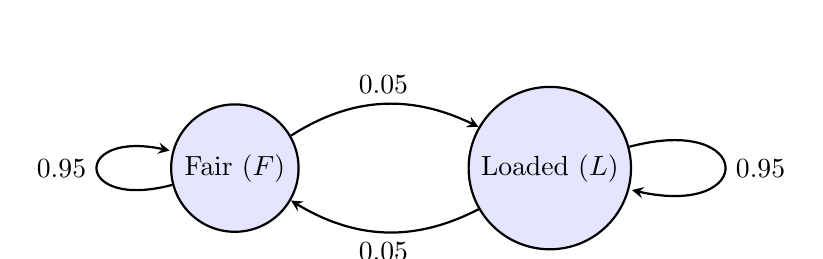
\begin{tikzpicture}[->, >=stealth, auto, node distance=4cm, thick, state/.style={circle, draw, minimum size=1.5cm, fill=blue!10}]
\node[state] (F) {Fair ($F$)};
\node[state] (L) [right of=F] {Loaded ($L$)};

\path
(F) edge [loop left] node {\(0.95\)} (F)
    edge [bend left] node {\(0.05\)} (L)
(L) edge [loop right] node {\(0.95\)} (L)
    edge [bend left] node {\(0.05\)} (F);
\end{tikzpicture}
\end{center}

We observe a sequence of die rolls (the emissions) but do not know which die the dealer is using (the hidden path). Our goal is to determine when the dealer is using the loaded die. 

\textbf{Example: The Dishonest Genome}\\
This maps directly to genomics. A genome might randomly transition between human DNA (Background) and integrated viral DNA. The observable alphabet is $\{A, C, G, T\}$. Viral DNA and Human DNA will have distinct emission probabilities for these nucleotides (e.g., varying GC-content), and transitions between them are rare but possible.

% [IMAGE: Header of the paper 'Prediction of Complete Gene Structures in Human Genomic DNA' by Burge and Karlin, introducing GENSCAN.]
\myimage{7_1/2.png}{Header of the paper 'Prediction of Complete Gene Structures in Human Genomic DNA' by Burge and Karlin, introducing GENSCAN.}
% [IMAGE: Complex HMM architecture (GENSCAN) for predicting protein-coding genes, showing hidden states for UTRs, Exons, Introns, and start/stop/splice signals across different reading frames.]

\section{The Six Algorithmic Settings for HMMs}

When working with HMMs, we address three main types of problems, each under two different constraints (evaluating a single specific path vs. evaluating all possible paths):

\begin{table}[h]
\centering
\begin{tabularx}{\textwidth}{l X X}
\toprule
\textbf{Task} & \textbf{One Path (Optimal)} & \textbf{All Paths (Summed)} \\
\midrule
\textbf{Evaluation} & 1. Scoring $x$ over the optimal path. & 2. Scoring $x$ over all paths (Forward algorithm). \\
\textbf{Decoding} & 3. Finding the best state sequence (Viterbi algorithm). & 4. Probabilistic label per position (Posterior decoding). \\
\textbf{Learning} & 5a. Supervised MLE (if labels known). \newline 5b. Viterbi training (if labels unknown). & 6. Baum-Welch / EM (if labels unknown). \\
\bottomrule
\end{tabularx}
\caption{The six algorithmic settings for handling HMMs in sequence analysis.}
\end{table}

\subsection{Evaluation: Scoring a Sequence}

\subsubsection{Setting 1: Scoring a Single Path (Joint Probability)}

If we are given an exact sequence of observations \( x \) and a specifically assumed hidden path \( \pi \), we calculate their joint probability by multiplying the transition probabilities along the path by the emission probabilities at each step:

\[ P(x, \pi) = P(x \mid \pi) P(\pi) = p(\pi_1) e_{\pi_1}(x_1) \prod_{i=1}^{N-1} a_{\pi_i \pi_{i+1}} e_{\pi_{i+1}}(x_{i+1}) \]

\textbf{Example:} Comparing paths in the Dishonest Casino.\\
Assume we observe the sequence \( x = 1, 2, 1, 5, 6, 2, 1, 6, 2, 4 \). Assuming an initial probability of 0.5 for starting in either state:
\begin{itemize}
    \item \textbf{All-Fair path (\(\pi = F, \dots, F\)):}
    \[ P(x, \text{all-Fair}) = 0.5 \times \left(\frac{1}{6}\right)^{10} \times (0.95)^9 \approx 5.2 \times 10^{-9} \]
    \item \textbf{All-Loaded path (\(\pi = L, \dots, L\)):}
    \[ P(x, \text{all-Loaded}) = 0.5 \times \left(\frac{1}{10}\right)^8 \times \left(\frac{1}{2}\right)^2 \times (0.95)^9 \approx 7.9 \times 10^{-10} \]
\end{itemize}
The all-Fair path is about 6.59 times more likely than the all-Loaded path for this particular sequence. 
\sta \textit{Note:} Joint probabilities approach zero rapidly, necessitating the use of log-scores to prevent computational underflow.

% INSERT /home/papagna/Projects/latex_bio/lex_md/07-Sequence_modeling-HMM_07-Sequence_modeling-HMM/imgs/cropped_page27_idx20.jpg

\subsubsection{Setting 2: Scoring All Paths (Forward Algorithm)}

To find the \textit{total} probability \( P(x) \) that the model generated the sequence, regardless of the specific path taken, we sum the joint probabilities over an exponential number of possible paths:
\[ P(x) = \sum_{\pi} P(x, \pi) \]

% INSERT /home/papagna/Projects/latex_bio/lex_md/07-Sequence_modeling-HMM_07-Sequence_modeling-HMM/imgs/cropped_page42_idx34.jpg

We compute this efficiently in $\mathcal{O}(K^2 N)$ time using dynamic programming via the \textbf{Forward Algorithm}. Let \( f_k(i) \) be the probability of generating the prefix sequence \( x_1 \dots x_i \) and ending in state \( k \).

\begin{itemize}
    \item \textbf{Initialization:} \( f_0(0) = 1 \), \( f_k(0) = 0 \) for all \( k > 0 \).
    \item \textbf{Iteration:} 
    \[ f_k(i) = e_k(x_i) \times \sum_j \left( a_{jk} f_j(i-1) \right) \]
    \item \textbf{Termination:} The total probability of the sequence is \( P(x) = \sum_k f_k(N) \).
\end{itemize}

% INSERT /home/papagna/Projects/latex_bio/insert/screenshot-2026-06-10_23-40-59.png

\subsection{Decoding: Finding the Hidden States}

\subsubsection{Setting 3: Decoding the Most Likely Path (Viterbi Algorithm)}

Given only the observed emissions \( x \), we usually want to find the single most likely sequence of hidden states \( \pi^* \) that generated it. The problem exhibits \textit{optimal substructure}: the best path reaching state $k$ at step $i$ is composed of the best path reaching some state $j$ at step $i-1$, followed by the optimal transition to $k$.

\begin{important}
  \textbf{Viterbi Algorithm:} A dynamic programming algorithm that computes the most likely sequence of hidden states. Let \( V_k(i) \) be the probability of the most likely path generating sequence $x_1 \dots x_i$ and ending in state $k$.
  \begin{itemize}
      \item \textbf{Initialization:} \( V_0(0) = 1 \); \( V_k(0) = 0 \) for all \( k > 0 \).
      \item \textbf{Iteration:} \( V_k(i) = e_k(x_i) \times \max_j (a_{jk} V_j(i-1)) \)
      \item \textbf{Termination:} \( P(x, \pi^*) = \max_k V_k(N) \)
  \end{itemize}
\end{important}

We keep pointers to the maximizing state \( j \) at each step to reconstruct the optimal path \(\pi^*\) via traceback. The time complexity is $\mathcal{O}(K^2N)$ and space complexity is $\mathcal{O}(KN)$.

\begin{minted}{python}
# [pseudocode]
def viterbi(obs, states, init_p, trans_p, emit_p):
    V = [{}] # DP matrix
    path = {}
    
    # Initialization
    for y in states:
        V[0][y] = init_p[y] * emit_p[y][obs[0]]
        path[y] = [y]
        
    # Iteration
    for t in range(1, len(obs)):
        V.append({})
        newpath = {}
        for y in states:
            (prob, state) = max((V[t-1][y0] * trans_p[y0][y] * emit_p[y][obs[t]], y0) 
                                for y0 in states)
            V[t][y] = prob
            newpath[y] = path[state] + [y]
        path = newpath
        
    # Termination
    (prob, state) = max((V[len(obs) - 1][y], y) for y in states)
    return prob, path[state]
\end{minted}

% INSERT /home/papagna/Projects/latex_bio/insert/screenshot-2026-06-10_23-36-23.png

% INSERT /home/papagna/Projects/latex_bio/insert/screenshot-2026-06-10_23-37-16.png

\textbf{Example: Viterbi Trace for a Viral (V) vs. Self (S) Genome Model} \\
Assume we observe the sequence \( x = (G, C, G, A, T) \).
Initial: \( p_V = 0.5, p_S = 0.5 \). \\
Transitions: \( a_{VV} = 0.15, a_{VS} = 0.85, a_{SV} = 0.05, a_{SS} = 0.95 \). \\
Emissions \( V \): \( G(0.33), C(0.33), A(0.17), T(0.17) \). \\
Emissions \( S \): \( G(0.25), C(0.25), A(0.25), T(0.25) \).

\begin{enumerate}
    \item \textbf{Initialization \( i=1 \) (Emission 'G'):}
    \( V_V(1) = 0.5 \times 0.33 = 0.165 \) \\
    \( V_S(1) = 0.5 \times 0.25 = 0.125 \)
    \item \textbf{Iteration \( i=2 \) (Emission 'C'):}
    \( V_V(2) = 0.33 \times \max(0.15 \times 0.165, 0.05 \times 0.125) \approx 8.17 \times 10^{-3} \) (from V). \\
    \( V_S(2) = 0.25 \times \max(0.85 \times 0.165, 0.95 \times 0.125) \approx 3.5 \times 10^{-2} \) (from V).
    \item \textbf{Termination \& Traceback:} Continuing to \( i=5 \), the highest probability ends in state \( S \). Tracing the max pointers backwards reveals the optimal path: \( V \to S \to S \to S \to S \). 
\end{enumerate}
This demonstrates how the high transition probability from Viral to Self (\(0.85\)) dominates, making it optimal to start in the viral state but immediately switch to the self state.

% INSERT /home/papagna/Projects/latex_bio/insert/screenshot-2026-06-10_23-38-12.png

\subsubsection{Setting 4: Decoding All Paths (Posterior Decoding)}

Viterbi gives the single best path, but it ignores the probability mass of all other valid paths. To find the most likely state for a \textit{specific position} \( i \) averaged over all paths, we use \textbf{Posterior Decoding}.

% INSERT /home/papagna/Projects/latex_bio/lex_md/07-Sequence_modeling-HMM_07-Sequence_modeling-HMM/imgs/cropped_page64_idx60.jpg

We combine the \textbf{Forward algorithm} (how we got to position \( i \)) and the \textbf{Backward algorithm} (the probability of observing the remainder of the sequence given we are at state \( k \) at position \( i \)).

\textbf{The Backward Algorithm:}
Define \( b_k(i) = P(x_{i+1} \dots x_N \mid \pi_i = k) \).
\begin{itemize}
    \item \textbf{Initialization:} \( b_k(N) = a_{k0} \) (or 1 if end state transitions are uniform) for all \( k \).
    \item \textbf{Iteration:} (Working backwards from \( N-1 \) down to 1):
    \[ b_k(i) = \sum_l \left( e_l(x_{i+1}) \cdot a_{kl} \cdot b_l(i+1) \right) \]
\end{itemize}

% INSERT /home/papagna/Projects/latex_bio/insert/screenshot-2026-06-10_23-45-13.png

By multiplying the forward and backward probabilities, we isolate the probability of being in state \( k \) at position \( i \) given the entire sequence \( x \):
\[ P(\pi_i = k \mid x) = \frac{f_k(i) \cdot b_k(i)}{P(x)} \]
where \( P(x) \) can be found via the Forward algorithm, or computed as \( P(x) = \sum_l a_{0l} e_l(x_1) b_l(1) \).

\sta Posterior decoding provides the highest-confidence state at each independent position. However, because it optimizes locally, the resulting sequence of states might contain structurally impossible transitions (e.g., jumping from a Promoter directly to an Intron).

\subsection{Learning: Training HMM Parameters}

Before an HMM can decode a genome, we must estimate its parameters: transition probabilities (\( a_{kl} \)) and emission probabilities (\( e_k(x) \)).

% INSERT /home/papagna/Projects/latex_bio/insert/screenshot-2026-06-10_23-49-03.png

\subsubsection{Setting 5a: Supervised Learning (Known Labels - When the right answer is known)}

When we have training data fully annotated with true hidden states, learning uses Maximum Likelihood Estimation (MLE) by simply counting frequencies:
\[ a_{kl} = \frac{A_{kl}}{\sum_i A_{ki}} \quad \text{and} \quad e_k(b) = \frac{E_k(b)}{\sum_c E_k(c)} \]

% INSERT /home/papagna/Projects/latex_bio/insert/screenshot-2026-06-10_23-51-31.png

\sta \textbf{Pseudocounts:} Given limited data, unobserved events might get a strict probability of 0, which is fatal in HMMs (multiplying by 0 negates an entire path). We resolve this by adding artificial constants, or \textbf{pseudocounts} (\( r_{kl}, r_k(b) \)), to all observed counts before normalization:
\[ A_{kl} = (\text{observed count}) + r_{kl} \]
Larger pseudocounts reflect strong prior beliefs, while small pseudocounts (\( \epsilon \ll 1 \)) act merely as regularizers to prevent zeroes.

\subsubsection{Setting 6: Unsupervised Learning (Unknown Labels - When the right answer is unknown)}

When we have raw unlabelled sequence data, we bootstrap parameters iteratively.

\textbf{Viterbi Training (Hard Assignments):}
1. Guess initial parameters.
2. Run Viterbi decoding to generate the single most likely hidden path.
3. Treat this generated path as labeled data, and update parameters using supervised MLE.
4. Iterate until convergence.
\textit{Note:} This is fast but suboptimal because it places 100\% of the statistical weight on the single Viterbi path.

\textbf{Expectation Maximization / The Baum-Welch Algorithm (Soft Assignments):}
To properly account for all possible paths, we use the Baum-Welch algorithm, an application of Expectation Maximization (EM).

\begin{important}
  \textbf{Baum-Welch Algorithm:} An unsupervised EM algorithm that iteratively refines HMM parameters by utilizing the Forward and Backward probabilities to weigh the contributions of all possible hidden paths.
\end{important}

\begin{enumerate}
    \item \textbf{Initialization:} Start with estimated model parameters.
    \item \textbf{E-Step (Expectation):} Run the Forward and Backward algorithms. For every position \( i \), compute the expected probability that a specific transition \( k \to l \) occurred, based on the posterior distribution:
    \[ P(\pi_i = k, \pi_{i+1} = l \mid x, \theta) = \frac{f_k(i) \cdot a_{kl} \cdot e_l(x_{i+1}) \cdot b_l(i+1)}{P(x \mid \theta)} \]
    \item \textbf{M-Step (Maximization):} Sum these expected probabilities over the entire sequence to get the new expected transition counts \( A_{kl} \) and expected emission counts \( E_k(b) \). Recalculate \( a_{kl} \) and \( e_k(b) \) by normalizing these sums to maximize the log-likelihood.
    \item \textbf{Iteration:} Repeat E and M steps. The total likelihood \( P(x \mid \theta) \) is mathematically guaranteed to increase with each iteration. Stop when it converges.
\end{enumerate}

\sta Baum-Welch is guaranteed to find a local maximum, but not necessarily the global optimum. Running the algorithm multiple times from different random initializations helps explore the parameter space.

\section{Enhancing the State Space to Include Memory}

By mathematical definition, Markov models are memoryless. The current state determines the probabilities independent of the prior path. However, biology often requires memory. For example, in CpG islands, seeing a \( C \) significantly increases the probability that the next nucleotide is a \( G \).

\textbf{Solution: Expand the state space.}
We embed historical context into the identity of the current state itself. For a CpG island detector, instead of 2 states (CpG-rich vs. Background), we create 8 states:
\begin{itemize}
    \item \textbf{CpG-rich states (\(+\)):} \( A_+, C_+, G_+, T_+ \) (observed inside an island)
    \item \textbf{Background states (\(-\)):} \( A_-, C_-, G_-, T_- \) (observed outside an island)
\end{itemize}

% [IMAGE: Graph showing 8 nodes instead of 2. The four '+' nodes represent nucleotides emitted inside a CpG island, and the four '-' nodes represent nucleotides emitted in background DNA. Transition arrows between C+ and G+ are given very high weight to simulate the biological prevalence of CpG dinucleotides.]
\myimage{7_1/4.png}{Graph showing 8 nodes instead of 2. The four '+' nodes represent nucleotides emitted inside a CpG island, and the four '-' nodes represent nucleotides emitted in background DNA. Transition arrows between C+ and G+ are given very high weight to simulate the biological prevalence of CpG dinucleotides.}

If the system emits a `C` while in a CpG-island, it enters the \( C_+ \) state. From \( C_+ \), we assign a highly inflated transition probability \( a_{C_+ \to G_+} \), accurately simulating the di-nucleotide frequency while strictly adhering to the memoryless rules.

Similarly, in protein-coding gene models (like GENSCAN), expanding state space allows us to track reading frames (codons) across spliced introns by explicitly defining states like \( E_0, E_1, E_2 \) for exons and \( I_0, I_1, I_2 \) for introns depending on the reading frame offset.


\end{document}
